% Options for packages loaded elsewhere
\PassOptionsToPackage{unicode}{hyperref}
\PassOptionsToPackage{hyphens}{url}
\documentclass[
  french,
]{article}
\usepackage{xcolor}
\usepackage[margin=1in]{geometry}
\usepackage{amsmath,amssymb}
\setcounter{secnumdepth}{5}
\usepackage{iftex}
\ifPDFTeX
  \usepackage[T1]{fontenc}
  \usepackage[utf8]{inputenc}
  \usepackage{textcomp} % provide euro and other symbols
\else % if luatex or xetex
  \usepackage{unicode-math} % this also loads fontspec
  \defaultfontfeatures{Scale=MatchLowercase}
  \defaultfontfeatures[\rmfamily]{Ligatures=TeX,Scale=1}
\fi
\usepackage{lmodern}
\ifPDFTeX\else
  % xetex/luatex font selection
\fi
% Use upquote if available, for straight quotes in verbatim environments
\IfFileExists{upquote.sty}{\usepackage{upquote}}{}
\IfFileExists{microtype.sty}{% use microtype if available
  \usepackage[]{microtype}
  \UseMicrotypeSet[protrusion]{basicmath} % disable protrusion for tt fonts
}{}
\makeatletter
\@ifundefined{KOMAClassName}{% if non-KOMA class
  \IfFileExists{parskip.sty}{%
    \usepackage{parskip}
  }{% else
    \setlength{\parindent}{0pt}
    \setlength{\parskip}{6pt plus 2pt minus 1pt}}
}{% if KOMA class
  \KOMAoptions{parskip=half}}
\makeatother
\usepackage{color}
\usepackage{fancyvrb}
\newcommand{\VerbBar}{|}
\newcommand{\VERB}{\Verb[commandchars=\\\{\}]}
\DefineVerbatimEnvironment{Highlighting}{Verbatim}{commandchars=\\\{\}}
% Add ',fontsize=\small' for more characters per line
\usepackage{framed}
\definecolor{shadecolor}{RGB}{248,248,248}
\newenvironment{Shaded}{\begin{snugshade}}{\end{snugshade}}
\newcommand{\AlertTok}[1]{\textcolor[rgb]{0.94,0.16,0.16}{#1}}
\newcommand{\AnnotationTok}[1]{\textcolor[rgb]{0.56,0.35,0.01}{\textbf{\textit{#1}}}}
\newcommand{\AttributeTok}[1]{\textcolor[rgb]{0.13,0.29,0.53}{#1}}
\newcommand{\BaseNTok}[1]{\textcolor[rgb]{0.00,0.00,0.81}{#1}}
\newcommand{\BuiltInTok}[1]{#1}
\newcommand{\CharTok}[1]{\textcolor[rgb]{0.31,0.60,0.02}{#1}}
\newcommand{\CommentTok}[1]{\textcolor[rgb]{0.56,0.35,0.01}{\textit{#1}}}
\newcommand{\CommentVarTok}[1]{\textcolor[rgb]{0.56,0.35,0.01}{\textbf{\textit{#1}}}}
\newcommand{\ConstantTok}[1]{\textcolor[rgb]{0.56,0.35,0.01}{#1}}
\newcommand{\ControlFlowTok}[1]{\textcolor[rgb]{0.13,0.29,0.53}{\textbf{#1}}}
\newcommand{\DataTypeTok}[1]{\textcolor[rgb]{0.13,0.29,0.53}{#1}}
\newcommand{\DecValTok}[1]{\textcolor[rgb]{0.00,0.00,0.81}{#1}}
\newcommand{\DocumentationTok}[1]{\textcolor[rgb]{0.56,0.35,0.01}{\textbf{\textit{#1}}}}
\newcommand{\ErrorTok}[1]{\textcolor[rgb]{0.64,0.00,0.00}{\textbf{#1}}}
\newcommand{\ExtensionTok}[1]{#1}
\newcommand{\FloatTok}[1]{\textcolor[rgb]{0.00,0.00,0.81}{#1}}
\newcommand{\FunctionTok}[1]{\textcolor[rgb]{0.13,0.29,0.53}{\textbf{#1}}}
\newcommand{\ImportTok}[1]{#1}
\newcommand{\InformationTok}[1]{\textcolor[rgb]{0.56,0.35,0.01}{\textbf{\textit{#1}}}}
\newcommand{\KeywordTok}[1]{\textcolor[rgb]{0.13,0.29,0.53}{\textbf{#1}}}
\newcommand{\NormalTok}[1]{#1}
\newcommand{\OperatorTok}[1]{\textcolor[rgb]{0.81,0.36,0.00}{\textbf{#1}}}
\newcommand{\OtherTok}[1]{\textcolor[rgb]{0.56,0.35,0.01}{#1}}
\newcommand{\PreprocessorTok}[1]{\textcolor[rgb]{0.56,0.35,0.01}{\textit{#1}}}
\newcommand{\RegionMarkerTok}[1]{#1}
\newcommand{\SpecialCharTok}[1]{\textcolor[rgb]{0.81,0.36,0.00}{\textbf{#1}}}
\newcommand{\SpecialStringTok}[1]{\textcolor[rgb]{0.31,0.60,0.02}{#1}}
\newcommand{\StringTok}[1]{\textcolor[rgb]{0.31,0.60,0.02}{#1}}
\newcommand{\VariableTok}[1]{\textcolor[rgb]{0.00,0.00,0.00}{#1}}
\newcommand{\VerbatimStringTok}[1]{\textcolor[rgb]{0.31,0.60,0.02}{#1}}
\newcommand{\WarningTok}[1]{\textcolor[rgb]{0.56,0.35,0.01}{\textbf{\textit{#1}}}}
\usepackage{longtable,booktabs,array}
\usepackage{calc} % for calculating minipage widths
% Correct order of tables after \paragraph or \subparagraph
\usepackage{etoolbox}
\makeatletter
\patchcmd\longtable{\par}{\if@noskipsec\mbox{}\fi\par}{}{}
\makeatother
% Allow footnotes in longtable head/foot
\IfFileExists{footnotehyper.sty}{\usepackage{footnotehyper}}{\usepackage{footnote}}
\makesavenoteenv{longtable}
\usepackage{graphicx}
\makeatletter
\newsavebox\pandoc@box
\newcommand*\pandocbounded[1]{% scales image to fit in text height/width
  \sbox\pandoc@box{#1}%
  \Gscale@div\@tempa{\textheight}{\dimexpr\ht\pandoc@box+\dp\pandoc@box\relax}%
  \Gscale@div\@tempb{\linewidth}{\wd\pandoc@box}%
  \ifdim\@tempb\p@<\@tempa\p@\let\@tempa\@tempb\fi% select the smaller of both
  \ifdim\@tempa\p@<\p@\scalebox{\@tempa}{\usebox\pandoc@box}%
  \else\usebox{\pandoc@box}%
  \fi%
}
% Set default figure placement to htbp
\def\fps@figure{htbp}
\makeatother
\ifLuaTeX
\usepackage[bidi=basic]{babel}
\else
\usepackage[bidi=default]{babel}
\fi
% get rid of language-specific shorthands (see #6817):
\let\LanguageShortHands\languageshorthands
\def\languageshorthands#1{}
\setlength{\emergencystretch}{3em} % prevent overfull lines
\providecommand{\tightlist}{%
  \setlength{\itemsep}{0pt}\setlength{\parskip}{0pt}}
\usepackage{bookmark}
\IfFileExists{xurl.sty}{\usepackage{xurl}}{} % add URL line breaks if available
\urlstyle{same}
\hypersetup{
  pdftitle={Telco's intern},
  pdfauthor={Bastien Baranoff},
  pdflang={fr},
  hidelinks,
  pdfcreator={LaTeX via pandoc}}

\title{Telco's intern}
\author{Bastien Baranoff}
\date{2026-03-06}

\begin{document}
\maketitle

{
\setcounter{tocdepth}{2}
\tableofcontents
}
\pandocbounded{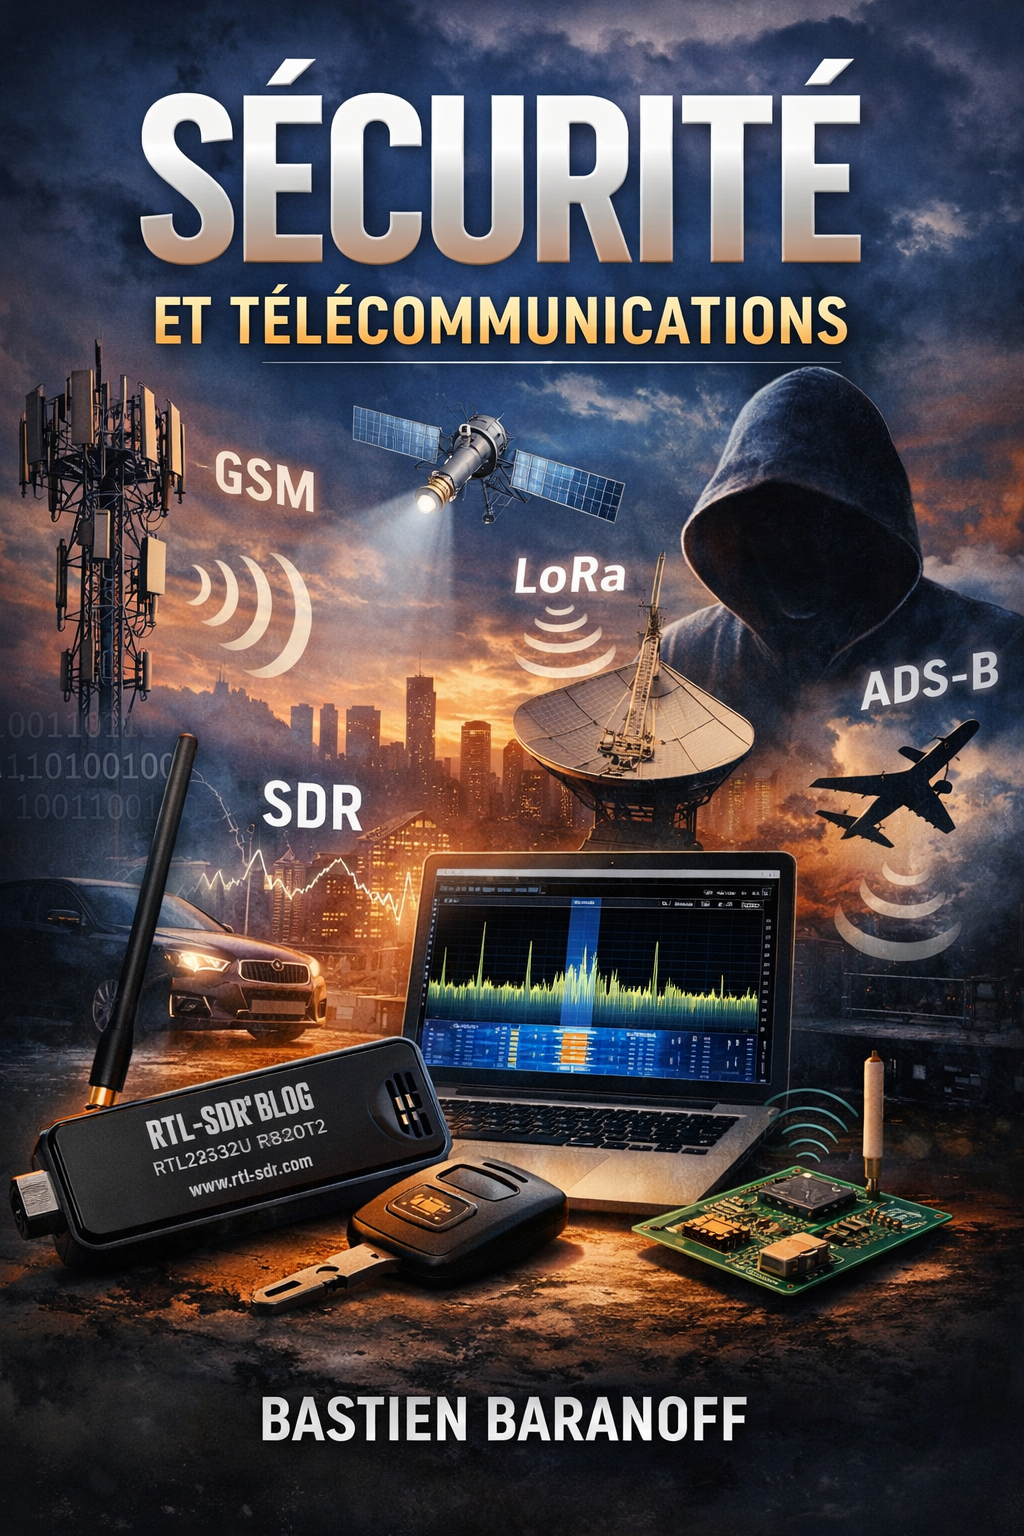
\includegraphics[keepaspectratio]{pictures/couverture.png}}

\section{Un livre sur mon expérience en
radio-télécommunications}\label{un-livre-sur-mon-expuxe9rience-en-radio-tuxe9luxe9communications}

J'espère que vous apprécierez.

\section{INTRODUCTION}\label{introduction}

\subsection{Transmettre l'information plus vite que
l'homme}\label{transmettre-linformation-plus-vite-que-lhomme}

Avant l'électricité, la communication à distance était limitée par une
contrainte simple : \textbf{la vitesse d'un messager}.

Pendant des millénaires, transmettre une information signifiait déplacer
physiquement un objet ou une personne :

\begin{itemize}
\tightlist
\item
  un cavalier
\item
  un navire
\item
  un pigeon voyageur
\item
  un courrier postal
\end{itemize}

La vitesse maximale d'une information était donc celle du transport.

Un message envoyé de Paris à Londres pouvait prendre \textbf{plusieurs
jours}.\\
Une information stratégique --- militaire, politique ou économique ---
arrivait souvent \textbf{trop tard pour être utile}.

Certaines civilisations ont tenté de contourner cette limite.

Par exemple :

\begin{itemize}
\tightlist
\item
  \textbf{signaux de fumée}
\item
  \textbf{feux de signalisation}
\item
  \textbf{sémaphores optiques}
\item
  \textbf{télégraphes optiques}
\end{itemize}

Le système de \textbf{Claude Chappe}, développé en France à la fin du
XVIII siècle, est l'un des premiers véritables réseaux de communication
à distance.\\
Il utilisait des \textbf{tours équipées de bras mobiles} visibles à
plusieurs kilomètres.

Chaque position des bras représentait un symbole.

Le message se propageait de tour en tour :

\begin{verbatim}

Tour A → Tour B → Tour C → Tour D
\end{verbatim}

Ce système permettait déjà une transmission beaucoup plus rapide qu'un
cavalier.

Cependant il avait plusieurs limites importantes :

\begin{itemize}
\tightlist
\item
  dépendance à la \textbf{visibilité}
\item
  impossibilité de fonctionner \textbf{la nuit}
\item
  sensibilité aux \textbf{conditions météorologiques}
\item
  infrastructure lourde à maintenir
\end{itemize}

Malgré ces contraintes, le télégraphe optique a introduit une idée
fondamentale :

\textbf{l'information peut être codée en symboles et transmise à
distance indépendamment du support physique du message.}

Cette idée ouvre la porte à une révolution.

Car une question devient alors possible :

\begin{quote}
et si l'information pouvait voyager non plus à la vitesse d'un
cheval\ldots{}\\
mais à la vitesse de l'électricité ?
\end{quote}

\subsection{L'électricité devient un
langage}\label{luxe9lectricituxe9-devient-un-langage}

Au début du XIX siècle, les progrès en \textbf{électricité et en
électromagnétisme} transforment progressivement la manière dont les
scientifiques comprennent les phénomènes physiques.

Les expériences menées par \textbf{Ørsted}, \textbf{Ampère} et
\textbf{Faraday} montrent qu'il existe un lien profond entre
\textbf{électricité et magnétisme}.\\
Un courant électrique peut produire un champ magnétique, et inversement
un champ magnétique variable peut produire un courant.

Cette relation ouvre une possibilité nouvelle : utiliser l'électricité
pour \textbf{transmettre un signal à distance dans un fil conducteur}.

Le principe est simple.

Un circuit électrique peut être \textbf{ouvert ou fermé}.\\
Cette variation peut être détectée à l'autre extrémité du fil.

Autrement dit, un signal électrique peut transporter \textbf{de
l'information}.

Dans les années 1830--1840, plusieurs inventeurs expérimentent ce
principe.\\
Le système qui va s'imposer est celui de \textbf{Samuel Morse}.

Son idée est élégante :

\begin{itemize}
\tightlist
\item
  l'électricité sert uniquement à transmettre un \textbf{signal simple}
\item
  le message est codé sous forme de \textbf{symboles courts et longs}
\end{itemize}

Ce système devient le \textbf{code Morse}.

Par exemple :

\begin{verbatim}

A  .-
B  -...
C  -.-.
\end{verbatim}

Chaque lettre correspond à une combinaison de :

\begin{itemize}
\tightlist
\item
  \textbf{points}
\item
  \textbf{traits}
\end{itemize}

Le signal électrique envoyé dans le fil actionne un
\textbf{électroaimant} à l'autre extrémité, qui produit un clic
mécanique.

L'opérateur entend donc une séquence de sons qu'il peut traduire en
lettres.

Un message devient ainsi une \textbf{suite de signaux électriques}.

Le télégraphe électrique marque une rupture majeure dans l'histoire des
communications :

\begin{itemize}
\tightlist
\item
  la transmission n'est plus limitée par la vitesse du transport
  physique
\item
  l'information peut voyager \textbf{quasi instantanément} sur de
  longues distances
\end{itemize}

Les réseaux télégraphiques se déploient rapidement le long des
\textbf{voies ferrées} et entre les grandes villes.

En 1858, un événement spectaculaire illustre la puissance de cette
technologie :

le premier \textbf{câble télégraphique transatlantique} est posé entre
l'Europe et l'Amérique.

Pour la première fois dans l'histoire humaine, un message peut traverser
l'océan en \textbf{quelques minutes}.

Le monde vient d'entrer dans l'ère des \textbf{réseaux de
communication}.

\subsection{La voix dans un fil : le
téléphone}\label{la-voix-dans-un-fil-le-tuxe9luxe9phone}

Le télégraphe a permis de transmettre des \textbf{symboles} à
distance.\\
Mais une question restait ouverte :

\begin{quote}
peut-on transmettre \textbf{directement la voix humaine} ?
\end{quote}

La voix est un phénomène physique :\\
ce sont \textbf{des vibrations de l'air} produites par les cordes
vocales.

Ces vibrations ont deux caractéristiques principales :

\begin{itemize}
\tightlist
\item
  \textbf{fréquence}
\item
  \textbf{amplitude}
\end{itemize}

Autrement dit, la voix est déjà un \textbf{signal analogique}.

L'idée du téléphone est donc de transformer ces vibrations en
\textbf{signal électrique équivalent}, de le transmettre dans un fil,
puis de le reconvertir en \textbf{vibration sonore}.

Le principe du premier téléphone est étonnamment simple.

\begin{verbatim}

voix → membrane → variation électrique → fil → membrane → son
\end{verbatim}

Le dispositif comprend trois éléments essentiels :

\begin{itemize}
\tightlist
\item
  une \textbf{membrane} qui vibre avec la voix
\item
  un \textbf{transducteur électromagnétique}
\item
  un \textbf{fil conducteur}
\end{itemize}

Lorsque quelqu'un parle :

\begin{enumerate}
\def\labelenumi{\arabic{enumi}.}
\tightlist
\item
  la membrane vibre\\
\item
  ces vibrations modifient un champ magnétique\\
\item
  cela crée un \textbf{courant électrique variable} dans le fil\\
\item
  ce courant est reproduit à l'autre extrémité\\
\item
  une seconde membrane recrée les vibrations sonores
\end{enumerate}

La parole devient donc une \textbf{onde électrique analogique}.

Ce principe est démontré en 1876 par \textbf{Alexander Graham Bell}, qui
dépose l'un des brevets fondateurs du téléphone.

Sa première phrase célèbre aurait été :

\begin{quote}
\emph{``Mr.~Watson, come here, I want to see you.''}
\end{quote}

Cependant, l'histoire du téléphone est plus complexe qu'un seul
inventeur.

Plusieurs chercheurs travaillaient simultanément sur des idées
similaires :

\begin{itemize}
\tightlist
\item
  \textbf{Antonio Meucci}
\item
  \textbf{Elisha Gray}
\item
  \textbf{Johann Philipp Reis}
\end{itemize}

Elisha Gray aurait même déposé une description technique \textbf{le même
jour que Bell}, à quelques heures près.

Le téléphone n'est donc pas seulement une invention isolée.\\
C'est le résultat d'une \textbf{convergence technologique} rendue
possible par les progrès de l'électricité et du télégraphe.

Mais une conséquence va changer le monde.

Avec le téléphone, la communication ne passe plus par un opérateur qui
décode des symboles.

Elle devient \textbf{instantanée et naturelle}.

La voix humaine peut désormais voyager à travers un réseau électrique.

Et pour faire fonctionner ce réseau, il faut inventer de nouvelles
infrastructures :

\begin{itemize}
\tightlist
\item
  \textbf{centraux téléphoniques}
\item
  \textbf{commutation}
\item
  \textbf{numérotation}
\item
  \textbf{gestion des abonnés}
\end{itemize}

Ces concepts deviendront la base de toute l'architecture des
\textbf{télécommunications modernes}.

\subsection{L'unification de l'électricité et du magnétisme :
Maxwell}\label{lunification-de-luxe9lectricituxe9-et-du-magnuxe9tisme-maxwell}

Pendant que le téléphone et le télégraphe se développent, la physique
poursuit une question plus fondamentale :

\textbf{quelle est la nature de l'électricité et du magnétisme ?}

Au milieu du XIX siècle, les expériences de \textbf{Faraday} avaient
déjà montré qu'un champ magnétique variable pouvait produire un courant
électrique.\\
Mais il manquait encore une \textbf{théorie unifiée} capable de décrire
ces phénomènes.

C'est le physicien écossais \textbf{James Clerk Maxwell} qui va apporter
cette réponse.

En 1864, Maxwell publie une série d'équations qui décrivent complètement
le comportement des \textbf{champs électriques et magnétiques}.\\
Ces équations montrent que l'électricité et le magnétisme ne sont pas
deux phénomènes séparés, mais \textbf{deux aspects d'un même champ
électromagnétique}.

Sous leur forme moderne, les équations de Maxwell s'écrivent :

\[
\nabla \cdot \mathbf{E} = \frac{\rho}{\varepsilon_0}
\]

Cette équation indique que les \textbf{charges électriques} sont la
source des champs électriques.

\[
\nabla \cdot \mathbf{B} = 0
\]

Elle exprime qu'il n'existe pas de \textbf{monopôle magnétique} : les
lignes de champ magnétique forment toujours des boucles fermées.

\[
\nabla \times \mathbf{E} = -\frac{\partial \mathbf{B}}{\partial t}
\]

Une variation d'un \textbf{champ magnétique} crée un \textbf{champ
électrique}.

\[
\nabla \times \mathbf{B} =
\mu_0 \mathbf{J} + \mu_0 \varepsilon_0
\frac{\partial \mathbf{E}}{\partial t}
\]

Un courant électrique ou une variation du champ électrique produit un
\textbf{champ magnétique}.

Ces équations contiennent une conséquence remarquable.

Si un champ électrique varie dans le temps, il crée un champ
magnétique.\\
Ce champ magnétique variable recrée à son tour un champ électrique.

Le résultat est une \textbf{onde électromagnétique auto-propagée}.

Maxwell calcule alors la vitesse de propagation de cette onde :

\[
c = \frac{1}{\sqrt{\mu_0 \varepsilon_0}}
\]

Cette vitesse correspond exactement à la \textbf{vitesse de la lumière}.

La conclusion est spectaculaire :

\begin{quote}
\textbf{la lumière est une onde électromagnétique.}
\end{quote}

Et si la lumière est une onde électromagnétique, alors d'autres ondes
similaires doivent exister.

Des ondes qui pourraient transporter de l'énergie\ldots{}\\
ou même \textbf{de l'information}.

Cette prédiction théorique ouvrira la voie à une nouvelle révolution :

la \textbf{communication sans fil}.

\subsection{La preuve expérimentale :
Hertz}\label{la-preuve-expuxe9rimentale-hertz}

Une théorie physique ne devient réellement solide que lorsqu'elle est
\textbf{vérifiée expérimentalement}.\\
Les équations de Maxwell prédisaient l'existence d'ondes
électromagnétiques, mais encore fallait-il démontrer qu'elles pouvaient
être \textbf{produites et détectées}.

C'est le physicien allemand \textbf{Heinrich Hertz} qui réalisera cette
démonstration en 1887.

Hertz conçoit une expérience simple mais ingénieuse.\\
Il utilise un \textbf{oscillateur électrique} composé de deux électrodes
séparées par un petit espace.\\
Lorsqu'une haute tension est appliquée, une \textbf{étincelle} apparaît
entre les électrodes.

Cette décharge produit un courant oscillant très rapide, qui génère un
\textbf{champ électromagnétique variable}.

Autrement dit, une \textbf{onde électromagnétique} est émise dans
l'espace.

Pour détecter cette onde, Hertz utilise un dispositif tout aussi simple
:

\begin{verbatim}

antenne → boucle métallique → petite étincelle
\end{verbatim}

Lorsque l'onde électromagnétique atteint la boucle métallique, un
courant est induit et une \textbf{minuscule étincelle} apparaît dans
l'interrupteur de la boucle.

Cela prouve que l'énergie a voyagé \textbf{dans l'air, sans fil}.

Hertz réalise plusieurs expériences pour vérifier les propriétés de ces
ondes :

\begin{itemize}
\tightlist
\item
  \textbf{réflexion}
\item
  \textbf{réfraction}
\item
  \textbf{interférences}
\item
  \textbf{polarisation}
\end{itemize}

Les ondes qu'il observe se comportent exactement comme la
\textbf{lumière}.

La prédiction de Maxwell est donc confirmée.

Cependant, Hertz lui-même ne voit pas d'application pratique à sa
découverte.\\
Lorsqu'on lui demande à quoi peuvent servir ces ondes, il répond
simplement :

\begin{quote}
« Je suppose que cela n'a aucune utilité\ldots{} c'est juste une
expérience qui prouve que Maxwell avait raison. »
\end{quote}

Comme souvent dans l'histoire des sciences, une découverte fondamentale
attendra qu'un autre esprit en imagine l'usage.

Quelques années plus tard, un ingénieur italien comprendra que ces ondes
peuvent être utilisées pour \textbf{transmettre des messages à
distance}.

Cet ingénieur s'appelle \textbf{Guglielmo Marconi}.

\subsection{De la radio à la communication
mobile}\label{de-la-radio-uxe0-la-communication-mobile}

La radio de Marconi permettait déjà de transmettre de l'information sans
fil.\\
Mais ces systèmes restaient principalement \textbf{point à point} :

\begin{itemize}
\tightlist
\item
  navire ↔ station côtière\\
\item
  station ↔ station\\
\item
  émetteur ↔ récepteur
\end{itemize}

Ils ne formaient pas encore un \textbf{réseau structuré} capable de
gérer des millions d'utilisateurs.

Pendant la première moitié du XX siècle, la radio évolue rapidement.\\
Les ingénieurs développent de nouvelles techniques pour transporter plus
d'information et améliorer la qualité du signal.

Par exemple :

\begin{itemize}
\tightlist
\item
  \textbf{modulation d'amplitude (AM)}\\
\item
  \textbf{modulation de fréquence (FM)}\\
\item
  \textbf{multiplexage fréquentiel}
\end{itemize}

Ces techniques permettent de transporter :

\begin{itemize}
\tightlist
\item
  de la \textbf{voix}
\item
  de la \textbf{musique}
\item
  des \textbf{signaux de contrôle}
\end{itemize}

La radio devient alors un véritable \textbf{média de communication de
masse}.

Cependant, un problème technique apparaît rapidement.

Le spectre radio est une \textbf{ressource limitée}.

Deux émetteurs utilisant la même fréquence dans la même zone produisent
des \textbf{interférences}.

Pour résoudre ce problème, les ingénieurs introduisent un concept
fondamental :\\
la \textbf{cellularisation du réseau}.

L'idée consiste à diviser le territoire en \textbf{cellules radio}.

\begin{verbatim}

cellule A | cellule B | cellule C
\end{verbatim}

Chaque cellule utilise un ensemble de fréquences spécifique.

Lorsqu'un utilisateur se déplace :

\begin{itemize}
\tightlist
\item
  le réseau détecte sa position
\item
  la communication est transférée vers une \textbf{nouvelle cellule}
\end{itemize}

Ce mécanisme s'appelle le \textbf{handover}.

Cette architecture transforme complètement la communication radio.

On ne parle plus simplement d'un émetteur et d'un récepteur, mais d'un
\textbf{réseau distribué d'antennes} capable de :

\begin{itemize}
\tightlist
\item
  gérer la mobilité
\item
  partager le spectre radio
\item
  connecter simultanément des millions d'utilisateurs
\end{itemize}

C'est la naissance du \textbf{réseau cellulaire}.

Dans les années 1980, cette architecture devient la base des premiers
réseaux mobiles numériques.

Le standard qui va s'imposer en Europe et dans une grande partie du
monde s'appelle :

\textbf{GSM --- Global System for Mobile Communications.}

Les réseaux cellulaires modernes reposent alors sur trois éléments
essentiels :

\begin{itemize}
\tightlist
\item
  un \textbf{terminal mobile} (le téléphone)
\item
  une \textbf{station de base radio}
\item
  un \textbf{réseau cœur} qui gère les abonnés et les appels
\end{itemize}

Cette architecture constitue le fondement des systèmes mobiles modernes
:

\begin{itemize}
\tightlist
\item
  GSM (2G)
\item
  UMTS (3G)
\item
  LTE (4G)
\item
  5G
\end{itemize}

Cependant, pendant longtemps, ces réseaux sont restés \textbf{fermés et
difficiles à étudier}.

Les équipements radio nécessaires étaient extrêmement coûteux et
réservés aux opérateurs ou aux laboratoires industriels.

Cette situation va changer radicalement avec l'apparition d'une nouvelle
technologie :

les \textbf{Software Defined Radios}.

\subsection{Les Software Defined
Radios}\label{les-software-defined-radios}

Pendant longtemps, étudier un réseau radio nécessitait des équipements
spécialisés extrêmement coûteux.\\
Les analyseurs RF, les stations de base expérimentales ou les
simulateurs de protocole étaient généralement réservés :

\begin{itemize}
\tightlist
\item
  aux opérateurs télécom
\item
  aux fabricants d'équipements
\item
  aux laboratoires de recherche
\end{itemize}

Pour un ingénieur indépendant ou un étudiant, accéder à ces outils était
pratiquement impossible.

La situation change profondément au début des années 2000 avec
l'apparition des \textbf{Software Defined Radios (SDR)}.

Le principe est simple : déplacer la majorité des fonctions radio
\textbf{du matériel vers le logiciel}.

Dans une radio traditionnelle, la chaîne de traitement est composée de
circuits analogiques spécialisés :

\begin{verbatim}

antenne → filtre RF → mélangeur → démodulateur → données
\end{verbatim}

Chaque fonction est réalisée par un composant électronique dédié.\\
Le comportement du système est donc \textbf{figé par le matériel}.

Avec un SDR, l'architecture est différente.

\begin{verbatim}

antenne → convertisseur ADC/DAC → traitement logiciel
\end{verbatim}

Le signal radio est numérisé très tôt, puis toutes les opérations sont
réalisées par logiciel :

\begin{itemize}
\tightlist
\item
  filtrage
\item
  modulation
\item
  démodulation
\item
  décodage de protocole
\end{itemize}

Cela transforme la radio en \textbf{système programmable}.

Le même matériel peut être utilisé pour :

\begin{itemize}
\tightlist
\item
  écouter la radio FM
\item
  analyser un signal GSM
\item
  décoder des trames ADS-B
\item
  expérimenter avec LoRa
\item
  étudier les réseaux LTE
\end{itemize}

Autrement dit, la radio devient une \textbf{plateforme de recherche et
d'expérimentation}.

L'apparition de matériels relativement accessibles, comme :

\begin{itemize}
\tightlist
\item
  \textbf{RTL-SDR}
\item
  \textbf{USRP}
\item
  \textbf{HackRF}
\item
  \textbf{LimeSDR}
\end{itemize}

a ouvert l'étude des systèmes radio à une communauté beaucoup plus
large.

Associés à des outils logiciels comme :

\begin{itemize}
\tightlist
\item
  \textbf{GNU Radio}
\item
  \textbf{gr-gsm}
\item
  \textbf{srsRAN}
\item
  \textbf{Osmocom}
\end{itemize}

ces dispositifs permettent aujourd'hui de reconstruire des systèmes
radio complexes avec un simple ordinateur.

Les réseaux cellulaires, longtemps considérés comme des infrastructures
opaques et inaccessibles, deviennent ainsi \textbf{des systèmes
observables et reproductibles}.

C'est précisément cette évolution qui rend possible le type
d'expérimentation présenté dans ce livre.

\section{Objectif du livre}\label{objectif-du-livre}

Les télécommunications modernes reposent sur une infrastructure
extraordinairement complexe.\\
Un simple appel téléphonique ou l'envoi d'un message implique en réalité
de nombreux éléments techniques :

\begin{itemize}
\tightlist
\item
  transmission radio
\item
  protocoles réseau
\item
  authentification cryptographique
\item
  gestion de mobilité
\item
  routage dans le cœur de réseau
\end{itemize}

Pour la majorité des utilisateurs, ces mécanismes restent invisibles.\\
Les réseaux cellulaires apparaissent comme des \textbf{boîtes noires}
dont le fonctionnement interne est difficile à observer.

L'un des objectifs de ce livre est de lever une partie de cette opacité.

Grâce aux \textbf{Software Defined Radios} et aux outils logiciels open
source développés par la communauté, il est aujourd'hui possible de :

\begin{itemize}
\tightlist
\item
  observer des signaux radio réels
\item
  analyser les protocoles utilisés par les réseaux mobiles
\item
  reconstruire des environnements expérimentaux
\item
  comprendre le fonctionnement interne des systèmes cellulaires
\end{itemize}

L'approche adoptée dans ce livre est volontairement
\textbf{expérimentale}.

Plutôt que de présenter uniquement la théorie des télécommunications,
les chapitres suivants s'appuient sur :

\begin{itemize}
\tightlist
\item
  du matériel accessible
\item
  des logiciels open source
\item
  des expériences reproductibles
\end{itemize}

L'objectif n'est pas seulement de décrire les technologies radio
modernes, mais aussi de montrer \textbf{comment elles peuvent être
étudiées concrètement}.

Le lecteur découvrira ainsi progressivement :

\begin{itemize}
\tightlist
\item
  comment observer le spectre radio
\item
  comment analyser les communications cellulaires
\item
  comment fonctionnent les protocoles de signalisation
\item
  quelles sont les limites et les vulnérabilités de ces systèmes
\end{itemize}

Les réseaux mobiles sont aujourd'hui l'une des infrastructures
techniques les plus importantes de notre société.

Comprendre leur fonctionnement constitue donc non seulement un exercice
technique, mais aussi une manière d'explorer l'un des systèmes
technologiques les plus complexes jamais construits.

\section{Méthodologie et matériel
utilisé}\label{muxe9thodologie-et-matuxe9riel-utilisuxe9}

L'objectif de ce livre n'est pas seulement de présenter des concepts
théoriques, mais aussi de montrer \textbf{comment expérimenter
concrètement les technologies radio et télécom}.

Pour cela, l'ensemble des expérimentations décrites dans ce livre a été
réalisé avec un \textbf{ordinateur personnel sous Linux} et des outils
\textbf{open-source} largement disponibles.

L'environnement utilisé est volontairement simple afin de permettre à
toute personne intéressée de \textbf{reproduire les expériences}.

\subsection{Configuration matérielle}\label{configuration-matuxe9rielle}

Les expérimentations ont été réalisées sur un \textbf{ordinateur
portable classique}.

Configuration utilisée :

\begin{itemize}
\tightlist
\item
  \textbf{Ordinateur} : PC portable
\item
  \textbf{Système d'exploitation} : Ubuntu 24.04 LTS
\item
  \textbf{Processeur} : architecture x86-64
\item
  \textbf{Interface radio} : SDR (Software Defined Radio)
\item
  \textbf{Antenne} : antenne large bande adaptée aux fréquences étudiées
\end{itemize}

Les outils utilisés dans ce livre reposent principalement sur :

\begin{itemize}
\tightlist
\item
  \textbf{logiciels open-source}
\item
  \textbf{outils de traitement du signal}
\item
  \textbf{outils d'analyse réseau}
\end{itemize}

Cette approche permet d'éviter l'utilisation d'équipements propriétaires
coûteux souvent utilisés dans l'industrie des télécommunications.

\subsection{Installation d'Ubuntu 24.04 à partir de
Windows}\label{installation-dubuntu-24.04-uxe0-partir-de-windows}

De nombreux lecteurs utilisent initialement \textbf{Windows}.\\
La première étape consiste donc à installer \textbf{Ubuntu Linux}, qui
offre un environnement particulièrement adapté à l'expérimentation
réseau et radio.

\subsubsection{Télécharger Ubuntu}\label{tuxe9luxe9charger-ubuntu}

Télécharger l'image officielle :

\url{https://ubuntu.com/download}

Choisir :

\textbf{Ubuntu 24.04 LTS}

Le fichier téléchargé est une image \textbf{ISO} du système.

\subsubsection{Créer une clé USB
bootable}\label{cruxe9er-une-cluxe9-usb-bootable}

Sous Windows, utiliser un outil comme :

\begin{itemize}
\tightlist
\item
  \textbf{Rufus}
\item
  \textbf{Balena Etcher}
\end{itemize}

Procédure :

\begin{itemize}
\tightlist
\item
  insérer une \textbf{clé USB (8 Go minimum)}
\item
  sélectionner l'image \textbf{ISO Ubuntu}
\item
  créer la \textbf{clé bootable}
\end{itemize}

\subsubsection{Démarrer sur la clé
USB}\label{duxe9marrer-sur-la-cluxe9-usb}

Redémarrer l'ordinateur et accéder au \textbf{menu de démarrage}
(souvent avec une touche comme \texttt{F12}, \texttt{F10} ou
\texttt{ESC}).

Sélectionner :

\textbf{Boot sur la clé USB}

\subsubsection{Installer Ubuntu}\label{installer-ubuntu}

L'installateur Ubuntu guide ensuite l'utilisateur.

Les options recommandées :

\begin{itemize}
\tightlist
\item
  installation complète
\item
  téléchargement des mises à jour pendant l'installation
\item
  installation des pilotes supplémentaires
\end{itemize}

Deux options sont possibles :

\begin{itemize}
\tightlist
\item
  \textbf{Dual boot} (Windows + Ubuntu)
\item
  \textbf{Ubuntu seul}
\end{itemize}

Pour les expérimentations décrites dans ce livre, un système
\textbf{Ubuntu seul} simplifie généralement la configuration.

\subsubsection{Mise à jour du
système}\label{mise-uxe0-jour-du-systuxe8me}

Une fois Ubuntu installé, ouvrir un terminal et exécuter :

\begin{Shaded}
\begin{Highlighting}[]
\FunctionTok{sudo}\NormalTok{ apt update}
\FunctionTok{sudo}\NormalTok{ apt upgrade}
\end{Highlighting}
\end{Shaded}

Cela garantit que le système est à jour avant l'installation des outils
nécessaires.

Pourquoi utiliser Linux ?

La plupart des outils radio et télécom utilisés dans ce livre ont été
développés pour Linux.

Linux offre plusieurs avantages :

\begin{itemize}
\item
  accès direct au matériel
\item
  outils réseau avancés
\item
  environnement de développement complet
\item
  écosystème open-source riche
\end{itemize}

C'est pour cette raison que Linux est aujourd'hui le système le plus
utilisé dans la recherche en télécommunications et en sécurité radio.

\section{Différents types de SDR}\label{diffuxe9rents-types-de-sdr}

\subsection{Tableau comparatif des SDR (Specs + Prix,
2025)}\label{tableau-comparatif-des-sdr-specs-prix-2025}

\begin{longtable}[]{@{}
  >{\raggedright\arraybackslash}p{(\linewidth - 14\tabcolsep) * \real{0.1364}}
  >{\raggedright\arraybackslash}p{(\linewidth - 14\tabcolsep) * \real{0.1818}}
  >{\raggedright\arraybackslash}p{(\linewidth - 14\tabcolsep) * \real{0.0808}}
  >{\raggedright\arraybackslash}p{(\linewidth - 14\tabcolsep) * \real{0.0909}}
  >{\raggedright\arraybackslash}p{(\linewidth - 14\tabcolsep) * \real{0.1313}}
  >{\raggedright\arraybackslash}p{(\linewidth - 14\tabcolsep) * \real{0.0657}}
  >{\raggedright\arraybackslash}p{(\linewidth - 14\tabcolsep) * \real{0.2172}}
  >{\raggedright\arraybackslash}p{(\linewidth - 14\tabcolsep) * \real{0.0960}}@{}}
\toprule\noalign{}
\begin{minipage}[b]{\linewidth}\raggedright
\textbf{SDR (modèle)}
\end{minipage} & \begin{minipage}[b]{\linewidth}\raggedright
\textbf{Plage RF}
\end{minipage} & \begin{minipage}[b]{\linewidth}\raggedright
\textbf{Tx/Rx}
\end{minipage} & \begin{minipage}[b]{\linewidth}\raggedright
\textbf{Bande instant.}
\end{minipage} & \begin{minipage}[b]{\linewidth}\raggedright
\textbf{FPGA/Chipset}
\end{minipage} & \begin{minipage}[b]{\linewidth}\raggedright
\textbf{Interface}
\end{minipage} & \begin{minipage}[b]{\linewidth}\raggedright
\textbf{Points forts}
\end{minipage} & \begin{minipage}[b]{\linewidth}\raggedright
\textbf{Prix indicatif}*
\end{minipage} \\
\midrule\noalign{}
\endhead
\bottomrule\noalign{}
\endlastfoot
\textbf{RTL-SDR V3} & 500 kHz--1,7 GHz & RX seulement &
\textasciitilde2,4 MHz & RTL2832U + R820T2 & USB 2.0 & Ultra abordable,
RX seul, énorme écosystème & 30--40 € \\
\textbf{ADALM-PLUTO (PlutoSDR)} & 325 MHz--3,8 GHz (mod :
\textasciitilde70--6000 MHz) & 1Tx / 1Rx (full) & 20 MHz & Zynq Z-7010 +
AD9363 & USB 2.0 & Ultra compact, bidouillable, éducatif & 230--350 € \\
\textbf{LimeSDR Mini 2.0} & \textasciitilde10 MHz--3,5 GHz & 1Tx / 1Rx &
40 MHz & Lattice ECP5 + LMS7002M & USB 3.0 & Basse latence, DSP avancé,
open source & \textasciitilde410 € \\
\textbf{HackRF One} & 1 MHz--6 GHz & 1Tx / 1Rx (half) & 20 MHz &
MAX2837/2839 & USB 2.0 & Open source, hacking, très populaire & 320--350
€ \\
\textbf{BladeRF 2.0 Micro xA4} & \textasciitilde47 MHz--6 GHz & 1Tx /
1Rx (full) & 56 MHz & Intel Cyclone V + LMS7002M & USB 3.0 & Puissant,
large bande, forte communauté & \textasciitilde650 € \\
\textbf{AntSDR E200/E310} & 70 MHz--6 GHz & 2Tx / 2Rx (full) & 56--61,44
MHz & Zynq-7020 + AD9361/63 & Ethernet/USB & MIMO 2×2, flexible &
317--472 € \\
\textbf{LibreSDR B210/B220 Mini} & 70 MHz--6 GHz & 2Tx / 2Rx (full) &
\textasciitilde56 MHz & FPGA + AD9361/63 & USB 3.0 & Compatible USRP
B210 & \textasciitilde369 € \\
\textbf{USRP B210} & 70 MHz--6 GHz & 2Tx / 2Rx (full) & 56 MHz &
Spartan-6 + AD9361 & USB 3.0 & Référence labo, UHD & \textasciitilde2000
€ \\
\textbf{USRP X310} & 10 MHz--6 GHz* & 2Tx / 2Rx (full) & 160 MHz &
Kintex-7 & 1/10 GbE & Recherche pro, modulaire & 10 000 €+ \\
\end{longtable}

*Prix indicatifs 2025.

\textbf{Légende}

\begin{itemize}
\tightlist
\item
  \textbf{Full} : duplex intégral (Tx et Rx simultanés)
\item
  \textbf{Half} : semi-duplex (Tx ou Rx)
\end{itemize}

\begin{center}\rule{0.5\linewidth}{0.5pt}\end{center}

\subsubsection{La clé RTL-SDR}\label{la-cluxe9-rtl-sdr}

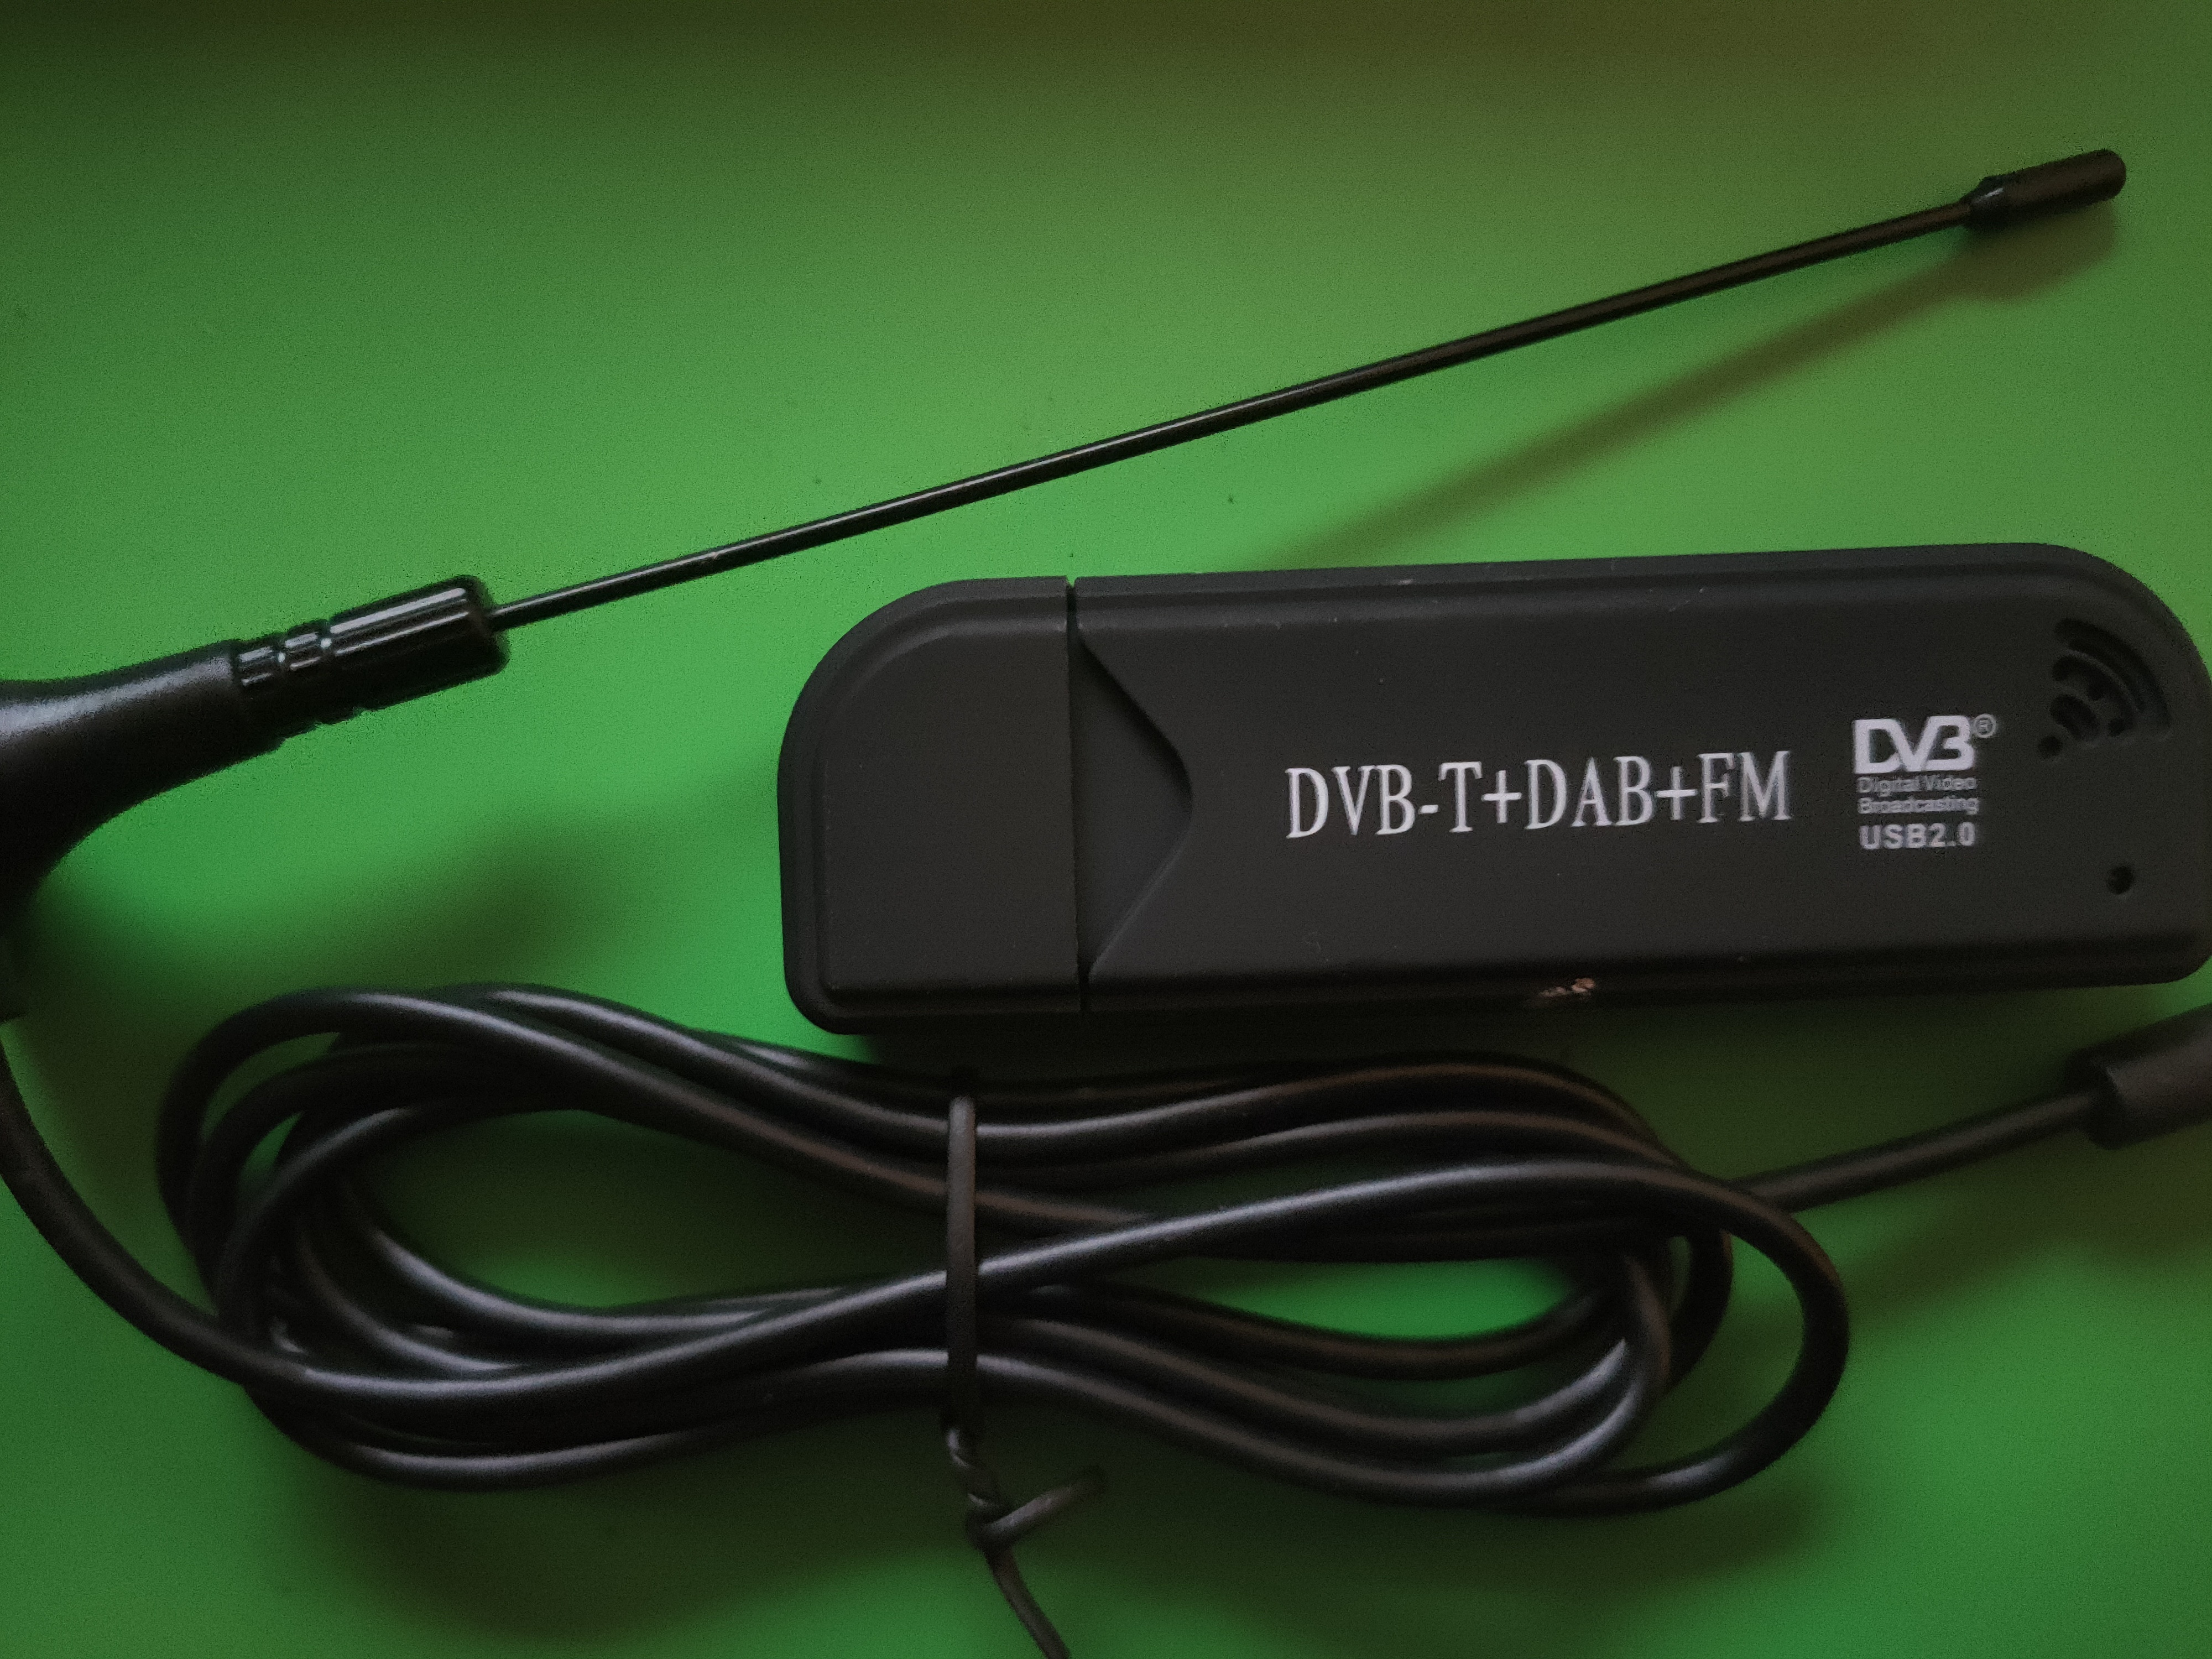
\includegraphics[width=0.5\linewidth,height=\textheight,keepaspectratio]{pictures/rtl-sdr.jpg}

La \textbf{RTL-SDR} est une clé USB basée sur le chipset
\textbf{RTL2832U} initialement conçue pour la télévision DVB-T. Le
détournement du mode \textbf{I/Q brut} a permis d'en faire le SDR le
plus populaire du monde.

Caractéristiques principales :

\begin{itemize}
\tightlist
\item
  RX uniquement
\item
  bande instantanée \textasciitilde2,4 MHz
\item
  très bon support logiciel (GNU Radio, rtl-sdr, GQRX, SDR++)
\item
  prix extrêmement bas
\end{itemize}

C'est l'outil idéal pour apprendre :

\begin{itemize}
\tightlist
\item
  ADS-B
\item
  AIS
\item
  météo satellite
\item
  analyse spectrale
\item
  écoute radio numérique
\end{itemize}

\begin{center}\rule{0.5\linewidth}{0.5pt}\end{center}

\subsubsection{ADALM-PLUTO}\label{adalm-pluto}

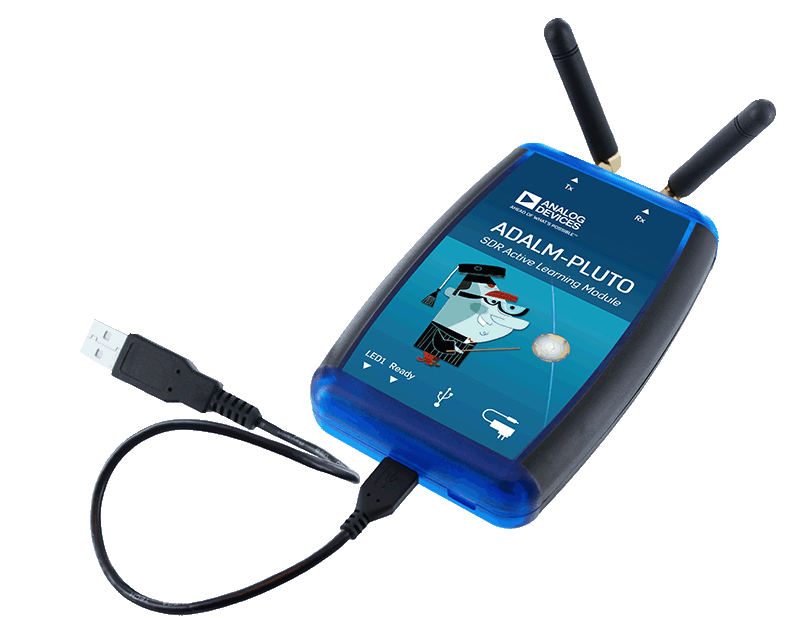
\includegraphics[width=0.5\linewidth,height=\textheight,keepaspectratio]{pictures/pluto.png}

Le \textbf{PlutoSDR} est un SDR éducatif développé par \textbf{Analog
Devices}.

Points clés :

\begin{itemize}
\tightlist
\item
  basé sur \textbf{Zynq + AD9363}
\item
  Tx/Rx full duplex
\item
  hackable (firmware modifiable)
\item
  bande instantanée 20 MHz
\end{itemize}

Très utilisé pour :

\begin{itemize}
\tightlist
\item
  4G / 5G expérimental
\item
  radar
\item
  GNURadio avancé
\end{itemize}

\begin{center}\rule{0.5\linewidth}{0.5pt}\end{center}

\subsubsection{LimeSDR Mini}\label{limesdr-mini}

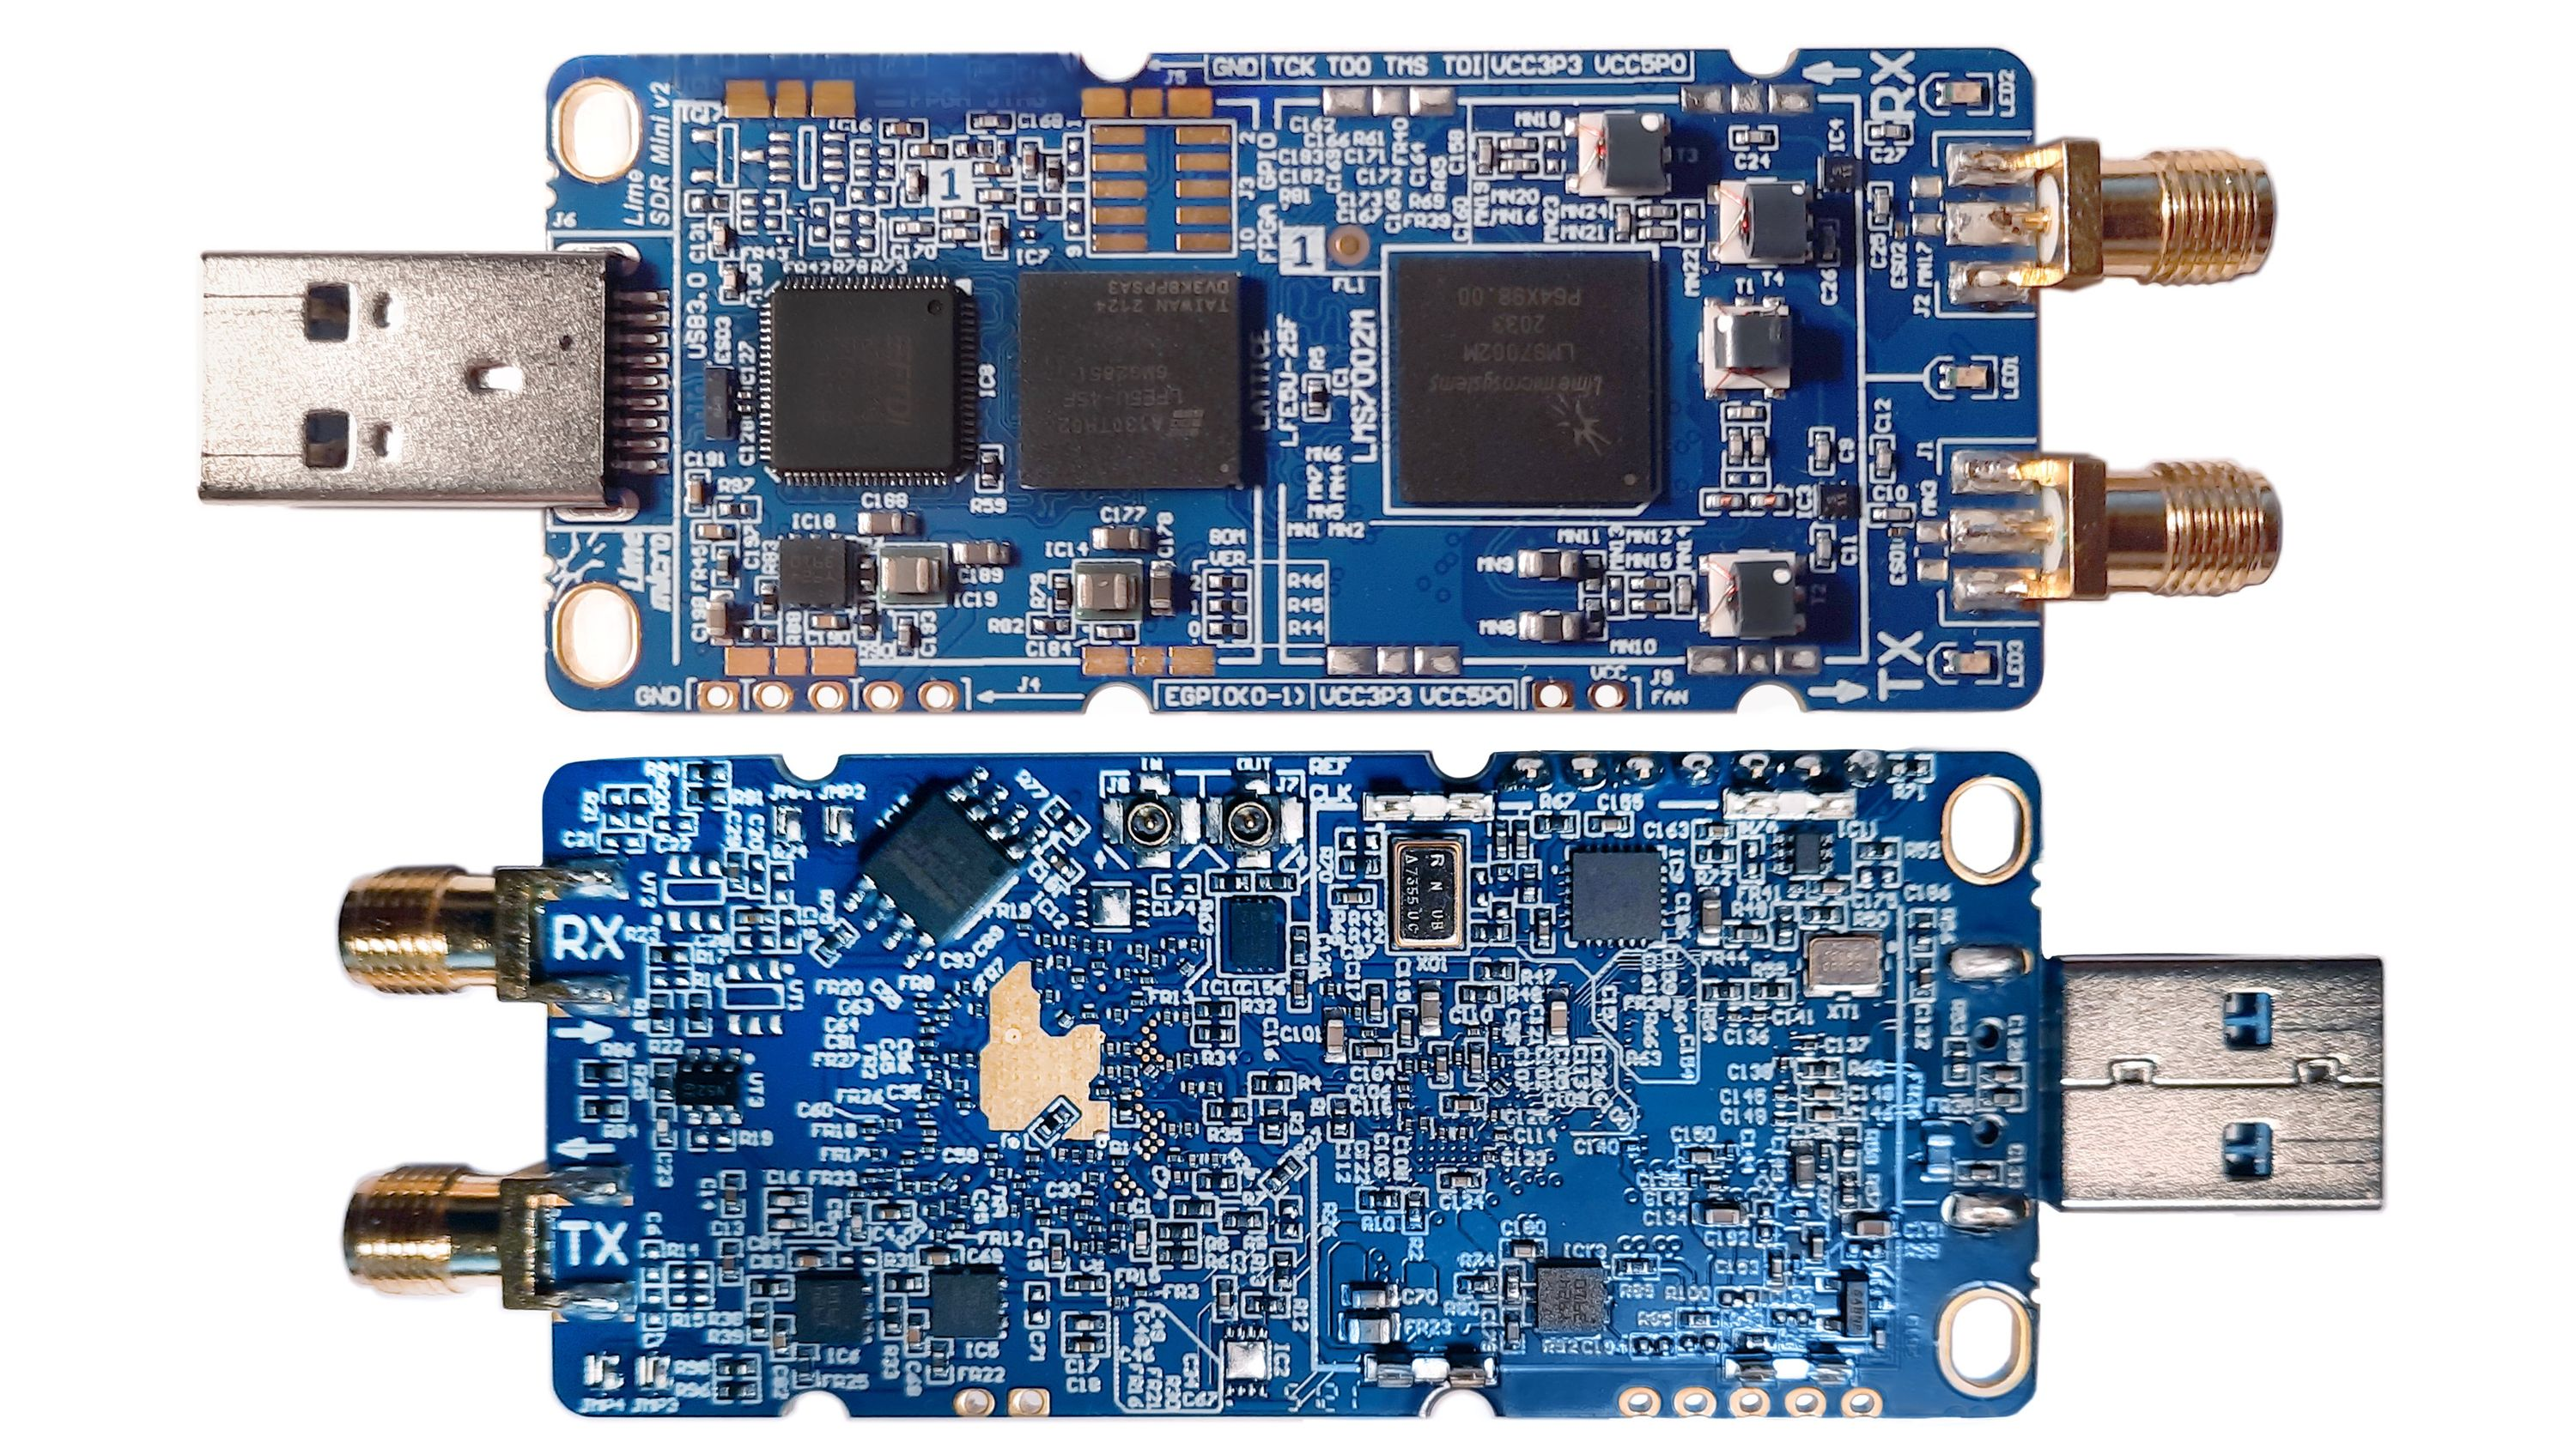
\includegraphics[width=0.5\linewidth,height=\textheight,keepaspectratio]{pictures/lime.jpg}

Le \textbf{LimeSDR Mini} utilise le transceiver \textbf{LMS7002M}.

Points forts :

\begin{itemize}
\tightlist
\item
  bande instantanée 40 MHz
\item
  FPGA ECP5 programmable
\item
  open hardware
\end{itemize}

Très apprécié pour :

\begin{itemize}
\tightlist
\item
  expérimentation LTE
\item
  SDR haute bande passante
\end{itemize}

\begin{center}\rule{0.5\linewidth}{0.5pt}\end{center}

\subsubsection{HackRF One}\label{hackrf-one}

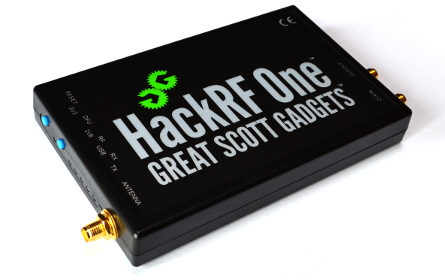
\includegraphics[width=0.5\linewidth,height=\textheight,keepaspectratio]{pictures/hackrf.jpeg}

Le \textbf{HackRF One} est probablement le SDR le plus utilisé dans la
communauté sécurité radio.

Caractéristiques :

\begin{itemize}
\tightlist
\item
  1 MHz à 6 GHz
\item
  semi-duplex
\item
  20 MHz de bande instantanée
\end{itemize}

Utilisations typiques :

\begin{itemize}
\tightlist
\item
  recherche sécurité RF
\item
  replay radio
\item
  analyse protocole
\end{itemize}

\begin{center}\rule{0.5\linewidth}{0.5pt}\end{center}

\subsubsection{BladeRF}\label{bladerf}

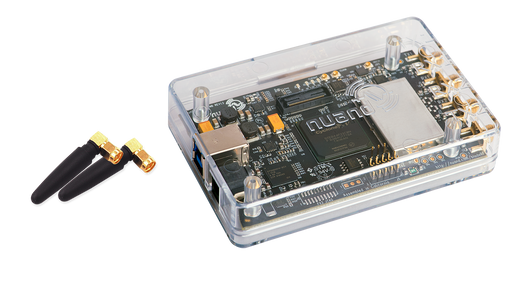
\includegraphics[width=0.5\linewidth,height=\textheight,keepaspectratio]{pictures/blade.png}

Le \textbf{BladeRF 2.0} est une plateforme SDR très puissante.

Points forts :

\begin{itemize}
\tightlist
\item
  FPGA Cyclone V
\item
  56 MHz de bande instantanée
\item
  support logiciel très mature
\end{itemize}

Utilisé pour :

\begin{itemize}
\tightlist
\item
  implémentations LTE
\item
  systèmes radio expérimentaux
\end{itemize}

\begin{center}\rule{0.5\linewidth}{0.5pt}\end{center}

\subsubsection{AntSDR}\label{antsdr}

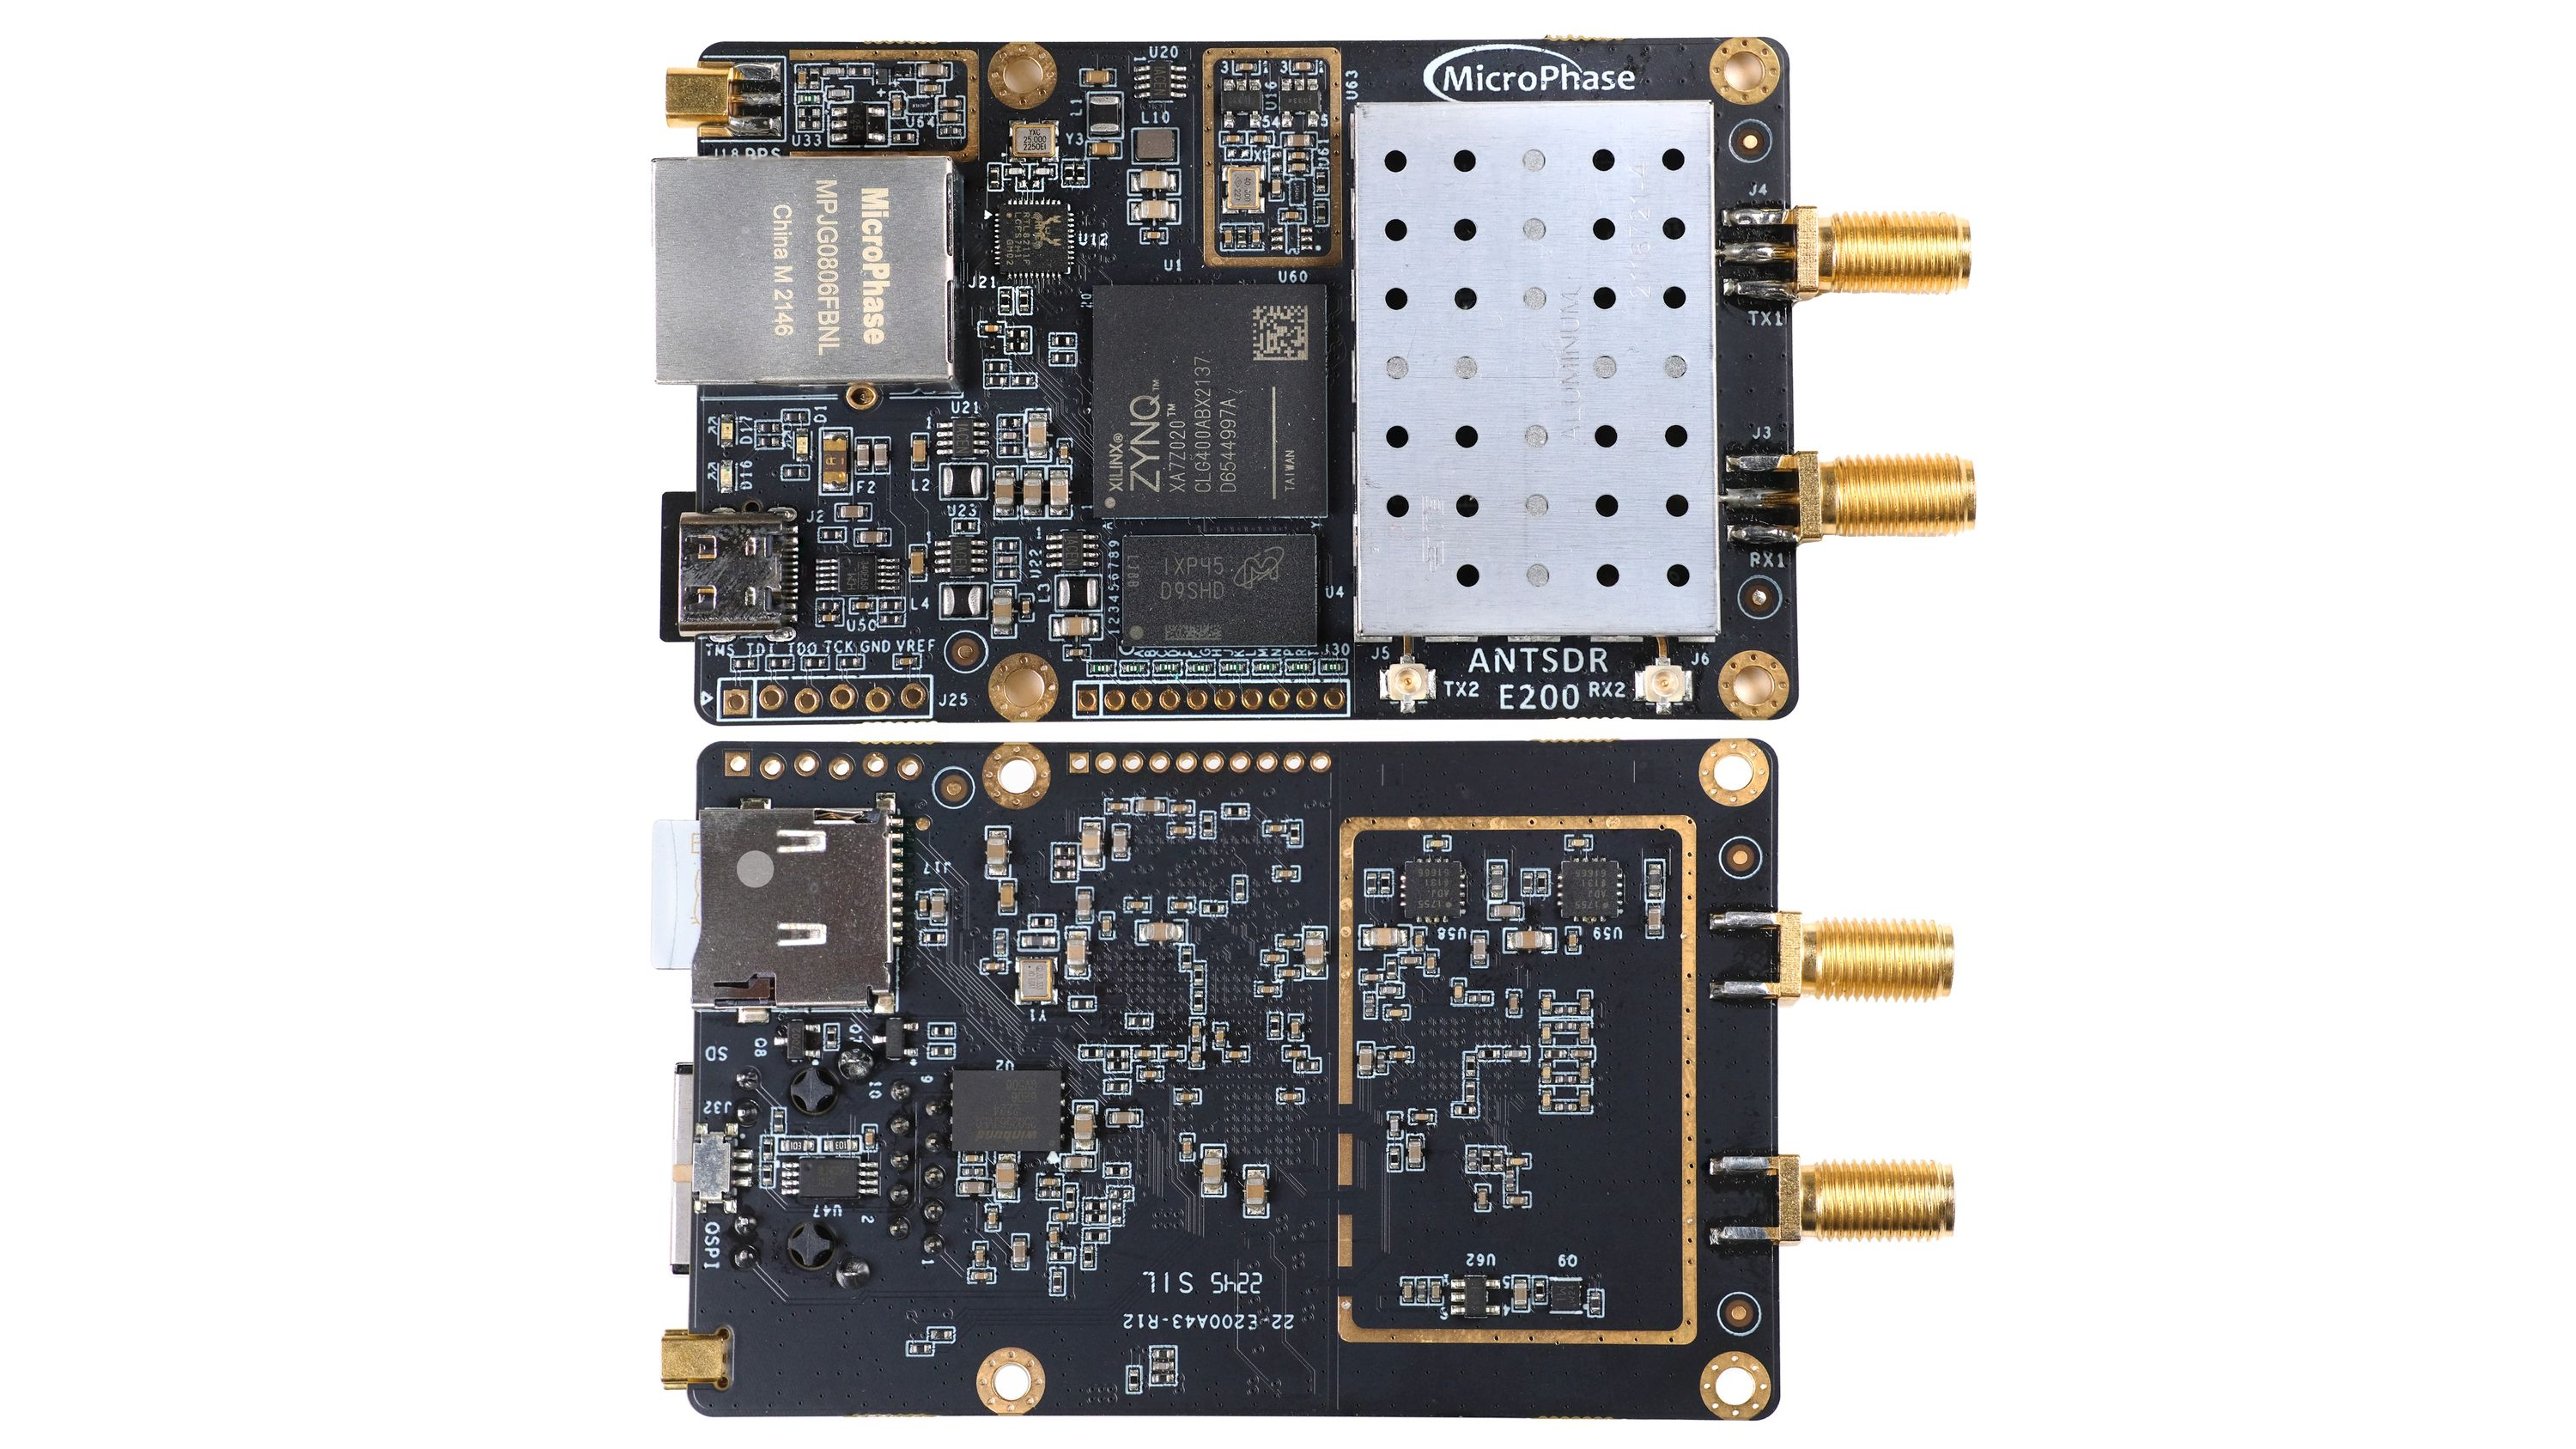
\includegraphics[width=0.5\linewidth,height=\textheight,keepaspectratio]{pictures/ant.jpg}

Les \textbf{AntSDR} sont des clones modernes des plateformes
\textbf{AD9361}.

Avantages :

\begin{itemize}
\tightlist
\item
  MIMO 2×2
\item
  Ethernet
\item
  prix très compétitif
\end{itemize}

Très intéressant pour :

\begin{itemize}
\tightlist
\item
  recherche radio avancée
\item
  systèmes multi-antennes
\end{itemize}

\begin{center}\rule{0.5\linewidth}{0.5pt}\end{center}

\subsubsection{LibreSDR}\label{libresdr}

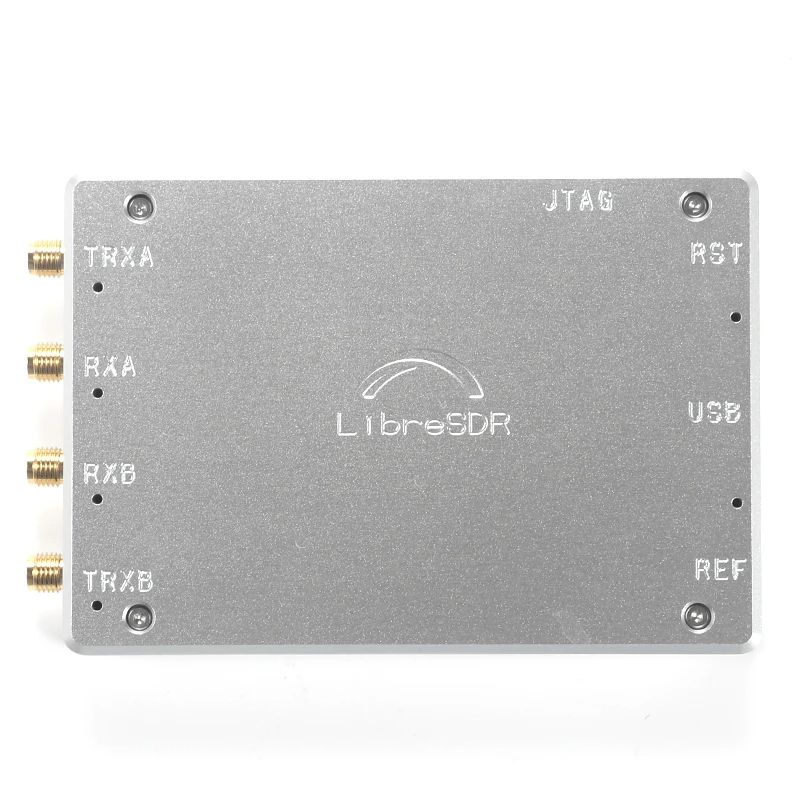
\includegraphics[width=0.5\linewidth,height=\textheight,keepaspectratio]{pictures/libre.png}

Le \textbf{LibreSDR} vise à reproduire les capacités du \textbf{USRP
B210} dans un format compact.

Caractéristiques :

\begin{itemize}
\tightlist
\item
  2×2 MIMO
\item
  USB 3
\item
  bande \textasciitilde56 MHz
\end{itemize}

Très bon rapport performance/prix.

\begin{center}\rule{0.5\linewidth}{0.5pt}\end{center}

\subsubsection{USRP B210}\label{usrp-b210}

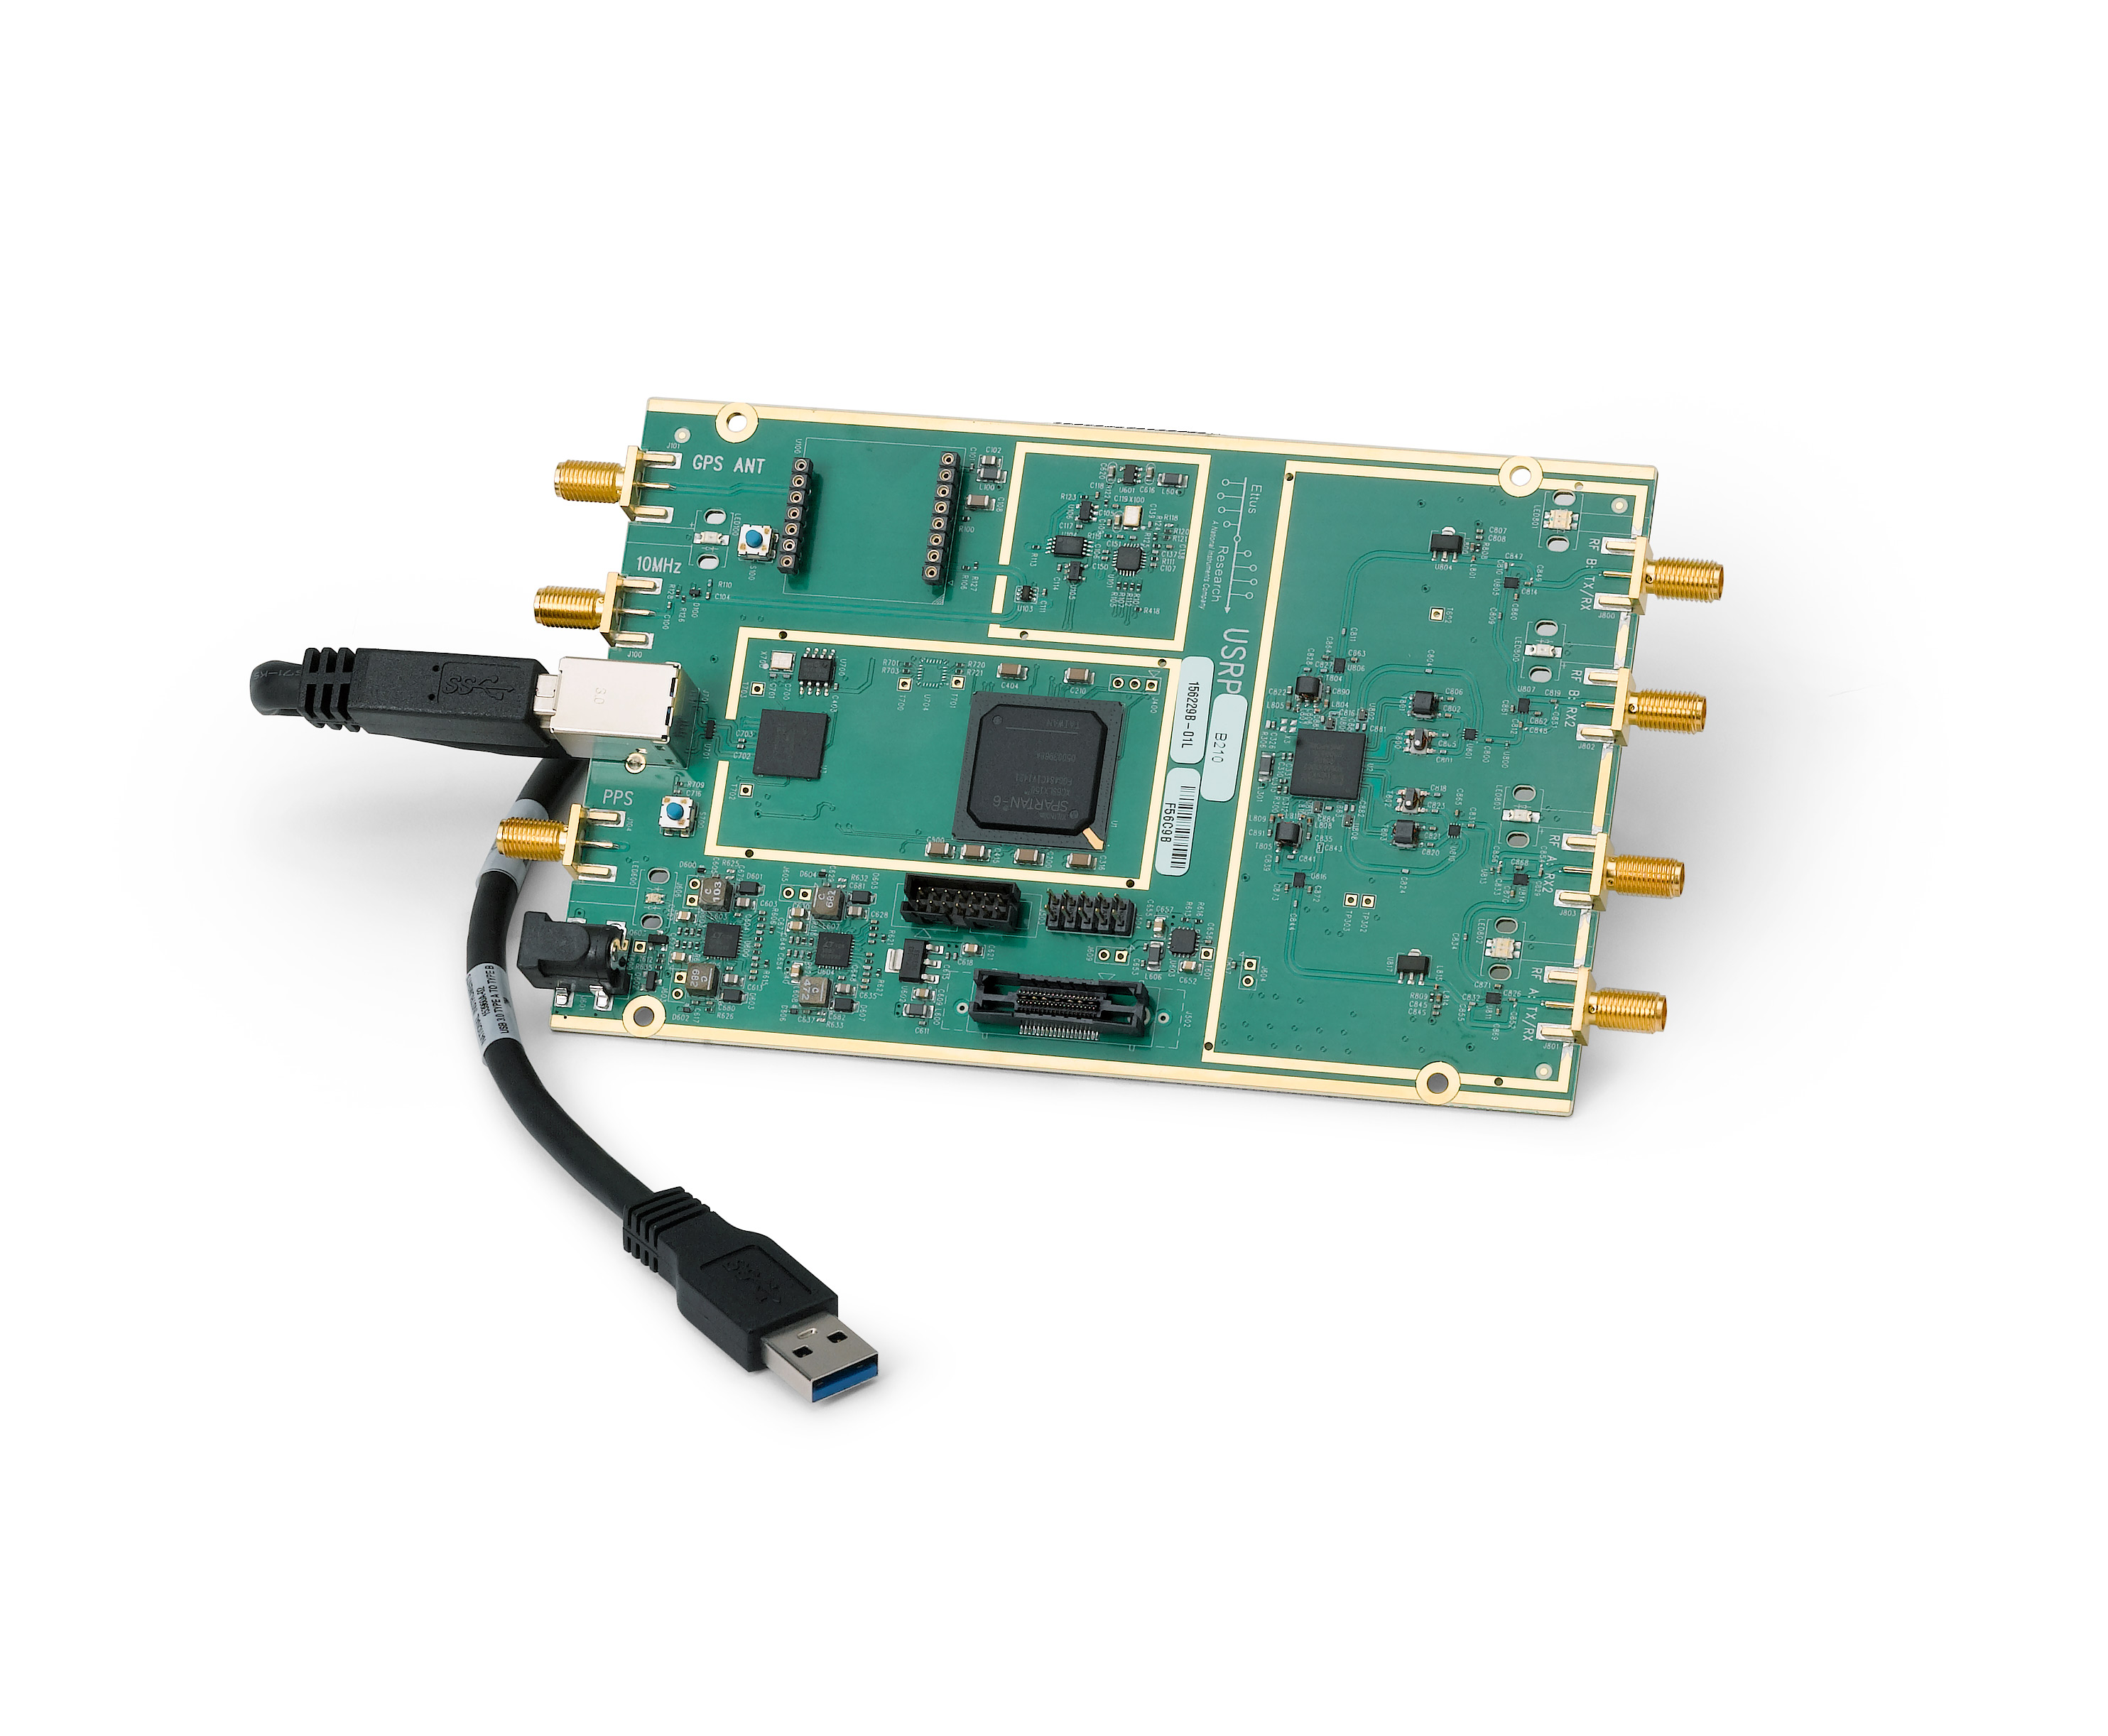
\includegraphics[width=0.5\linewidth,height=\textheight,keepaspectratio]{pictures/B210.jpg}

Le \textbf{USRP B210} est une plateforme de référence pour la recherche
SDR.

Points clés :

\begin{itemize}
\tightlist
\item
  AD9361
\item
  MIMO 2×2
\item
  UHD officiel
\end{itemize}

Très utilisé dans :

\begin{itemize}
\tightlist
\item
  laboratoires universitaires
\item
  projets GNU Radio avancés
\item
  implémentations LTE / 5G
\end{itemize}

\begin{center}\rule{0.5\linewidth}{0.5pt}\end{center}

\subsubsection{USRP X310}\label{usrp-x310}

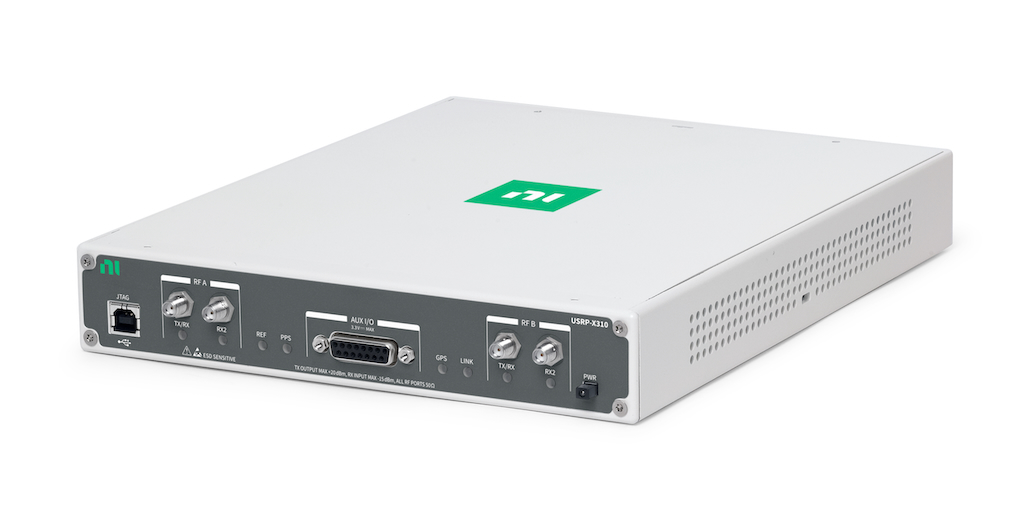
\includegraphics[width=0.5\linewidth,height=\textheight,keepaspectratio]{pictures/X310.jpeg}

Le \textbf{USRP X310} est une plateforme SDR haut de gamme.

Caractéristiques :

\begin{itemize}
\tightlist
\item
  FPGA Kintex-7
\item
  modules RF interchangeables
\item
  bande instantanée très élevée
\end{itemize}

Utilisé pour :

\begin{itemize}
\tightlist
\item
  recherche radio avancée
\item
  radar
\item
  communications expérimentales
\end{itemize}

\section{La clé RTL-SDR}\label{la-cluxe9-rtl-sdr-1}

\pandocbounded{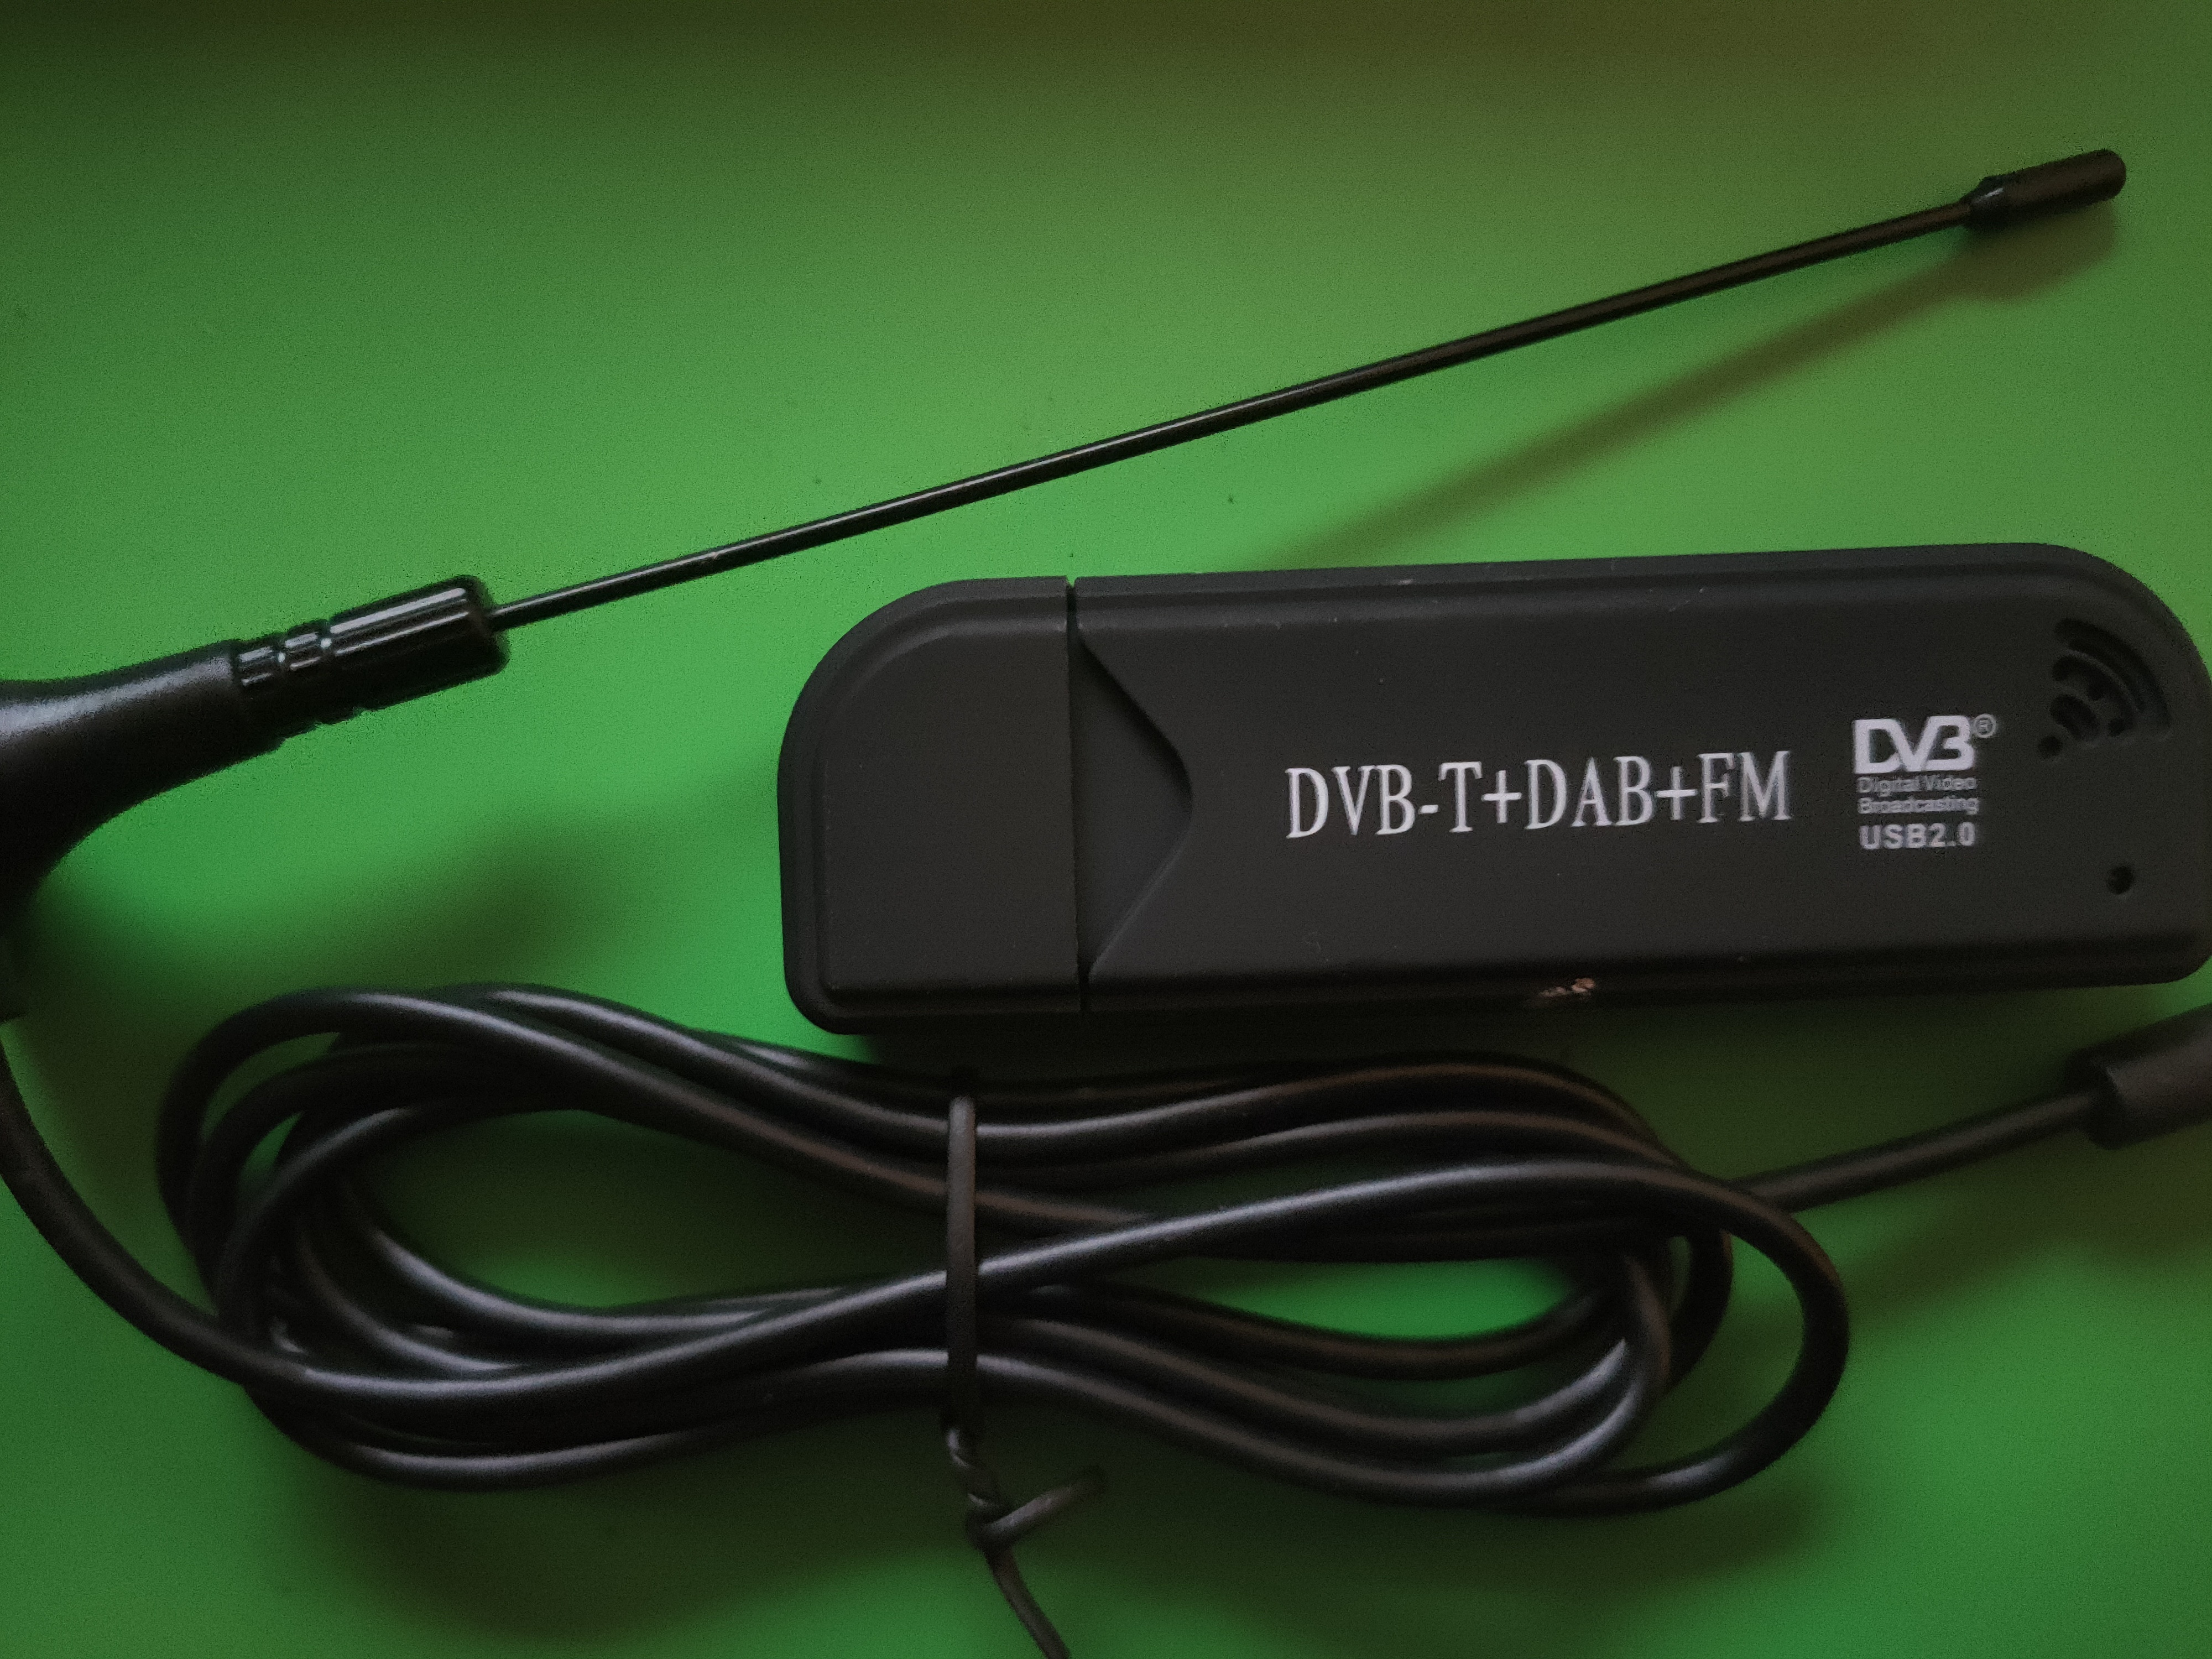
\includegraphics[keepaspectratio]{pictures/rtl.jpg}}

L'un des outils les plus accessibles pour explorer le spectre radio est
la \textbf{clé RTL-SDR}.

À l'origine, ces dispositifs étaient conçus comme de simples
\textbf{récepteurs de télévision numérique DVB-T}.\\
Cependant, il a été découvert que la puce utilisée dans ces récepteurs
permettait d'accéder directement au \textbf{flux brut du signal radio}.

Grâce à un pilote modifié, ces clés peuvent être utilisées comme
\textbf{récepteurs radio généralistes à très bas coût}.

Une clé RTL-SDR typique se compose de :

\begin{itemize}
\item
  \textbf{Un tuner radio}\\
  souvent basé sur la puce \textbf{R820T ou R860}.
\item
  \textbf{Un convertisseur analogique-numérique}\\
  intégré dans la puce \textbf{RTL2832U}.
\item
  \textbf{Une interface USB}\\
  permettant de connecter l'appareil à un ordinateur.
\end{itemize}

La clé fonctionne alors comme un \textbf{récepteur SDR (Software Defined
Radio)}.

Le principe est le suivant :

\[
\text{Onde radio} \rightarrow \text{antenne} \rightarrow \text{tuner RF} \rightarrow \text{ADC} \rightarrow \text{USB} \rightarrow \text{logiciel}
\]

La plage de fréquences typique couverte par ces clés est :

\[
24\;MHz \rightarrow 1.7\;GHz
\]

Cela permet d'observer de nombreux systèmes radio :

\begin{itemize}
\tightlist
\item
  radio \textbf{FM}
\item
  \textbf{aviation}
\item
  \textbf{satellites météo}
\item
  \textbf{AIS maritime}
\item
  \textbf{ADS-B aviation}
\item
  certains signaux \textbf{cellulaires}
\end{itemize}

Ces clés coûtent généralement \textbf{moins de 40 €}, ce qui a largement
contribué à démocratiser l'expérimentation radio.

\begin{center}\rule{0.5\linewidth}{0.5pt}\end{center}

\subsection{Installation des outils RTL-SDR sous
Ubuntu}\label{installation-des-outils-rtl-sdr-sous-ubuntu}

La première étape consiste à installer les pilotes permettant d'accéder
au matériel.

Ouvrir un terminal :

\begin{Shaded}
\begin{Highlighting}[]
\FunctionTok{sudo}\NormalTok{ apt install rtl{-}sdr}
\end{Highlighting}
\end{Shaded}

Voici une version \textbf{plus propre et fluide} que tu peux intégrer
dans ton livre.

\subsection{Configuration des permissions
RTL-SDR}\label{configuration-des-permissions-rtl-sdr}

Pour permettre à un utilisateur normal d'accéder à la clé RTL-SDR sans
utiliser \texttt{sudo}, il est nécessaire d'ajouter une règle
\textbf{udev}.

La méthode la plus simple consiste à utiliser un \textbf{here-document}
en Bash.\\
Cette technique permet d'écrire directement le contenu du fichier avec
les droits administrateur.

Exécuter la commande suivante :

\begin{Shaded}
\begin{Highlighting}[]
\FunctionTok{sudo}\NormalTok{ tee /etc/udev/rules.d/20{-}rtl{-}sdr.rules }\OperatorTok{\textgreater{}}\NormalTok{ /dev/null }\OperatorTok{\textless{}\textless{} \textquotesingle{}EOF\textquotesingle{}}
\StringTok{SUBSYSTEM=="usb", ATTRS\{idVendor\}=="0bda", ATTRS\{idProduct\}=="2832", GROUP="plugdev", MODE="0666"}
\StringTok{SUBSYSTEM=="usb", ATTRS\{idVendor\}=="0bda", ATTRS\{idProduct\}=="2838", GROUP="plugdev", MODE="0666"}
\OperatorTok{EOF}
\end{Highlighting}
\end{Shaded}

Cette règle donne aux membres du groupe \textbf{plugdev} l'accès au
périphérique RTL-SDR.

\begin{center}\rule{0.5\linewidth}{0.5pt}\end{center}

\subsection{Recharger les règles
udev}\label{recharger-les-ruxe8gles-udev}

Une fois la règle créée, il faut demander au système de recharger la
configuration :

\begin{Shaded}
\begin{Highlighting}[]
\FunctionTok{sudo}\NormalTok{ udevadm control }\AttributeTok{{-}{-}reload{-}rules}
\FunctionTok{sudo}\NormalTok{ udevadm trigger}
\end{Highlighting}
\end{Shaded}

Ensuite, \textbf{débrancher puis rebrancher la clé RTL-SDR} pour que la
règle soit appliquée.

\begin{center}\rule{0.5\linewidth}{0.5pt}\end{center}

\subsection{Vérifier que la clé
fonctionne}\label{vuxe9rifier-que-la-cluxe9-fonctionne}

Pour vérifier que le système détecte correctement la clé, utiliser
l'outil de test fourni avec les pilotes :

\begin{Shaded}
\begin{Highlighting}[]
\ExtensionTok{rtl\_test}
\end{Highlighting}
\end{Shaded}

Si tout est correctement configuré, le programme devrait afficher
quelque chose comme :

\begin{Shaded}
\begin{Highlighting}[]
\NormalTok{Found 1 device(s):}
\NormalTok{Realtek RTL2838UHIDIR}
\end{Highlighting}
\end{Shaded}

Cela indique que la clé est correctement reconnue par le système et
prête à être utilisée par les logiciels SDR.

\subsection{Vérifier que la clé est
détectée}\label{vuxe9rifier-que-la-cluxe9-est-duxe9tectuxe9e}

Brancher la clé USB puis exécuter :

\begin{Shaded}
\begin{Highlighting}[]
\ExtensionTok{rtl\_test}
\end{Highlighting}
\end{Shaded}

Si l'installation fonctionne, le programme affiche quelque chose comme :

\begin{verbatim}
Found 1 device(s):
Realtek RTL2838UHIDIR
\end{verbatim}

Le programme commence ensuite à tester la réception du signal.

Pour arrêter le test :

\begin{verbatim}
CTRL + C
\end{verbatim}

Si ce message apparaît, la clé est correctement reconnue par le système.

\begin{center}\rule{0.5\linewidth}{0.5pt}\end{center}

\section{Installation de GQRX}\label{installation-de-gqrx}

Pour visualiser les signaux radio, on utilise un logiciel appelé
\textbf{GQRX}.

GQRX est une interface graphique permettant de :

\begin{itemize}
\tightlist
\item
  observer le \textbf{spectre radio}
\item
  syntoniser une \textbf{fréquence}
\item
  écouter les \textbf{signaux analogiques}
\item
  analyser les transmissions
\end{itemize}

Installer GQRX avec :

\begin{Shaded}
\begin{Highlighting}[]
\FunctionTok{sudo}\NormalTok{ apt install gqrx{-}sdr}
\end{Highlighting}
\end{Shaded}

\begin{center}\rule{0.5\linewidth}{0.5pt}\end{center}

\section{Lancer GQRX}\label{lancer-gqrx}

Démarrer le programme :

\begin{Shaded}
\begin{Highlighting}[]
\ExtensionTok{gqrx}
\end{Highlighting}
\end{Shaded}

Lors du premier lancement, une fenêtre de configuration apparaît.

Paramètres recommandés :

\begin{itemize}
\tightlist
\item
  \textbf{Device} : RTL-SDR
\item
  \textbf{Sample rate} : 2.4 MS/s
\item
  \textbf{Input rate} : automatique
\end{itemize}

Cliquer sur \textbf{Start DSP}.

Le logiciel affiche alors :

\begin{itemize}
\tightlist
\item
  un \textbf{spectre radio}
\item
  une \textbf{cascade (waterfall)} des signaux reçus
\end{itemize}

Chaque pic visible dans le spectre correspond à \textbf{une transmission
radio}.

\begin{center}\rule{0.5\linewidth}{0.5pt}\end{center}

\begin{enumerate}
\def\labelenumi{\arabic{enumi}.}
\setcounter{enumi}{2}
\tightlist
\item
  ajuster le \textbf{gain} si nécessaire
\end{enumerate}

Si une station radio est présente, vous devriez \textbf{entendre la
musique} immédiatement.

Cette expérience simple montre un point essentiel :

\textbf{le spectre radio est rempli de signaux invisibles que l'on peut
observer avec une simple clé SDR et un ordinateur.}

Dans les chapitres suivants, nous utiliserons ces outils pour
\textbf{explorer différents systèmes radio et protocoles de
communication}.

la \textbf{clé RTL-SDR} est un accident technologique fascinant.

Les ingénieurs de Realtek n'ont jamais prévu que cette puce devienne un
\textbf{instrument scientifique mondial}.

Mais en exposant le \textbf{flux I/Q brut}, ils ont créé sans le vouloir
l'un des outils les plus utilisés pour :

\begin{itemize}
\tightlist
\item
  la \textbf{radio amateur}
\item
  la \textbf{recherche en télécom}
\item
  l'\textbf{analyse de protocoles radio}
\item
  la \textbf{sécurité sans fil}
\end{itemize}

Un détail intéressant de l'histoire de ces clés est qu'elles
\textbf{n'étaient pas conçues à l'origine pour être des récepteurs SDR}.

Le circuit \textbf{RTL2832U}, fabriqué par Realtek, était destiné aux
récepteurs \textbf{DVB-T (télévision numérique)}. Cependant, les
ingénieurs avaient laissé accessible un \textbf{mode interne permettant
de récupérer le flux IQ brut} utilisé pour la démodulation.

Vers \textbf{2012}, des chercheurs et radioamateurs ont découvert ce
mode et ont développé des pilotes permettant d'y accéder.

Cette découverte a transformé un simple récepteur TV à bas coût en
\textbf{récepteur radio large bande programmable}, ouvrant la porte à
une démocratisation massive de l'expérimentation radio.

Aujourd'hui, une clé RTL-SDR coûtant quelques dizaines d'euros permet
d'explorer un spectre radio qui nécessitait autrefois \textbf{des
analyseurs de spectre professionnels coûtant plusieurs dizaines de
milliers d'euros}.

\section{Première expérience : écouter la radio
FM}\label{premiuxe8re-expuxe9rience-uxe9couter-la-radio-fm}

Pour tester la réception :

\begin{enumerate}
\def\labelenumi{\arabic{enumi}.}
\tightlist
\item
  régler la fréquence autour de
\end{enumerate}

\begin{verbatim}
100 MHz
\end{verbatim}

\begin{enumerate}
\def\labelenumi{\arabic{enumi}.}
\setcounter{enumi}{1}
\tightlist
\item
  choisir le mode :
\end{enumerate}

\begin{verbatim}
WFM (Wide FM)
\end{verbatim}

\pandocbounded{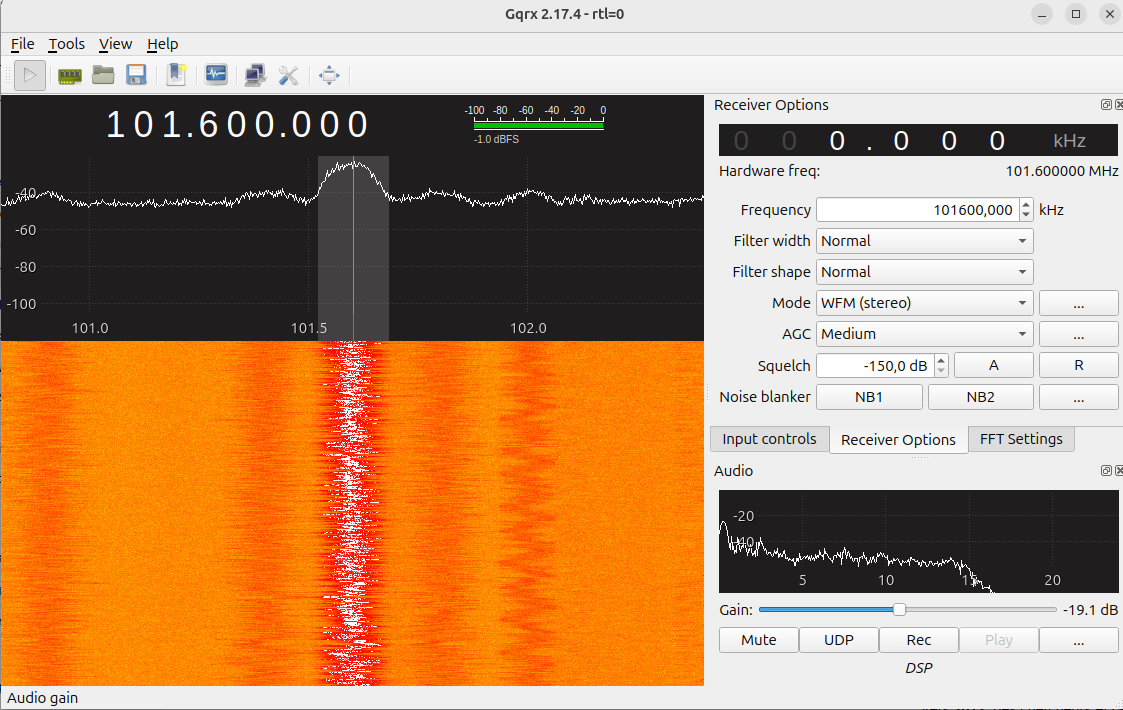
\includegraphics[keepaspectratio]{pictures/gqrx.png}}

\section{Sniffing GSM passif}\label{sniffing-gsm-passif}

\subsection{Installation de gr-gsm}\label{installation-de-gr-gsm}

Le projet \textbf{gr-gsm} est un ensemble de modules développés pour
\textbf{GNU Radio} permettant d'analyser et de décoder les signaux des
réseaux \textbf{GSM}.

Il est utilisé pour :

\begin{itemize}
\tightlist
\item
  observer les \textbf{canaux GSM}
\item
  analyser les \textbf{messages de signalisation}
\item
  étudier le fonctionnement des réseaux mobiles
\end{itemize}

Le projet est disponible sur GitHub :

\url{https://github.com/bkerler/gr-gsm}

\subsubsection{Dépendances
nécessaires}\label{duxe9pendances-nuxe9cessaires}

Avant d'installer gr-gsm, certaines bibliothèques doivent être
installées.

Exécuter :

\begin{Shaded}
\begin{Highlighting}[]
\FunctionTok{sudo}\NormalTok{ apt update}
\end{Highlighting}
\end{Shaded}

Puis installer les dépendances principales :

\begin{Shaded}
\begin{Highlighting}[]
\FunctionTok{sudo}\NormalTok{ apt install gr{-}osmosdr libosmocore{-}dev}
\end{Highlighting}
\end{Shaded}

Ces deux paquets sont essentiels.

\begin{itemize}
\item
  \textbf{gr-osmosdr}

  Ce module permet à \textbf{GNU Radio} d'accéder aux périphériques SDR.

  Il supporte de nombreux matériels :

  \begin{itemize}
  \tightlist
  \item
    RTL-SDR
  \item
    HackRF
  \item
    USRP
  \item
    LimeSDR
  \item
    Airspy
  \end{itemize}

  Il agit comme une \textbf{interface entre le matériel radio et GNU
  Radio}.
\item
  \textbf{libosmocore-dev}

  Cette bibliothèque fait partie de l'écosystème \textbf{Osmocom}.

  Elle contient des fonctions utilisées dans de nombreux projets télécom
  :

  \begin{itemize}
  \tightlist
  \item
    gestion de protocoles GSM
  \item
    structures de messages
  \item
    outils de décodage
  \end{itemize}

  Le paquet \texttt{-dev} contient les \textbf{fichiers nécessaires à la
  compilation} des logiciels utilisant cette bibliothèque.
\end{itemize}

\subsubsection{Installation de gr-gsm}\label{installation-de-gr-gsm-1}

Une fois les dépendances installées, cloner le dépôt :

\begin{Shaded}
\begin{Highlighting}[]
\FunctionTok{git}\NormalTok{ clone https://github.com/bkerler/gr{-}gsm.git}
\BuiltInTok{cd}\NormalTok{ gr{-}gsm}
\end{Highlighting}
\end{Shaded}

Créer ensuite un dossier de compilation :

\begin{Shaded}
\begin{Highlighting}[]
\FunctionTok{mkdir}\NormalTok{ build}
\BuiltInTok{cd}\NormalTok{ build}
\end{Highlighting}
\end{Shaded}

Configurer la compilation :

\begin{Shaded}
\begin{Highlighting}[]
\FunctionTok{cmake}\NormalTok{ ..}
\end{Highlighting}
\end{Shaded}

Compiler le logiciel :

\begin{Shaded}
\begin{Highlighting}[]
\FunctionTok{make}
\end{Highlighting}
\end{Shaded}

Installer les modules :

\begin{Shaded}
\begin{Highlighting}[]
\FunctionTok{sudo}\NormalTok{ make install}
\end{Highlighting}
\end{Shaded}

Enfin, mettre à jour le cache des bibliothèques :

\begin{Shaded}
\begin{Highlighting}[]
\FunctionTok{sudo}\NormalTok{ ldconfig}
\end{Highlighting}
\end{Shaded}

\subsubsection{Vérifier l'installation}\label{vuxe9rifier-linstallation}

Après l'installation, plusieurs outils doivent être disponibles.

Par exemple :

\begin{Shaded}
\begin{Highlighting}[]
\ExtensionTok{grgsm\_livemon}
\end{Highlighting}
\end{Shaded}

Cet outil permet d'observer en temps réel un canal GSM capté par une
\textbf{clé RTL-SDR}.

Si l'installation est correcte, le programme devrait démarrer et
afficher les messages GSM décodés.

Avec :

clé RTL-SDR + GNU Radio + gr-gsm

\pandocbounded{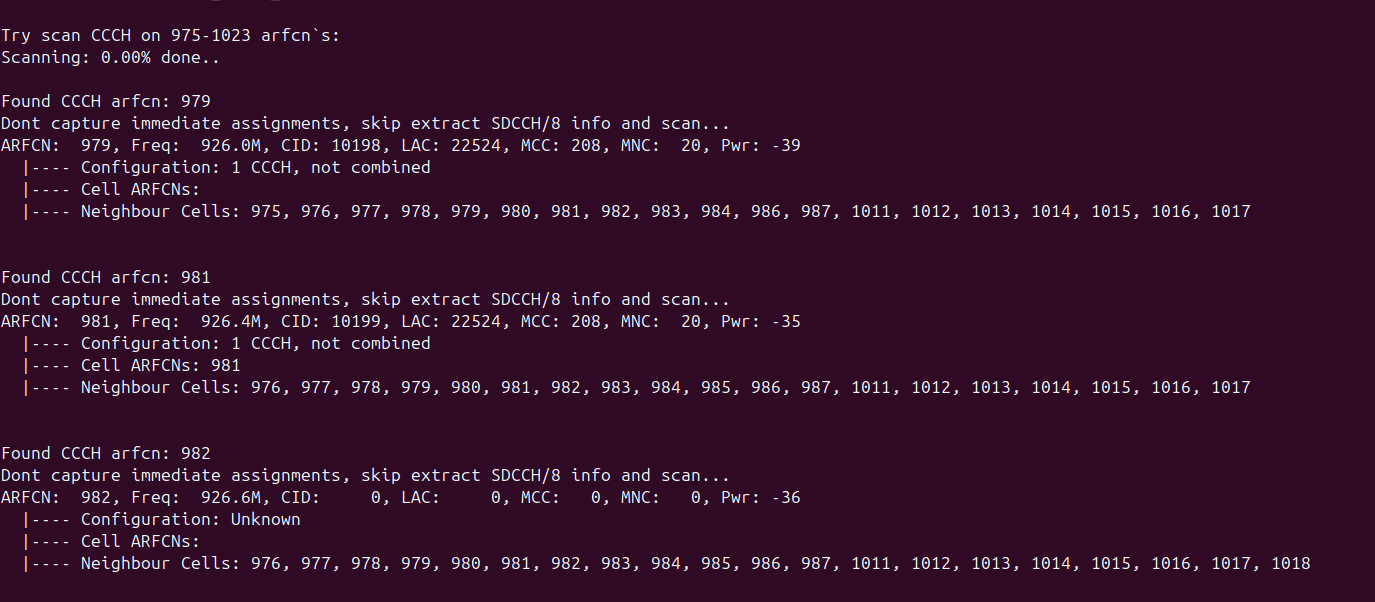
\includegraphics[keepaspectratio]{pictures/grgsm_scan.png}}

\section{Réseaux mobiles}\label{ruxe9seaux-mobiles}

\subsection{Objectif de cet ouvrage}\label{objectif-de-cet-ouvrage}

L'objectif de ce livre est d'expliquer le fonctionnement interne des
réseaux mobiles en partant des bases radio jusqu'aux mécanismes de
signalisation qui orchestrent leur fonctionnement.

À travers l'étude d'un laboratoire reproductible, nous analyserons :

\begin{itemize}
\tightlist
\item
  l'architecture des réseaux GSM
\item
  les protocoles de signalisation utilisés par les opérateurs
\item
  les interactions entre réseaux mobiles
\item
  les mécanismes historiques qui ont façonné l'infrastructure actuelle
\end{itemize}

Cette approche permet de comprendre non seulement comment ces réseaux
fonctionnent, mais aussi pourquoi ils ont été conçus de cette manière.

Les chapitres suivants exploreront progressivement les différentes
couches du système, en commençant par les bases du GSM et de la
signalisation SS7, avant d'aborder les architectures plus modernes et
les implications en matière de sécurité.

\subsection{Présentation}\label{pruxe9sentation}

Ce guide décrit l'installation modulaire d'une infrastructure
\textbf{EGPRS} (GPRS/EDGE) basée sur Osmocom et SDR (USRP, BladeRF).\\
Chaque chapitre détaille un module, son rôle, ses dépendances et
options.\\
Tout peut être scripté pour une intégration Dockerfile ou un déploiement
manuel sur Debian/Ubuntu 22.04+.

\begin{center}\rule{0.5\linewidth}{0.5pt}\end{center}

\subsection{Dépendances système}\label{duxe9pendances-systuxe8me}

Commencez par installer tous les outils de build essentiels,
bibliothèques, Python et utilitaires de debug : - Compilation :
\texttt{gcc}, \texttt{g++}, \texttt{make}, \texttt{cmake},
\texttt{autoconf}, \texttt{automake}, \texttt{libtool}, etc. - Libs
système : \texttt{libusb-1.0-0-dev}, \texttt{libedit-dev},
\texttt{libfftw3-dev}, \texttt{liburing-dev}, \ldots{} - Dev Python :
\texttt{python3-dev}, \texttt{python3-pip}, \texttt{python3-numpy},
\texttt{python3-mako}, \texttt{python3-lxml}, \texttt{python3-six},
\ldots{} - Outils additionnels : \texttt{nano}, \texttt{git},
\texttt{wget}, \texttt{curl}, \texttt{tmux}, \texttt{doxygen},
\texttt{ethtool}, etc.

\textbf{Commande d'installation :}

\begin{Shaded}
\begin{Highlighting}[]
\ExtensionTok{apt}\NormalTok{ update}
\ExtensionTok{apt}\NormalTok{ install }\AttributeTok{{-}y} \OperatorTok{\textless{}}\NormalTok{tous{-}les{-}paquets{-}listés}\OperatorTok{\textgreater{}}
\end{Highlighting}
\end{Shaded}

\begin{center}\rule{0.5\linewidth}{0.5pt}\end{center}

\subsection{OsmocomBB}\label{osmocombb}

\textbf{OsmocomBB} (Osmocom Baseband) est un projet open source qui
implémente une pile GSM ``baseband'' pour certains téléphones Motorola
et des configurations SDR.

\subsubsection{Qu'est-ce qu'OsmocomBB\,?}\label{quest-ce-quosmocombb}

\begin{itemize}
\tightlist
\item
  \textbf{Pile protocolaire GSM côté mobile (MS, mobile station)}
\item
  Remplace le firmware d'origine pour donner accès aux couches GSM
  1/2/3, journalisation des protocoles, sniffing et tests
\item
  Utilisations\,: analyse, tests de sécurité, recherche académique, IMSI
  catchers, fuzzing radio
\end{itemize}

\subsubsection{Architecture}\label{architecture}

\begin{itemize}
\tightlist
\item
  \textbf{host/osmocon}\,: Outil de chargement du firmware sur les
  appareils compatibles
\item
  \textbf{src/host/layer23}\,: Pile GSM s'exécutant sur le PC (appels,
  SMS, sniffing, capture de bursts, etc.)
\item
  \textbf{firmware/}\,: Code baseband à flasher sur les téléphones
  compatibles
\end{itemize}

\subsubsection{Matériel supporté}\label{matuxe9riel-supportuxe9}

\begin{itemize}
\tightlist
\item
  \textbf{Série Motorola C1xx (C123, C118, C155, etc.)}
\item
  Certains autres modèles à chipset ``Calypso''
\end{itemize}

\subsubsection{Cas d'usage \& limitations}\label{cas-dusage-limitations}

\begin{itemize}
\tightlist
\item
  Peut se connecter à une vraie cellule 2G ou à une BTS Osmocom
  (osmo-bts-trx)
\item
  Limité à la 2G pure (pas de support 3G/4G)
\item
  \textbf{Attention\,:} Émettre sans licence est illégal\,!\\
  N'utilisez que pour la recherche ou en environnement contrôlé.
\end{itemize}

\subsubsection{Liens utiles}\label{liens-utiles}

\begin{itemize}
\tightlist
\item
  \href{https://github.com/osmocom/osmocom-bb}{Dépôt GitHub OsmocomBB}
\item
  \href{https://osmocom.org/projects/baseband/wiki/OsmocomBB}{Wiki
  officiel}
\item
  \href{https://www.lafabriquedunet.fr/blog/osmocombb-guide/}{Guide
  d'installation (FR)}
\end{itemize}

\begin{center}\rule{0.5\linewidth}{0.5pt}\end{center}

\textbf{Pour SDR\,:} Un projet expérimental existe pour connecter
OsmocomBB à un SDR (BladeRF, HackRF, etc.) via l'interface ``virtual
layer1''.

\subsection{OsmocomBB Mobile (MS) -- Installation rapide Ubuntu
24.04}\label{osmocombb-mobile-ms-installation-rapide-ubuntu-24.04}

\subsubsection{Prérequis}\label{pruxe9requis}

\begin{itemize}
\item
  \textbf{Matériel\,:}

  \begin{itemize}
  \tightlist
  \item
    Motorola C1xx (C115/C118/C123/C155, etc., baseband Calypso)
  \item
    Câble USB-série 2.5\,mm (PL2303 ou FTDI)
  \end{itemize}
\item
  \textbf{Système\,:}

  \begin{itemize}
  \tightlist
  \item
    Ubuntu 24.04 x86\_64 (natif ou VM)
  \item
    Accès internet + droits sudo/root
  \end{itemize}
\end{itemize}

\begin{center}\rule{0.5\linewidth}{0.5pt}\end{center}

\subsubsection{Installer les
dépendances}\label{installer-les-duxe9pendances}

\begin{Shaded}
\begin{Highlighting}[]
\FunctionTok{sudo}\NormalTok{ apt update}
\FunctionTok{sudo}\NormalTok{ apt install }\AttributeTok{{-}y} \DataTypeTok{\textbackslash{}}
\NormalTok{  build{-}essential git cmake pkg{-}config autoconf automake libtool shtool }\DataTypeTok{\textbackslash{}}
\NormalTok{  bison flex libtalloc{-}dev libpcsclite{-}dev zlib1g{-}dev libmpfr{-}dev libmpc{-}dev }\DataTypeTok{\textbackslash{}}
\NormalTok{  libgmp{-}dev libncurses5{-}dev libncursesw5{-}dev libsofia{-}sip{-}ua{-}dev libxml2{-}dev }\DataTypeTok{\textbackslash{}}
\NormalTok{  libfftw3{-}dev libgnutls28{-}dev libssl{-}dev python3 python3{-}pip }\DataTypeTok{\textbackslash{}}
\NormalTok{  alsa{-}oss lemon libtinfo{-}dev}
\end{Highlighting}
\end{Shaded}

\begin{center}\rule{0.5\linewidth}{0.5pt}\end{center}

\subsubsection{Installer la toolchain ARM (cross-compile
Calypso)}\label{installer-la-toolchain-arm-cross-compile-calypso}

\begin{Shaded}
\begin{Highlighting}[]
\BuiltInTok{cd}\NormalTok{ /opt}
\FunctionTok{sudo}\NormalTok{ wget https://downloads.osmocom.org/binaries/toolchain/arm{-}2021.03.tar.bz2}
\FunctionTok{sudo}\NormalTok{ tar }\AttributeTok{{-}xjf}\NormalTok{ arm{-}2021.03.tar.bz2}
\BuiltInTok{export} \VariableTok{PATH}\OperatorTok{=}\VariableTok{$PATH}\NormalTok{:/opt/arm{-}2021.03/bin}
\end{Highlighting}
\end{Shaded}

\begin{quote}
\emph{(Ajoute ce dernier export à ton \texttt{\textasciitilde{}/.bashrc}
pour qu'il soit permanent)}
\end{quote}

\begin{center}\rule{0.5\linewidth}{0.5pt}\end{center}

\subsubsection{Cloner et compiler
OsmocomBB}\label{cloner-et-compiler-osmocombb}

\begin{Shaded}
\begin{Highlighting}[]
\FunctionTok{git}\NormalTok{ clone https://github.com/osmocom/osmocom{-}bb.git}
\BuiltInTok{cd}\NormalTok{ osmocom{-}bb/src}
\ExtensionTok{autoreconf} \AttributeTok{{-}i}
\BuiltInTok{export} \VariableTok{PATH}\OperatorTok{=}\VariableTok{$PATH}\NormalTok{:/opt/arm{-}2021.03/bin}
\ExtensionTok{./configure}
\FunctionTok{make} \AttributeTok{{-}j}\VariableTok{$(}\FunctionTok{nproc}\VariableTok{)}
\end{Highlighting}
\end{Shaded}

\begin{center}\rule{0.5\linewidth}{0.5pt}\end{center}

\subsubsection{Flasher le firmware Mobile (Compal/C123
etc.)}\label{flasher-le-firmware-mobile-compalc123-etc.}

\begin{enumerate}
\def\labelenumi{\arabic{enumi}.}
\item
  \textbf{Branche le téléphone via le câble USB-série (sans la
  batterie).}
\item
  \textbf{Dans un terminal\,:}
\end{enumerate}

\begin{Shaded}
\begin{Highlighting}[]
\BuiltInTok{cd}\NormalTok{ host/osmocon}
\FunctionTok{sudo}\NormalTok{ ./osmocon }\AttributeTok{{-}m}\NormalTok{ c123xor }\AttributeTok{{-}p}\NormalTok{ /dev/ttyUSB0 }\AttributeTok{{-}c}\NormalTok{ ../../target/firmware/board/compal\_e88/hello\_world.highram.bin}
\CommentTok{\# (optionnel : tester hello\_world)}
\end{Highlighting}
\end{Shaded}

\begin{enumerate}
\def\labelenumi{\arabic{enumi}.}
\setcounter{enumi}{2}
\tightlist
\item
  \textbf{Pour le firmware mobile complet\,:}
\end{enumerate}

\begin{Shaded}
\begin{Highlighting}[]
\FunctionTok{sudo}\NormalTok{ ./osmocon }\AttributeTok{{-}m}\NormalTok{ c123xor }\AttributeTok{{-}p}\NormalTok{ /dev/ttyUSB0 }\AttributeTok{{-}c}\NormalTok{ ../../target/firmware/board/compal\_e88/layer1.highram.bin}
\end{Highlighting}
\end{Shaded}

\begin{enumerate}
\def\labelenumi{\arabic{enumi}.}
\setcounter{enumi}{3}
\tightlist
\item
  \textbf{Dans un autre terminal\,:}
\end{enumerate}

\begin{Shaded}
\begin{Highlighting}[]
\BuiltInTok{cd}\NormalTok{ host/layer23/src/mobile}
\ExtensionTok{./mobile}
\end{Highlighting}
\end{Shaded}

\begin{center}\rule{0.5\linewidth}{0.5pt}\end{center}

\subsubsection{\texorpdfstring{Configurer \texttt{mobile.cfg} (SIM,
PLMN, log,
etc.)}{Configurer mobile.cfg (SIM, PLMN, log, etc.)}}\label{configurer-mobile.cfg-sim-plmn-log-etc.}

Crée/édite le fichier \texttt{mobile.cfg} (exemple dans
\texttt{osmocom-bb/src/host/layer23/src/mobile/})\,:

\begin{Shaded}
\begin{Highlighting}[]
\DataTypeTok{log gsmtap 127.0.0.1}
\DataTypeTok{log stderr}
\DataTypeTok{hlr}
\DataTypeTok{  subscriber{-}list subscriber\_list.csv}
\DataTypeTok{sim}
\DataTypeTok{  driver sysmo}
\end{Highlighting}
\end{Shaded}

\emph{(Adapte la section SIM si tu utilises une vraie SIM ou une ``test
SIM'')}

\begin{center}\rule{0.5\linewidth}{0.5pt}\end{center}

\subsubsection{Lancer OsmocomBB Mobile}\label{lancer-osmocombb-mobile}

\begin{Shaded}
\begin{Highlighting}[]
\CommentTok{\# Dans host/layer23/src/mobile/}
\ExtensionTok{./mobile} \AttributeTok{{-}c}\NormalTok{ mobile.cfg}
\end{Highlighting}
\end{Shaded}

\begin{itemize}
\tightlist
\item
  Le téléphone démarre, tente de s'enregistrer sur le réseau configuré.
\item
  Regarde les logs\,: tu dois voir ``PLMN search'', ``network found'',
  ``registration accepted'' (si SIM \& PLMN ok).
\end{itemize}

\begin{center}\rule{0.5\linewidth}{0.5pt}\end{center}

\subsubsection{(Optionnel) Suivi GSMTAP dans
Wireshark}\label{optionnel-suivi-gsmtap-dans-wireshark}

Wireshark peut décoder en temps réel les trames GSMTAP envoyées en
UDP\,:

\begin{Shaded}
\begin{Highlighting}[]
\ExtensionTok{wireshark} \AttributeTok{{-}k} \AttributeTok{{-}Y}\NormalTok{ gsmtap }\AttributeTok{{-}i}\NormalTok{ udp:4729}
\end{Highlighting}
\end{Shaded}

\emph{(Pense à bien avoir \texttt{log\ gsmtap\ 127.0.0.1} dans ta config
!)}

\begin{center}\rule{0.5\linewidth}{0.5pt}\end{center}

\subsubsection{Liens utiles}\label{liens-utiles-1}

\begin{itemize}
\tightlist
\item
  \href{https://osmocom.org/projects/baseband/wiki}{OsmocomBB Wiki}
\item
  \href{https://lists.osmocom.org/mailman/listinfo/baseband-devel}{Forum
  OsmocomBB}
\item
  \href{https://downloads.osmocom.org/binaries/toolchain/}{Firmware
  Toolchain}
\item
  \href{https://osmocom.org/projects/baseband/wiki/CalypsoBTS}{BTS
  HowTo}
\end{itemize}

\begin{center}\rule{0.5\linewidth}{0.5pt}\end{center}

\subsection{Les réseaux mobiles : une infrastructure
invisible}\label{les-ruxe9seaux-mobiles-une-infrastructure-invisible}

Les réseaux de télécommunications mobiles constituent aujourd'hui l'une
des infrastructures techniques les plus critiques de la société moderne.
Ils permettent la transmission de voix, de données et de messages à
l'échelle mondiale et supportent une part importante des communications
personnelles, industrielles et institutionnelles.

L'architecture actuelle des réseaux mobiles est le résultat d'une
évolution progressive débutée avec les premiers systèmes cellulaires
analogiques, puis avec l'introduction du \textbf{GSM (Global System for
Mobile Communications)} dans les années 1990. Ce standard a profondément
transformé les télécommunications en introduisant une architecture
numérique standardisée, reposant sur une séparation claire entre
plusieurs composants réseau.

Dans un réseau GSM classique, plusieurs éléments principaux coopèrent :

\begin{itemize}
\tightlist
\item
  \textbf{BTS (Base Transceiver Station)} : station radio qui communique
  avec les téléphones mobiles.
\item
  \textbf{BSC (Base Station Controller)} : contrôleur qui gère plusieurs
  BTS et leurs ressources radio.
\item
  \textbf{MSC (Mobile Switching Center)} : commutateur central qui gère
  les appels et la mobilité.
\item
  \textbf{HLR (Home Location Register)} : base de données contenant les
  informations des abonnés.
\item
  \textbf{STP (Signal Transfer Point)} : nœud de routage de la
  signalisation SS7 entre réseaux.
\end{itemize}

Ces composants communiquent entre eux via des protocoles spécialisés,
notamment \textbf{SS7}, un système de signalisation conçu pour
transporter les messages nécessaires au fonctionnement du réseau :
authentification, localisation des abonnés, établissement des appels ou
routage des SMS.

Même si les technologies récentes comme \textbf{4G (LTE)} et \textbf{5G}
ont profondément transformé l'architecture des réseaux mobiles, une
grande partie de cette infrastructure historique reste encore utilisée
aujourd'hui, en particulier dans les couches de compatibilité et dans
certaines applications industrielles ou critiques.

Comprendre ces réseaux nécessite donc d'explorer non seulement leur
fonctionnement radio, mais également l'ensemble de leur infrastructure
de signalisation.

\begin{center}\rule{0.5\linewidth}{0.5pt}\end{center}

\subsection{Les réseaux mobiles comme systèmes
distribués}\label{les-ruxe9seaux-mobiles-comme-systuxe8mes-distribuuxe9s}

Un réseau mobile est en réalité un \textbf{système distribué complexe}
composé de plusieurs sous-réseaux interconnectés.

Chaque opérateur possède sa propre infrastructure comprenant ses bases
d'abonnés, ses centres de commutation et ses stations radio. Cependant,
les communications doivent également fonctionner entre opérateurs
différents. Pour permettre ces échanges, les réseaux sont reliés via des
mécanismes de signalisation inter-opérateurs.

Dans le monde GSM, cette interconnexion repose principalement sur :

\begin{itemize}
\tightlist
\item
  \textbf{SS7 (Signaling System No.7)}
\item
  \textbf{MAP (Mobile Application Part)}
\item
  \textbf{SIGTRAN / M3UA}, qui permettent de transporter la
  signalisation SS7 sur des réseaux IP modernes.
\end{itemize}

Un élément central dans cette architecture est le \textbf{STP (Signal
Transfer Point)}. Il agit comme un routeur de signalisation capable
d'acheminer les messages entre plusieurs réseaux.

Dans une topologie simplifiée, plusieurs opérateurs peuvent être
connectés à un STP central qui permet d'acheminer les requêtes entre
leurs infrastructures respectives.

Ce type d'architecture permet par exemple :

\begin{itemize}
\tightlist
\item
  le routage d'un \textbf{SMS vers un abonné d'un autre opérateur}
\item
  la localisation d'un téléphone lors d'un \textbf{appel entrant}
\item
  la gestion du \textbf{roaming international}
\end{itemize}

Cette interconnexion rend les réseaux mobiles extrêmement puissants mais
également très complexes à étudier, car elle implique de nombreuses
interactions entre systèmes distincts.

\begin{center}\rule{0.5\linewidth}{0.5pt}\end{center}

\subsection{Reproduire un réseau télécom en
laboratoire}\label{reproduire-un-ruxe9seau-tuxe9luxe9com-en-laboratoire}

Dans les environnements opérateurs réels, l'infrastructure télécom est
généralement inaccessible aux chercheurs, aux étudiants ou aux
ingénieurs souhaitant comprendre en profondeur le fonctionnement des
réseaux mobiles.

Pour pallier cette difficulté, plusieurs projets open-source ont émergé
afin de reproduire ces architectures en laboratoire. Parmi eux, la suite
\textbf{Osmocom} permet de déployer l'ensemble des composants
nécessaires à la création d'un réseau GSM complet.

Le laboratoire présenté dans cet ouvrage repose sur cette approche. Il
met en place un environnement capable de simuler plusieurs opérateurs
GSM interconnectés via une infrastructure de signalisation complète.

Ce laboratoire inclut notamment :

\begin{itemize}
\tightlist
\item
  plusieurs réseaux GSM indépendants
\item
  un \textbf{STP inter-opérateur}
\item
  la signalisation \textbf{SIGTRAN / M3UA}
\item
  un \textbf{HLR par opérateur}
\item
  un \textbf{MSC}
\item
  un \textbf{BSC}
\item
  une passerelle \textbf{SIP via Asterisk}
\item
  un système de routage \textbf{SMS inter-opérateur}
\end{itemize}

L'objectif de cet environnement est de rendre \textbf{observable et
reproductible} une infrastructure télécom qui est normalement réservée
aux opérateurs.

Dans ce laboratoire, les réseaux peuvent être démarrés, modifiés et
analysés en temps réel. Les échanges de signalisation peuvent être
inspectés, les routes modifiées et les interactions entre opérateurs
étudiées.

Par exemple, il est possible d'observer comment une requête de
localisation d'abonné traverse plusieurs réseaux avant d'atteindre le
HLR correspondant, ou comment un SMS est routé d'un opérateur vers un
autre via un STP central.

La topologie utilisée dans ce laboratoire peut être représentée de la
manière suivante :

\begin{verbatim}
Operator 1        Operator 2        Operator 3
   MSC                MSC               MSC
    |                  |                 |
   BSC                BSC               BSC
    |                  |                 |
   HLR                HLR               HLR
     \                 |                /
      \                |               /
       ------ Inter-Operator STP -----
              (SIGTRAN / M3UA)
\end{verbatim}

Chaque opérateur possède ses propres identifiants réseau et son propre
plan de signalisation. Le STP central agit comme un point d'échange
permettant d'acheminer les messages entre ces différents réseaux.

Ce type d'environnement permet de reproduire des scénarios réalistes
tout en conservant un contrôle complet sur l'infrastructure.

\subsection{Implémentation du réseau SS7 et analyse des
dumps}\label{impluxe9mentation-du-ruxe9seau-ss7-et-analyse-des-dumps}

Dans un réseau télécom réel, la signalisation est le système nerveux de
l'infrastructure. Les appels, les SMS et la gestion des abonnés ne
reposent pas uniquement sur la radio : ils dépendent d'un réseau de
signalisation distinct chargé de coordonner les équipements du cœur de
réseau.

Dans l'architecture GSM classique, ce rôle est assuré par \textbf{SS7
(Signalling System No.~7)}. Historiquement conçu pour les réseaux
téléphoniques commutés, SS7 a ensuite été adapté aux réseaux mobiles
pour transporter des protocoles comme \textbf{MAP}, utilisés pour la
gestion des abonnés et des services mobiles.

Dans ce laboratoire, la signalisation SS7 n'est pas simulée de manière
abstraite : elle est réellement implémentée sur IP à l'aide de
\textbf{SIGTRAN et M3UA}, ce qui permet d'observer et d'analyser les
échanges réels entre les composants du réseau. Le projet reproduit ainsi
une infrastructure complète d'interconnexion entre plusieurs réseaux
mobiles simulés.

\begin{center}\rule{0.5\linewidth}{0.5pt}\end{center}

\subsubsection{Le rôle du réseau SS7 dans l'architecture
GSM}\label{le-ruxf4le-du-ruxe9seau-ss7-dans-larchitecture-gsm}

Dans un réseau GSM, la radio (BTS et BSC) ne constitue qu'une partie de
l'infrastructure. Les décisions concernant l'acheminement des appels ou
des SMS sont prises dans le cœur de réseau.

Les principaux éléments impliqués sont :

\begin{itemize}
\item
  \textbf{MSC (Mobile Switching Center)} Centre de commutation qui gère
  les appels et la mobilité.
\item
  \textbf{HLR (Home Location Register)} Base de données contenant les
  informations des abonnés.
\item
  \textbf{STP (Signal Transfer Point)} Routeur de signalisation SS7
  chargé d'acheminer les messages.
\end{itemize}

Dans une architecture classique, tous ces éléments échangent des
messages SS7 pour coordonner leurs actions.

Un SMS, par exemple, implique généralement plusieurs échanges :

\begin{enumerate}
\def\labelenumi{\arabic{enumi}.}
\tightlist
\item
  le MSC reçoit le message du téléphone
\item
  il interroge le HLR pour trouver le destinataire
\item
  le message est transmis au SMSC
\item
  le SMSC demande au HLR où se trouve l'abonné
\item
  le message est finalement délivré au MSC du réseau cible
\end{enumerate}

Chaque étape correspond à une série de messages MAP transportés sur SS7.

\begin{center}\rule{0.5\linewidth}{0.5pt}\end{center}

\subsubsection{SS7 sur IP : SIGTRAN et
M3UA}\label{ss7-sur-ip-sigtran-et-m3ua}

Les réseaux modernes n'utilisent plus les liaisons SS7 traditionnelles
sur TDM. La signalisation est aujourd'hui transportée sur IP grâce à une
famille de protocoles appelée \textbf{SIGTRAN}.

Dans cette architecture, le transport se fait généralement via :

\begin{itemize}
\tightlist
\item
  \textbf{SCTP} pour la couche transport
\item
  \textbf{M3UA (MTP3 User Adaptation)} pour transporter les messages SS7
  sur IP
\end{itemize}

Dans le laboratoire, chaque composant Osmocom (MSC, BSC, STP) communique
via \textbf{M3UA sur SCTP}, exactement comme dans les déploiements
opérateurs modernes.

Cela permet d'observer directement les flux de signalisation dans un
analyseur réseau comme Wireshark.

\begin{center}\rule{0.5\linewidth}{0.5pt}\end{center}

\subsubsection{L'architecture
multi-opérateurs}\label{larchitecture-multi-opuxe9rateurs}

L'une des particularités du projet est de simuler plusieurs réseaux
mobiles indépendants, chacun possédant son propre cœur de réseau.

Chaque opérateur est isolé dans un conteneur Docker contenant :

\begin{itemize}
\tightlist
\item
  un \textbf{MSC}
\item
  un \textbf{HLR}
\item
  un \textbf{BSC}
\item
  un \textbf{STP local}
\item
  un \textbf{MGW}
\item
  un \textbf{SMSC}
\end{itemize}

Tous ces composants communiquent localement via l'interface
\textbf{127.0.0.1}, ce qui évite les problèmes de synchronisation au
démarrage des conteneurs.

L'interconnexion entre les différents opérateurs est assurée par un
composant central : l'\textbf{Inter-STP}.

Ce nœud agit comme un \textbf{routeur SS7 inter-opérateurs}, chargé
d'acheminer la signalisation entre les différents réseaux.

L'architecture globale peut être résumée ainsi :

\begin{verbatim}
Operator 1             Operator 2             Operator N
   MSC                     MSC                    MSC
    |                       |                      |
   STP                     STP                    STP
      \                     |                    /
       \                    |                   /
        ------- Inter-STP (SS7 router) -------
\end{verbatim}

Lorsqu'un message SS7 doit être envoyé vers un autre réseau, il est
transmis au STP local, puis routé vers l'Inter-STP qui décide du
destinataire final.

\begin{center}\rule{0.5\linewidth}{0.5pt}\end{center}

\subsubsection{Le rôle des point
codes}\label{le-ruxf4le-des-point-codes}

Dans SS7, chaque équipement possède un identifiant unique appelé
\textbf{point code}.

Ces identifiants permettent de déterminer vers quel nœud doit être routé
un message de signalisation.

Dans le laboratoire, les point codes suivent une convention simple :

\begin{longtable}[]{@{}ll@{}}
\toprule\noalign{}
Composant & Point code \\
\midrule\noalign{}
\endhead
\bottomrule\noalign{}
\endlastfoot
Inter-STP & \texttt{0.23.0} \\
MSC OpN & \texttt{N.23.1} \\
STP OpN & \texttt{N.23.2} \\
BSC OpN & \texttt{N.23.3} \\
\end{longtable}

Cette organisation permet d'identifier immédiatement l'origine d'un
message en observant simplement son point code.

\begin{center}\rule{0.5\linewidth}{0.5pt}\end{center}

\subsubsection{Observer la signalisation avec les
dumps}\label{observer-la-signalisation-avec-les-dumps}

L'un des objectifs principaux de ce laboratoire est de rendre la
signalisation \textbf{observable et analysable}.

Les différents composants Osmocom exposent des interfaces de diagnostic
appelées \textbf{VTY}, accessibles via telnet. Ces interfaces permettent
de consulter l'état du réseau SS7 en temps réel.

Par exemple, sur un STP, la commande suivante affiche les associations
actives :

\begin{verbatim}
show cs7 instance 0 asp
\end{verbatim}

Elle permet de vérifier que les connexions M3UA sont actives.

Une autre commande permet de consulter la table de routage SS7 :

\begin{verbatim}
show cs7 instance 0 route
\end{verbatim}

Les sorties de ces commandes constituent ce que l'on appelle des
\textbf{dumps de signalisation}. Elles permettent de comprendre
précisément comment les messages sont routés dans le réseau.

Un dump typique peut révéler plusieurs informations importantes :

\begin{itemize}
\tightlist
\item
  quels équipements sont connectés
\item
  quels point codes sont accessibles
\item
  quelles routes sont actives ou bloquées
\item
  quels liens sont dynamiques
\end{itemize}

L'analyse de ces dumps est essentielle pour diagnostiquer les problèmes
de signalisation.

\begin{center}\rule{0.5\linewidth}{0.5pt}\end{center}

\subsubsection{Analyse des traces
réseau}\label{analyse-des-traces-ruxe9seau}

En plus des dumps VTY, le laboratoire permet également d'observer
directement les flux de signalisation sur le réseau IP.

Les messages SS7 encapsulés dans M3UA peuvent être capturés avec
Wireshark. Les protocoles suivants sont généralement visibles :

\begin{itemize}
\tightlist
\item
  \textbf{SCTP} --- transport
\item
  \textbf{M3UA} --- encapsulation SS7
\item
  \textbf{SCCP} --- routage de signalisation
\item
  \textbf{MAP} --- gestion des abonnés GSM
\end{itemize}

Cette visibilité est extrêmement précieuse pour comprendre le
fonctionnement interne des réseaux mobiles.

Elle permet par exemple d'observer :

\begin{itemize}
\tightlist
\item
  les requêtes de localisation d'abonné
\item
  les messages de livraison de SMS
\item
  les procédures de mobilité
\end{itemize}

Dans un environnement opérateur réel, ces échanges sont généralement
invisibles pour les ingénieurs extérieurs au réseau.

Le laboratoire reproduit donc un environnement d'étude particulièrement
utile pour comprendre les mécanismes internes de la signalisation
mobile.

\begin{center}\rule{0.5\linewidth}{0.5pt}\end{center}

\subsubsection{Un laboratoire pour l'étude de la signalisation
mobile}\label{un-laboratoire-pour-luxe9tude-de-la-signalisation-mobile}

L'implémentation du réseau SS7 dans ce projet ne se limite pas à une
simple démonstration technique.

Elle fournit un environnement complet permettant de :

\begin{itemize}
\tightlist
\item
  comprendre l'architecture interne des réseaux mobiles
\item
  observer les protocoles de signalisation
\item
  reproduire des scénarios inter-opérateurs
\item
  analyser les flux de signalisation en détail
\end{itemize}

Cette approche transforme le projet en un véritable \textbf{laboratoire
de signalisation télécom}, permettant d'explorer un domaine généralement
réservé aux opérateurs et aux fournisseurs d'équipements.

\begin{center}\rule{0.5\linewidth}{0.5pt}\end{center}

\subsection{Topologie réseau et implémentation
SS7}\label{topologie-ruxe9seau-et-impluxe9mentation-ss7}

Une fois l'architecture multi-opérateurs définie, l'étape suivante
consiste à comprendre comment les différents composants du réseau
communiquent réellement entre eux. Dans ce laboratoire, toute
l'infrastructure repose sur \textbf{Docker}, qui fournit l'isolation des
opérateurs et la connectivité réseau nécessaire pour simuler un backbone
télécom.

Cette approche permet de reproduire une architecture réaliste : chaque
opérateur possède son propre cœur de réseau, tandis qu'un \textbf{STP
central} assure l'interconnexion de la signalisation entre les
différents réseaux.

\begin{center}\rule{0.5\linewidth}{0.5pt}\end{center}

\section{Topologie réseau Docker}\label{topologie-ruxe9seau-docker}

La topologie réseau du laboratoire repose sur deux types de réseaux
Docker distincts :

\begin{enumerate}
\def\labelenumi{\arabic{enumi}.}
\tightlist
\item
  un \textbf{réseau backbone inter-opérateurs}, utilisé pour transporter
  la signalisation SS7
\item
  un \textbf{réseau privé par opérateur}, utilisé pour le trafic interne
  GSM
\end{enumerate}

Cette séparation reflète l'organisation réelle des réseaux télécom où la
signalisation circule sur un réseau distinct du trafic utilisateur.

\begin{center}\rule{0.5\linewidth}{0.5pt}\end{center}

\subsection{3.1 Réseaux}\label{ruxe9seaux}

\begin{longtable}[]{@{}
  >{\raggedright\arraybackslash}p{(\linewidth - 4\tabcolsep) * \real{0.1940}}
  >{\raggedright\arraybackslash}p{(\linewidth - 4\tabcolsep) * \real{0.2239}}
  >{\raggedright\arraybackslash}p{(\linewidth - 4\tabcolsep) * \real{0.5821}}@{}}
\toprule\noalign{}
\begin{minipage}[b]{\linewidth}\raggedright
Réseau Docker
\end{minipage} & \begin{minipage}[b]{\linewidth}\raggedright
Plage
\end{minipage} & \begin{minipage}[b]{\linewidth}\raggedright
Rôle
\end{minipage} \\
\midrule\noalign{}
\endhead
\bottomrule\noalign{}
\endlastfoot
\texttt{gsm-inter} & \texttt{172.20.0.0/24} & Backbone interop (M3UA
inter-STP) \\
\texttt{gsm-net-opN} & \texttt{172.20.N.0/24} & Réseau privé opérateur N
(GSMTAP, GPRS) \\
\end{longtable}

Le réseau \textbf{gsm-inter} joue le rôle de backbone de signalisation.
C'est sur ce réseau que transitent les connexions \textbf{SCTP / M3UA}
entre les STP opérateurs et l'Inter-STP.

Chaque opérateur possède en parallèle un réseau privé dédié.

\begin{center}\rule{0.5\linewidth}{0.5pt}\end{center}

\subsection{3.2 Attribution des adresses
IP}\label{attribution-des-adresses-ip}

Pour simplifier la génération automatique des configurations,
l'adressage IP suit une formule simple.

\begin{longtable}[]{@{}
  >{\raggedright\arraybackslash}p{(\linewidth - 4\tabcolsep) * \real{0.2063}}
  >{\raggedright\arraybackslash}p{(\linewidth - 4\tabcolsep) * \real{0.3968}}
  >{\raggedright\arraybackslash}p{(\linewidth - 4\tabcolsep) * \real{0.3968}}@{}}
\toprule\noalign{}
\begin{minipage}[b]{\linewidth}\raggedright
Composant
\end{minipage} & \begin{minipage}[b]{\linewidth}\raggedright
IP backbone (\texttt{gsm-inter})
\end{minipage} & \begin{minipage}[b]{\linewidth}\raggedright
IP privée (\texttt{gsm-net-opN})
\end{minipage} \\
\midrule\noalign{}
\endhead
\bottomrule\noalign{}
\endlastfoot
Inter-STP & \texttt{172.20.0.10} & --- \\
Conteneur OpN & \texttt{172.20.0.(10+N)} & \texttt{172.20.N.10} \\
\end{longtable}

La règle générale est la suivante :

\begin{verbatim}
opérateur N
backbone : 172.20.0.(10+N)
réseau privé : 172.20.N.10
\end{verbatim}

Cette convention permet de générer automatiquement toutes les
configurations réseau lors du démarrage du laboratoire.

\begin{center}\rule{0.5\linewidth}{0.5pt}\end{center}

\subsection{3.3 Communication
intra-conteneur}\label{communication-intra-conteneur}

À l'intérieur d'un conteneur opérateur, tous les composants Osmocom
communiquent via \textbf{localhost}.

\begin{verbatim}
BSC ──(127.0.0.1:2905)──► STP local
MSC ──(127.0.0.1:2905)──► STP local
MSC ──(127.0.0.2:4222)──► HLR
MSC ──(127.0.0.1:2427)──► MGW
\end{verbatim}

Ce choix présente deux avantages :

\begin{itemize}
\tightlist
\item
  éliminer les \textbf{conditions de course Docker} lors du démarrage
\item
  garantir que le STP est disponible immédiatement pour les autres
  composants
\end{itemize}

Le STP local agit ainsi comme \textbf{hub de signalisation
intra-opérateur}.

\begin{center}\rule{0.5\linewidth}{0.5pt}\end{center}

\subsection{3.4 Communication
inter-conteneurs}\label{communication-inter-conteneurs}

La communication entre opérateurs est volontairement limitée.

Le seul lien qui traverse réellement le réseau Docker est la connexion
entre :

\begin{itemize}
\tightlist
\item
  le \textbf{STP opérateur}
\item
  l'\textbf{Inter-STP}
\end{itemize}

\begin{verbatim}
STP OpN (172.20.0.(10+N)) ──SCTP──► Inter-STP (172.20.0.10:2908)
\end{verbatim}

Tous les autres échanges restent confinés à l'intérieur du conteneur.

Cette architecture reflète le fonctionnement réel des réseaux télécom,
où les opérateurs interconnectent leurs réseaux uniquement via des
\textbf{points d'interconnexion contrôlés}.

\begin{center}\rule{0.5\linewidth}{0.5pt}\end{center}

\section{Signalisation SS7}\label{signalisation-ss7}

Le cœur du laboratoire repose sur la signalisation \textbf{SS7}, qui
permet aux différents équipements du réseau GSM de communiquer.

Dans cette architecture, SS7 est transporté sur IP via \textbf{M3UA}, ce
qui correspond aux déploiements modernes utilisant SIGTRAN.

\begin{center}\rule{0.5\linewidth}{0.5pt}\end{center}

\subsection{4.1 Point codes}\label{point-codes}

Dans SS7, chaque nœud possède un identifiant unique appelé \textbf{point
code}.

Ces identifiants permettent de déterminer vers quel équipement doit être
routé un message.

Le laboratoire utilise le format \textbf{ITU 14-bit} :

\begin{verbatim}
zone.network.node
\end{verbatim}

\begin{longtable}[]{@{}lll@{}}
\toprule\noalign{}
Nœud & Point Code & Formule \\
\midrule\noalign{}
\endhead
\bottomrule\noalign{}
\endlastfoot
Inter-STP & \texttt{0.23.0} & fixe \\
MSC OpN & \texttt{N.23.1} & zone=N \\
STP OpN & \texttt{N.23.2} & zone=N \\
BSC OpN & \texttt{N.23.3} & zone=N \\
\end{longtable}

Cette convention permet d'identifier immédiatement :

\begin{itemize}
\tightlist
\item
  l'opérateur
\item
  le type d'équipement
\end{itemize}

\begin{center}\rule{0.5\linewidth}{0.5pt}\end{center}

\subsection{4.2 Routing Contexts (RCTX)}\label{routing-contexts-rctx}

Dans M3UA, le \textbf{Routing Context} permet d'identifier un flux de
signalisation.

Le projet utilise une formule systématique pour générer ces identifiants
:

\begin{longtable}[]{@{}lll@{}}
\toprule\noalign{}
RCTX & Formule & Usage \\
\midrule\noalign{}
\endhead
\bottomrule\noalign{}
\endlastfoot
\texttt{N×100+10} & \texttt{rctx\_msc} & MSC OpN → STP OpN \\
\texttt{N×100+20} & \texttt{rctx\_stp} & STP OpN \\
\texttt{N×100+30} & \texttt{rctx\_bsc} & BSC OpN \\
\textbf{\texttt{N×100+50}} & \textbf{\texttt{rctx\_inter}} & \textbf{STP
OpN → Inter-STP} \\
\end{longtable}

Le contexte le plus important est \textbf{rctx\_inter}, utilisé pour
l'interconnexion entre opérateurs.

Une incohérence dans ce contexte empêche la signalisation inter-réseau
de fonctionner correctement.

\begin{center}\rule{0.5\linewidth}{0.5pt}\end{center}

\subsection{4.3 Configuration de
l'Inter-STP}\label{configuration-de-linter-stp}

L'Inter-STP est le routeur central de signalisation.

Il utilise une configuration simplifiée : chaque opérateur est
représenté par un \textbf{Application Server (AS)}.

Le routage repose uniquement sur le \textbf{Destination Point Code}.

\begin{verbatim}
cs7 instance 0
 point-code 0.23.0
 listen m3ua 2908
  accept-asp-connections dynamic-permitted

 as as-opN m3ua
  traffic-mode override

 route-table system
  update route N.23.1 7.255.7 linkset as-opN
  update route N.23.2 7.255.7 linkset as-opN
  update route N.23.3 7.255.7 linkset as-opN
\end{verbatim}

L'Inter-STP agit donc comme un \textbf{routeur SS7 centralisé}.

\begin{center}\rule{0.5\linewidth}{0.5pt}\end{center}

\subsection{4.4 Parcours complet d'un message
SS7}\label{parcours-complet-dun-message-ss7}

Le chemin d'un message de signalisation peut être représenté de la
manière suivante :

\pandocbounded{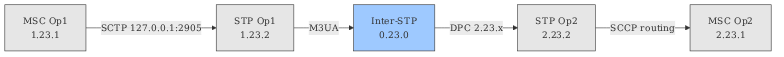
\includegraphics[keepaspectratio]{diagrams/ss7_topology.png}}

Le message suit donc quatre étapes :

\begin{enumerate}
\def\labelenumi{\arabic{enumi}.}
\tightlist
\item
  le \textbf{MSC} envoie le message au \textbf{STP local}
\item
  le STP local transmet le message à l'\textbf{Inter-STP}
\item
  l'Inter-STP sélectionne l'opérateur cible
\item
  le STP distant délivre le message au \textbf{MSC destinataire}
\end{enumerate}

Ce mécanisme reproduit exactement la logique d'interconnexion des
réseaux mobiles.

\begin{center}\rule{0.5\linewidth}{0.5pt}\end{center}

\subsection{Fin de la partie SS7 --- Observabilité et
diagnostic}\label{fin-de-la-partie-ss7-observabilituxe9-et-diagnostic}

Une fois l'infrastructure SS7 en place, l'un des aspects les plus
intéressants du laboratoire est la possibilité d'observer la
signalisation en temps réel.

Dans les réseaux opérateurs, l'accès à la signalisation SS7 est
généralement extrêmement restreint. Les équipements de cœur de réseau
sont isolés et les ingénieurs disposent seulement d'outils internes pour
analyser les flux.

Dans ce laboratoire, la situation est radicalement différente : toute la
signalisation peut être inspectée.

Deux mécanismes principaux permettent cette observation :

\begin{itemize}
\tightlist
\item
  les \textbf{interfaces VTY des composants Osmocom}
\item
  les \textbf{captures réseau avec Wireshark}
\end{itemize}

Les interfaces VTY exposent l'état interne des nœuds SS7. Elles
permettent par exemple de vérifier les associations M3UA actives, la
table de routage ou l'état des routes de signalisation.

Une commande simple permet par exemple de consulter les connexions ASP :

\begin{verbatim}
show cs7 instance 0 asp
\end{verbatim}

Cette commande indique si les associations de signalisation sont
\textbf{actives}, \textbf{inactives} ou \textbf{en attente}.

Une autre commande essentielle est :

\begin{verbatim}
show cs7 instance 0 route
\end{verbatim}

Elle affiche la table de routage SS7 et permet de vérifier si les routes
sont disponibles.

Dans un système sain, les routes dynamiques correspondant aux MSC et aux
BSC apparaissent comme \textbf{available}. Si une route apparaît comme
\textbf{PROHIB}, cela signifie que la signalisation ne peut pas
atteindre ce point code.

Ces informations constituent ce que l'on appelle des \textbf{dumps de
signalisation}. Elles permettent de comprendre précisément comment le
réseau prend ses décisions de routage.

\begin{center}\rule{0.5\linewidth}{0.5pt}\end{center}

\subsection{Analyse des flux avec
Wireshark}\label{analyse-des-flux-avec-wireshark}

Le laboratoire permet également de capturer directement les flux de
signalisation transportés sur le réseau Docker.

Les protocoles visibles sont les suivants :

\begin{itemize}
\tightlist
\item
  \textbf{SCTP} --- transport utilisé par SIGTRAN
\item
  \textbf{M3UA} --- encapsulation des messages SS7
\item
  \textbf{SCCP} --- routage de signalisation
\item
  \textbf{MAP} --- gestion des services mobiles
\end{itemize}

Dans Wireshark, quelques filtres simples permettent d'isoler ces
protocoles :

\begin{verbatim}
m3ua
sccp
gsm_map
sctp.srcport == 2908
\end{verbatim}

Ces captures permettent d'observer des procédures fondamentales du
réseau GSM :

\begin{itemize}
\tightlist
\item
  requêtes de localisation d'abonné
\item
  routage des SMS
\item
  messages de gestion de mobilité
\item
  interrogations du HLR
\end{itemize}

Le laboratoire devient ainsi un véritable \textbf{microscope de
signalisation télécom}.

\begin{center}\rule{0.5\linewidth}{0.5pt}\end{center}

\subsection{Conclusion}\label{conclusion}

Les réseaux mobiles modernes reposent sur une architecture complexe dans
laquelle la radio n'est qu'une partie visible de l'infrastructure.

Derrière chaque appel ou chaque SMS se trouve un réseau de signalisation
chargé de coordonner les équipements du cœur de réseau. SS7 a longtemps
constitué l'épine dorsale de cette infrastructure, et bien que les
réseaux évoluent vers des architectures IP plus récentes, les principes
fondamentaux de la signalisation restent similaires.

Le projet \textbf{osmo\_egprs} propose une approche différente de
l'apprentissage des télécommunications : au lieu d'étudier les
protocoles de manière abstraite, il permet de \textbf{reconstruire un
réseau complet}, puis d'observer son fonctionnement interne.

Grâce à la conteneurisation et à l'automatisation de la configuration,
il devient possible de déployer en quelques minutes un environnement qui
reproduit :

\begin{itemize}
\tightlist
\item
  plusieurs réseaux mobiles indépendants
\item
  un backbone de signalisation SS7
\item
  des échanges inter-opérateurs
\item
  des services voix et SMS
\end{itemize}

Ce laboratoire transforme ainsi un système habituellement inaccessible
en un environnement expérimental ouvert.

Il permet non seulement de comprendre l'architecture des réseaux
mobiles, mais aussi d'explorer leur fonctionnement réel --- un pas
essentiel pour quiconque souhaite étudier les télécommunications, leur
histoire et leur sécurité.

\subsection{SDR \& Matériel (UHD,
BladeRF)}\label{sdr-matuxe9riel-uhd-bladerf}

\subsubsection{UHD (USRP/Ettus)}\label{uhd-usrpettus}

\begin{itemize}
\item
  \textbf{libuhd-dev, uhd-host} : Drivers et outils pour USRP.
\item
  \textbf{Images firmware} :
\end{itemize}

\begin{Shaded}
\begin{Highlighting}[]
\ExtensionTok{python3}\NormalTok{ /usr/lib/uhd/utils/uhd\_images\_downloader.py}
\end{Highlighting}
\end{Shaded}

\begin{itemize}
\tightlist
\item
  \textbf{Règle udev} pour détection auto :
\end{itemize}

\begin{Shaded}
\begin{Highlighting}[]
\FunctionTok{wget}\NormalTok{ https://raw.githubusercontent.com/EttusResearch/uhd/refs/heads/master/host/utils/uhd{-}usrp.rules }\KeywordTok{\&\&} \FunctionTok{cp}\NormalTok{ uhd{-}usrp.rules /etc/udev/rules.d/}
\end{Highlighting}
\end{Shaded}

\subsubsection{BladeRF (Nuand)}\label{bladerf-nuand}

\begin{itemize}
\tightlist
\item
  \textbf{libbladerf-dev} + build depuis les sources :
\end{itemize}

\begin{Shaded}
\begin{Highlighting}[]
\FunctionTok{git}\NormalTok{ clone https://github.com/nuand/BladeRF /opt/GSM/BladeRF}
\BuiltInTok{cd}\NormalTok{ /opt/GSM/BladeRF }\KeywordTok{\&\&} \FunctionTok{mkdir}\NormalTok{ build }\KeywordTok{\&\&} \BuiltInTok{cd}\NormalTok{ build}
\FunctionTok{cmake}\NormalTok{ .. }\KeywordTok{\&\&} \FunctionTok{make} \AttributeTok{{-}j}\VariableTok{$(}\FunctionTok{nproc}\VariableTok{)} \KeywordTok{\&\&} \FunctionTok{make}\NormalTok{ install }\KeywordTok{\&\&} \ExtensionTok{ldconfig}
\end{Highlighting}
\end{Shaded}

\begin{center}\rule{0.5\linewidth}{0.5pt}\end{center}

\subsection{Librairies Osmocom de
base}\label{librairies-osmocom-de-base}

Ces librairies sont la fondation de toute la stack GSM Osmocom.

\begin{itemize}
\tightlist
\item
  \textbf{libosmocore} : Primitives GSM, timers, gestion protocoles.
\item
  \textbf{libosmo-netif} : Interfaces réseau.
\item
  \textbf{libosmo-abis} : Support interface Abis (BTS ↔ BSC).
\end{itemize}

\textbf{Build de chaque librairie :}

\begin{Shaded}
\begin{Highlighting}[]
\FunctionTok{git}\NormalTok{ clone https://github.com/osmocom/}\OperatorTok{\textless{}}\NormalTok{repo}\OperatorTok{\textgreater{}}
\BuiltInTok{cd} \OperatorTok{\textless{}}\NormalTok{repo}\OperatorTok{\textgreater{}} \KeywordTok{\&\&} \ExtensionTok{autoreconf} \AttributeTok{{-}fi} \KeywordTok{\&\&} \ExtensionTok{./configure} \KeywordTok{\&\&} \FunctionTok{make} \AttributeTok{{-}j}\VariableTok{$(}\FunctionTok{nproc}\VariableTok{)} \KeywordTok{\&\&} \FunctionTok{make}\NormalTok{ install }\KeywordTok{\&\&} \ExtensionTok{ldconfig}
\end{Highlighting}
\end{Shaded}

\emph{(remplacer \texttt{\textless{}repo\textgreater{}} par le nom de la
librairie)}

\begin{center}\rule{0.5\linewidth}{0.5pt}\end{center}

\subsection{Stack cœur GSM/EDGE}\label{stack-cux153ur-gsmedge}

\pandocbounded{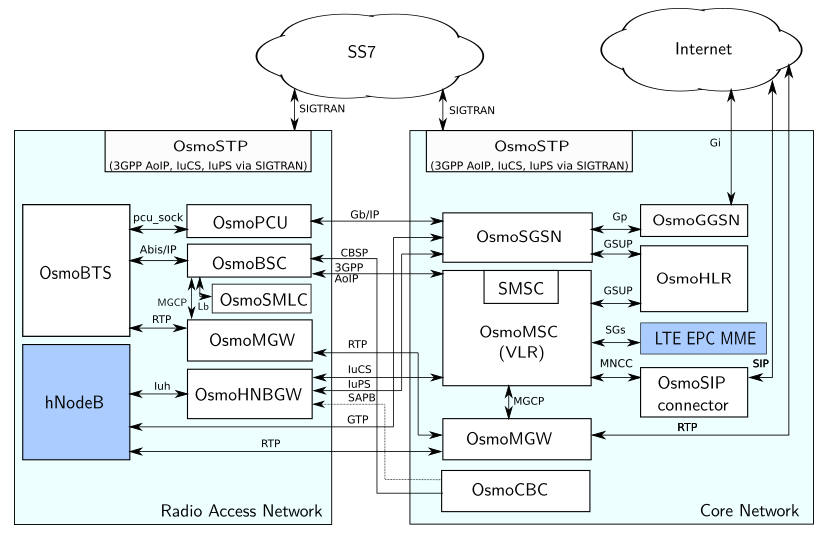
\includegraphics[keepaspectratio]{pictures/osmocom.png}}

\textbf{Osmocom fournit un module séparé pour chaque composant cœur de
réseau :}

\begin{itemize}
\tightlist
\item
  \textbf{osmo-hlr} : Home Location Register (base d'abonnés)
\item
  \textbf{osmo-msc} : Mobile Switching Center (appels, SMS, mobilité)
\item
  \textbf{osmo-bsc} : Base Station Controller (gestion BTS, handover)
\item
  \textbf{osmo-sgsn} : Serving GPRS Support Node (sessions GPRS/EDGE)
\item
  \textbf{osmo-ggsn} : Gateway GPRS Support Node (passerelle IP/data)
\item
  \textbf{osmo-mgw} : Media Gateway (flux voix/data)
\item
  \textbf{osmo-pcu} : Packet Control Unit (gestion trames GPRS/EDGE)
\item
  \textbf{libosmo-sigtran} : SIGTRAN/SS7 over IP
\item
  \textbf{libsmpp34} : Librairie SMPP (SMS)
\item
  \textbf{libgtpnl} : GTP (GPRS Tunneling Protocol pour data mobile)
\end{itemize}

\textbf{Exemple de build générique :}

\begin{Shaded}
\begin{Highlighting}[]
\FunctionTok{git}\NormalTok{ clone https://github.com/osmocom/}\OperatorTok{\textless{}}\NormalTok{module}\OperatorTok{\textgreater{}}
\BuiltInTok{cd} \OperatorTok{\textless{}}\NormalTok{module}\OperatorTok{\textgreater{}} \KeywordTok{\&\&} \ExtensionTok{autoreconf} \AttributeTok{{-}fi} \KeywordTok{\&\&} \ExtensionTok{./configure} \PreprocessorTok{[}\SpecialStringTok{OPTIONS}\PreprocessorTok{]} \KeywordTok{\&\&} \FunctionTok{make} \AttributeTok{{-}j}\VariableTok{$(}\FunctionTok{nproc}\VariableTok{)} \KeywordTok{\&\&} \FunctionTok{make}\NormalTok{ install }\KeywordTok{\&\&} \ExtensionTok{ldconfig}
\end{Highlighting}
\end{Shaded}

\begin{itemize}
\tightlist
\item
  Les options comme \texttt{-\/-enable-gtp-linux},
  \texttt{-\/-enable-iu}, \texttt{-\/-enable-smpp}, etc, dépendent du
  module.
\end{itemize}

\begin{center}\rule{0.5\linewidth}{0.5pt}\end{center}

\subsection{Couches radio (TRX/BTS)}\label{couches-radio-trxbts}

\begin{itemize}
\item
  \textbf{osmo-trx} : Transceiver SDR (modulation, A5/x, couche radio
  PHY)
\item
  \textbf{osmo-bts} : Interface logicielle pour le TRX (logiciel BTS)

  \begin{itemize}
  \tightlist
  \item
    Option : \texttt{-\/-enable-trx} pour activer le mode SDR.
  \end{itemize}
\end{itemize}

\textbf{Build typique :}

\begin{Shaded}
\begin{Highlighting}[]
\FunctionTok{git}\NormalTok{ clone https://github.com/osmocom/osmo{-}trx}
\BuiltInTok{cd}\NormalTok{ osmo{-}trx }\KeywordTok{\&\&} \ExtensionTok{autoreconf} \AttributeTok{{-}fi} \KeywordTok{\&\&} \ExtensionTok{./configure} \AttributeTok{{-}{-}with{-}uhd} \KeywordTok{\&\&} \FunctionTok{make} \AttributeTok{{-}j}\VariableTok{$(}\FunctionTok{nproc}\VariableTok{)} \KeywordTok{\&\&} \FunctionTok{make}\NormalTok{ install }\KeywordTok{\&\&} \ExtensionTok{ldconfig}

\FunctionTok{git}\NormalTok{ clone https://github.com/osmocom/osmo{-}bts}
\BuiltInTok{cd}\NormalTok{ osmo{-}bts }\KeywordTok{\&\&} \ExtensionTok{autoreconf} \AttributeTok{{-}fi} \KeywordTok{\&\&} \ExtensionTok{./configure} \AttributeTok{{-}{-}enable{-}trx} \KeywordTok{\&\&} \FunctionTok{make} \AttributeTok{{-}j}\VariableTok{$(}\FunctionTok{nproc}\VariableTok{)} \KeywordTok{\&\&} \FunctionTok{make}\NormalTok{ install }\KeywordTok{\&\&} \ExtensionTok{ldconfig}
\end{Highlighting}
\end{Shaded}

\begin{center}\rule{0.5\linewidth}{0.5pt}\end{center}

\subsection{Services \& Outils
additionnels}\label{services-outils-additionnels}

\begin{itemize}
\tightlist
\item
  \textbf{osmo-sip-connector} : passerelle GSM ↔ VoIP SIP (pour appels
  IP)
\item
  \textbf{Outils SIM} : \texttt{pcsc-tools}, \texttt{pcscd},
  \texttt{libpcsclite-dev}
\item
  \textbf{iptables}, \textbf{tmux}, \textbf{nano}, \textbf{python3-pip}
  : utilitaires système
\item
  \textbf{python3-requests} : scripts API/réseau
\end{itemize}

\textbf{Exemple d'installation :}

\begin{Shaded}
\begin{Highlighting}[]
\ExtensionTok{apt}\NormalTok{ install }\AttributeTok{{-}y}\NormalTok{ iptables tmux nano python3{-}pip python3{-}requests}
\ExtensionTok{pip3}\NormalTok{ install requests}
\end{Highlighting}
\end{Shaded}

\begin{center}\rule{0.5\linewidth}{0.5pt}\end{center}

\subsection{Script modulaire (bash)}\label{script-modulaire-bash}

\begin{Shaded}
\begin{Highlighting}[]
\CommentTok{\#!/bin/bash}
\CommentTok{\# Installeur modulaire EGPRS/Osmocom}
\CommentTok{\# Construit une stack GSM/EDGE complète avec SDR : USRP, BladeRF, Osmocom core et toutes dépendances.}
\CommentTok{\# Auteur : Bastien / bbaranoff (software{-}defined{-}radio.com)}
\CommentTok{\# Testé sur Ubuntu 22.04+}

\BuiltInTok{set} \AttributeTok{{-}e}
\VariableTok{N}\OperatorTok{=}\VariableTok{$(}\FunctionTok{nproc}\VariableTok{)} \KeywordTok{||} \VariableTok{N}\OperatorTok{=}\NormalTok{2}
\VariableTok{ROOT}\OperatorTok{=}\NormalTok{/opt/GSM}

\CommentTok{\# {-}{-}{-}{-}{-}{-}{-}{-}{-}{-}{-}{-}{-}{-}{-}{-}{-}{-}{-}{-}{-}{-}{-}{-}{-}{-}{-}{-}{-}{-}{-}{-}{-}{-}{-}{-}{-}{-}{-}{-}}
\CommentTok{\#  Dépendances système}
\CommentTok{\# {-}{-}{-}{-}{-}{-}{-}{-}{-}{-}{-}{-}{-}{-}{-}{-}{-}{-}{-}{-}{-}{-}{-}{-}{-}{-}{-}{-}{-}{-}{-}{-}{-}{-}{-}{-}{-}{-}{-}{-}}
\FunctionTok{install\_deps()} \KeywordTok{\{}
    \BuiltInTok{echo} \StringTok{"==\textgreater{} Installation des paquets système et dépendances de build..."}
    \ExtensionTok{apt}\NormalTok{ update}
    \ExtensionTok{apt}\NormalTok{ install }\AttributeTok{{-}y} \DataTypeTok{\textbackslash{}}
\NormalTok{        gcc g++ make cmake autoconf automake libtool pkg{-}config }\DataTypeTok{\textbackslash{}}
\NormalTok{        libedit{-}dev libfftw3{-}dev libusb{-}1.0{-}0{-}dev liburing{-}dev }\DataTypeTok{\textbackslash{}}
\NormalTok{        nano git wget curl tmux doxygen ethtool }\DataTypeTok{\textbackslash{}}
\NormalTok{        python3 python3{-}dev python3{-}pip python3{-}six python3{-}mako python3{-}lxml python3{-}numpy python3{-}pybind11 python3{-}requests python3{-}scipy python3{-}setuptools python3{-}ruamel.yaml }\DataTypeTok{\textbackslash{}}
\NormalTok{        libpcsclite{-}dev pcsc{-}tools pcscd cpufrequtils libsctp{-}dev libconfig++{-}dev libconfig{-}dev libmbedtls{-}dev }\DataTypeTok{\textbackslash{}}
\NormalTok{        libtalloc{-}dev libgnutls28{-}dev libmnl{-}dev libortp{-}dev libdbd{-}sqlite3 iproute2 iputils{-}ping }\DataTypeTok{\textbackslash{}}
\NormalTok{        libsqlite3{-}dev libdbi{-}dev libc{-}ares{-}dev libsofia{-}sip{-}ua{-}glib{-}dev telnet }\DataTypeTok{\textbackslash{}}
\NormalTok{        systemd systemd{-}sysv dbus dbus{-}user{-}session ccache libboost{-}all{-}dev libncurses5 libncurses5{-}dev }\DataTypeTok{\textbackslash{}}
\NormalTok{        libusb{-}1.0{-}0 libusb{-}dev iptables udev}
\KeywordTok{\}}

\CommentTok{\# {-}{-}{-}{-}{-}{-}{-}{-}{-}{-}{-}{-}{-}{-}{-}{-}{-}{-}{-}{-}{-}{-}{-}{-}{-}{-}{-}{-}{-}{-}{-}{-}{-}{-}{-}{-}{-}{-}{-}{-}}
\CommentTok{\#  Drivers SDR \& Firmware}
\CommentTok{\# {-}{-}{-}{-}{-}{-}{-}{-}{-}{-}{-}{-}{-}{-}{-}{-}{-}{-}{-}{-}{-}{-}{-}{-}{-}{-}{-}{-}{-}{-}{-}{-}{-}{-}{-}{-}{-}{-}{-}{-}}

\FunctionTok{install\_uhd()} \KeywordTok{\{}
    \BuiltInTok{echo} \StringTok{"==\textgreater{} Installation UHD/USRP et téléchargement images firmware..."}
    \ExtensionTok{apt}\NormalTok{ install }\AttributeTok{{-}y}\NormalTok{ libuhd{-}dev uhd{-}host}
    \ExtensionTok{python3}\NormalTok{ /usr/lib/uhd/utils/uhd\_images\_downloader.py}
    \CommentTok{\# Règles udev Ettus USRP}
    \FunctionTok{wget} \AttributeTok{{-}O}\NormalTok{ /etc/udev/rules.d/uhd{-}usrp.rules https://raw.githubusercontent.com/EttusResearch/uhd/refs/heads/master/host/utils/uhd{-}usrp.rules}
    \BuiltInTok{echo} \StringTok{"export UHD\_MODULE\_PATH=/usr/lib/uhd/modules"} \OperatorTok{\textgreater{}\textgreater{}}\NormalTok{ /root/.bashrc}
\KeywordTok{\}}

\FunctionTok{install\_bladerf()} \KeywordTok{\{}
    \BuiltInTok{echo} \StringTok{"==\textgreater{} Installation BladeRF et build depuis sources..."}
    \ExtensionTok{apt}\NormalTok{ install }\AttributeTok{{-}y}\NormalTok{ libbladerf{-}dev}
    \FunctionTok{git}\NormalTok{ clone https://github.com/nuand/BladeRF }\VariableTok{$ROOT}\NormalTok{/BladeRF }\KeywordTok{||} \FunctionTok{true}
    \BuiltInTok{cd} \VariableTok{$ROOT}\NormalTok{/BladeRF}
    \FunctionTok{mkdir} \AttributeTok{{-}p}\NormalTok{ build }\KeywordTok{\&\&} \BuiltInTok{cd}\NormalTok{ build}
    \FunctionTok{cmake}\NormalTok{ .. }\KeywordTok{\&\&} \FunctionTok{make} \AttributeTok{{-}j}\VariableTok{$N} \KeywordTok{\&\&} \FunctionTok{make}\NormalTok{ install }\KeywordTok{\&\&} \ExtensionTok{ldconfig}
\KeywordTok{\}}

\CommentTok{\# {-}{-}{-}{-}{-}{-}{-}{-}{-}{-}{-}{-}{-}{-}{-}{-}{-}{-}{-}{-}{-}{-}{-}{-}{-}{-}{-}{-}{-}{-}{-}{-}{-}{-}{-}{-}{-}{-}{-}{-}}
\CommentTok{\# Librairies Osmocom de base}
\CommentTok{\# {-}{-}{-}{-}{-}{-}{-}{-}{-}{-}{-}{-}{-}{-}{-}{-}{-}{-}{-}{-}{-}{-}{-}{-}{-}{-}{-}{-}{-}{-}{-}{-}{-}{-}{-}{-}{-}{-}{-}{-}}
\FunctionTok{build\_osmo\_lib()} \KeywordTok{\{}
    \BuiltInTok{echo} \StringTok{"==\textgreater{} Build des librairies Osmocom : libosmocore, libosmo{-}netif, libosmo{-}abis"}
    \ControlFlowTok{for}\NormalTok{ repo }\KeywordTok{in}\NormalTok{ libosmocore libosmo{-}netif libosmo{-}abis}\KeywordTok{;} \ControlFlowTok{do}
        \FunctionTok{git}\NormalTok{ clone https://github.com/osmocom/}\VariableTok{$repo} \VariableTok{$ROOT}\NormalTok{/}\VariableTok{$repo} \KeywordTok{||} \FunctionTok{true}
        \BuiltInTok{cd} \VariableTok{$ROOT}\NormalTok{/}\VariableTok{$repo}
        \ExtensionTok{autoreconf} \AttributeTok{{-}fi}
        \ExtensionTok{./configure}
        \FunctionTok{make} \AttributeTok{{-}j}\VariableTok{$N}
        \FunctionTok{make}\NormalTok{ install}
        \ExtensionTok{ldconfig}
    \ControlFlowTok{done}
\KeywordTok{\}}

\CommentTok{\# {-}{-}{-}{-}{-}{-}{-}{-}{-}{-}{-}{-}{-}{-}{-}{-}{-}{-}{-}{-}{-}{-}{-}{-}{-}{-}{-}{-}{-}{-}{-}{-}{-}{-}{-}{-}{-}{-}{-}{-}}
\CommentTok{\# Réseau cœur, radio, EDGE}
\CommentTok{\# {-}{-}{-}{-}{-}{-}{-}{-}{-}{-}{-}{-}{-}{-}{-}{-}{-}{-}{-}{-}{-}{-}{-}{-}{-}{-}{-}{-}{-}{-}{-}{-}{-}{-}{-}{-}{-}{-}{-}{-}}
\FunctionTok{build\_osmo\_core()} \KeywordTok{\{}
    \BuiltInTok{echo} \StringTok{"==\textgreater{} Build Osmocom réseau, radio et modules GPRS..."}
    
    \CommentTok{\# HLR (DB abonnés)}
    \FunctionTok{git}\NormalTok{ clone https://github.com/osmocom/osmo{-}hlr }\VariableTok{$ROOT}\NormalTok{/osmo{-}hlr }\KeywordTok{||} \FunctionTok{true}
    \BuiltInTok{cd} \VariableTok{$ROOT}\NormalTok{/osmo{-}hlr }\KeywordTok{\&\&} \ExtensionTok{autoreconf} \AttributeTok{{-}fi} \KeywordTok{\&\&} \ExtensionTok{./configure} \KeywordTok{\&\&} \FunctionTok{make} \AttributeTok{{-}j}\VariableTok{$N} \KeywordTok{\&\&} \FunctionTok{make}\NormalTok{ install }\KeywordTok{\&\&} \ExtensionTok{ldconfig}

    \CommentTok{\# Media Gateway}
    \FunctionTok{git}\NormalTok{ clone https://github.com/osmocom/osmo{-}mgw }\VariableTok{$ROOT}\NormalTok{/osmo{-}mgw }\KeywordTok{||} \FunctionTok{true}
    \BuiltInTok{cd} \VariableTok{$ROOT}\NormalTok{/osmo{-}mgw }\KeywordTok{\&\&} \ExtensionTok{autoreconf} \AttributeTok{{-}fi} \KeywordTok{\&\&} \ExtensionTok{./configure} \KeywordTok{\&\&} \FunctionTok{make} \AttributeTok{{-}j}\VariableTok{$N} \KeywordTok{\&\&} \FunctionTok{make}\NormalTok{ install }\KeywordTok{\&\&} \ExtensionTok{ldconfig}

    \CommentTok{\# SIGTRAN (SS7 sur IP)}
    \FunctionTok{git}\NormalTok{ clone https://gitea.osmocom.org/osmocom/libosmo{-}sigtran }\VariableTok{$ROOT}\NormalTok{/libosmo{-}sigtran }\KeywordTok{||} \FunctionTok{true}
    \BuiltInTok{cd} \VariableTok{$ROOT}\NormalTok{/libosmo{-}sigtran }\KeywordTok{\&\&} \ExtensionTok{autoreconf} \AttributeTok{{-}fi} \KeywordTok{\&\&} \ExtensionTok{./configure} \KeywordTok{\&\&} \FunctionTok{make} \AttributeTok{{-}j}\VariableTok{$N} \KeywordTok{\&\&} \FunctionTok{make}\NormalTok{ install }\KeywordTok{\&\&} \ExtensionTok{ldconfig}

    \CommentTok{\# libsmpp34 (SMS)}
    \FunctionTok{git}\NormalTok{ clone https://github.com/osmocom/libsmpp34 }\VariableTok{$ROOT}\NormalTok{/libsmpp34 }\KeywordTok{||} \FunctionTok{true}
    \BuiltInTok{cd} \VariableTok{$ROOT}\NormalTok{/libsmpp34 }\KeywordTok{\&\&} \ExtensionTok{autoreconf} \AttributeTok{{-}fi} \KeywordTok{\&\&} \ExtensionTok{./configure} \KeywordTok{\&\&} \FunctionTok{make} \AttributeTok{{-}j}\VariableTok{$N} \KeywordTok{\&\&} \FunctionTok{make}\NormalTok{ install }\KeywordTok{\&\&} \ExtensionTok{ldconfig}

    \CommentTok{\# libgtpnl (tunnels GTP)}
    \FunctionTok{git}\NormalTok{ clone https://github.com/osmocom/libgtpnl }\VariableTok{$ROOT}\NormalTok{/libgtpnl }\KeywordTok{||} \FunctionTok{true}
    \BuiltInTok{cd} \VariableTok{$ROOT}\NormalTok{/libgtpnl }\KeywordTok{\&\&} \ExtensionTok{autoreconf} \AttributeTok{{-}fi} \KeywordTok{\&\&} \ExtensionTok{./configure} \AttributeTok{{-}{-}enable{-}gtp{-}linux} \KeywordTok{\&\&} \FunctionTok{make} \AttributeTok{{-}j}\VariableTok{$N} \KeywordTok{\&\&} \FunctionTok{make}\NormalTok{ install }\KeywordTok{\&\&} \ExtensionTok{ldconfig}

    \CommentTok{\# Éléments cœur (ordre : GGSN, SGSN, MSC, BSC, PCU)}
    \FunctionTok{git}\NormalTok{ clone https://github.com/osmocom/osmo{-}ggsn }\VariableTok{$ROOT}\NormalTok{/osmo{-}ggsn }\KeywordTok{||} \FunctionTok{true}
    \BuiltInTok{cd} \VariableTok{$ROOT}\NormalTok{/osmo{-}ggsn }\KeywordTok{\&\&} \ExtensionTok{autoreconf} \AttributeTok{{-}fi} \KeywordTok{\&\&} \ExtensionTok{./configure} \AttributeTok{{-}{-}enable{-}gtp{-}linux} \KeywordTok{\&\&} \FunctionTok{make} \AttributeTok{{-}j}\VariableTok{$N} \KeywordTok{\&\&} \FunctionTok{make}\NormalTok{ install }\KeywordTok{\&\&} \ExtensionTok{ldconfig}

    \FunctionTok{git}\NormalTok{ clone https://github.com/osmocom/osmo{-}sgsn }\VariableTok{$ROOT}\NormalTok{/osmo{-}sgsn }\KeywordTok{||} \FunctionTok{true}
    \BuiltInTok{cd} \VariableTok{$ROOT}\NormalTok{/osmo{-}sgsn }\KeywordTok{\&\&} \ExtensionTok{autoreconf} \AttributeTok{{-}fi} \KeywordTok{\&\&} \ExtensionTok{./configure} \AttributeTok{{-}{-}enable{-}iu} \KeywordTok{\&\&} \FunctionTok{make} \AttributeTok{{-}j}\VariableTok{$N} \KeywordTok{\&\&} \FunctionTok{make}\NormalTok{ install }\KeywordTok{\&\&} \ExtensionTok{ldconfig}

    \FunctionTok{git}\NormalTok{ clone https://github.com/osmocom/osmo{-}msc }\VariableTok{$ROOT}\NormalTok{/osmo{-}msc }\KeywordTok{||} \FunctionTok{true}
    \BuiltInTok{cd} \VariableTok{$ROOT}\NormalTok{/osmo{-}msc }\KeywordTok{\&\&} \ExtensionTok{autoreconf} \AttributeTok{{-}fi} \KeywordTok{\&\&} \ExtensionTok{./configure} \AttributeTok{{-}{-}enable{-}smpp} \AttributeTok{{-}{-}enable{-}iu} \KeywordTok{\&\&} \FunctionTok{make} \AttributeTok{{-}j}\VariableTok{$N} \KeywordTok{\&\&} \FunctionTok{make}\NormalTok{ install }\KeywordTok{\&\&} \ExtensionTok{ldconfig}

    \FunctionTok{git}\NormalTok{ clone https://github.com/osmocom/osmo{-}bsc }\VariableTok{$ROOT}\NormalTok{/osmo{-}bsc }\KeywordTok{||} \FunctionTok{true}
    \BuiltInTok{cd} \VariableTok{$ROOT}\NormalTok{/osmo{-}bsc }\KeywordTok{\&\&} \ExtensionTok{autoreconf} \AttributeTok{{-}fi} \KeywordTok{\&\&} \ExtensionTok{./configure} \AttributeTok{{-}{-}enable{-}iu} \KeywordTok{\&\&} \FunctionTok{make} \AttributeTok{{-}j}\VariableTok{$N} \KeywordTok{\&\&} \FunctionTok{make}\NormalTok{ install }\KeywordTok{\&\&} \ExtensionTok{ldconfig}

    \FunctionTok{git}\NormalTok{ clone https://github.com/osmocom/osmo{-}pcu }\VariableTok{$ROOT}\NormalTok{/osmo{-}pcu }\KeywordTok{||} \FunctionTok{true}
    \BuiltInTok{cd} \VariableTok{$ROOT}\NormalTok{/osmo{-}pcu }\KeywordTok{\&\&} \ExtensionTok{autoreconf} \AttributeTok{{-}fi} \KeywordTok{\&\&} \ExtensionTok{./configure} \KeywordTok{\&\&} \FunctionTok{make} \AttributeTok{{-}j}\VariableTok{$N} \KeywordTok{\&\&} \FunctionTok{make}\NormalTok{ install }\KeywordTok{\&\&} \ExtensionTok{ldconfig}

    \CommentTok{\# Couches radio : TRX, BTS}
    \FunctionTok{git}\NormalTok{ clone https://github.com/osmocom/osmo{-}trx }\VariableTok{$ROOT}\NormalTok{/osmo{-}trx }\KeywordTok{||} \FunctionTok{true}
    \BuiltInTok{cd} \VariableTok{$ROOT}\NormalTok{/osmo{-}trx }\KeywordTok{\&\&} \ExtensionTok{autoreconf} \AttributeTok{{-}fi} \KeywordTok{\&\&} \ExtensionTok{./configure} \AttributeTok{{-}{-}with{-}uhd} \KeywordTok{\&\&} \FunctionTok{make} \AttributeTok{{-}j}\VariableTok{$N} \KeywordTok{\&\&} \FunctionTok{make}\NormalTok{ install }\KeywordTok{\&\&} \ExtensionTok{ldconfig}

    \FunctionTok{git}\NormalTok{ clone https://github.com/osmocom/osmo{-}bts }\VariableTok{$ROOT}\NormalTok{/osmo{-}bts }\KeywordTok{||} \FunctionTok{true}
    \BuiltInTok{cd} \VariableTok{$ROOT}\NormalTok{/osmo{-}bts }\KeywordTok{\&\&} \ExtensionTok{autoreconf} \AttributeTok{{-}fi} \KeywordTok{\&\&} \ExtensionTok{./configure} \AttributeTok{{-}{-}enable{-}trx} \KeywordTok{\&\&} \FunctionTok{make} \AttributeTok{{-}j}\VariableTok{$N} \KeywordTok{\&\&} \FunctionTok{make}\NormalTok{ install }\KeywordTok{\&\&} \ExtensionTok{ldconfig}

    \CommentTok{\# SIP connector (SIP/VoIP)}
    \FunctionTok{git}\NormalTok{ clone https://github.com/osmocom/osmo{-}sip{-}connector }\VariableTok{$ROOT}\NormalTok{/osmo{-}sip{-}connector }\KeywordTok{||} \FunctionTok{true}
    \BuiltInTok{cd} \VariableTok{$ROOT}\NormalTok{/osmo{-}sip{-}connector }\KeywordTok{\&\&} \ExtensionTok{autoreconf} \AttributeTok{{-}fi} \KeywordTok{\&\&} \ExtensionTok{./configure} \KeywordTok{\&\&} \FunctionTok{make} \AttributeTok{{-}j}\VariableTok{$N} \KeywordTok{\&\&} \FunctionTok{make}\NormalTok{ install }\KeywordTok{\&\&} \ExtensionTok{ldconfig}
\KeywordTok{\}}

\CommentTok{\# {-}{-}{-}{-}{-}{-}{-}{-}{-}{-}{-}{-}{-}{-}{-}{-}{-}{-}{-}{-}{-}{-}{-}{-}{-}{-}{-}{-}{-}{-}{-}{-}{-}{-}{-}{-}{-}{-}{-}{-}}
\CommentTok{\# Python \& utilitaires système}
\CommentTok{\# {-}{-}{-}{-}{-}{-}{-}{-}{-}{-}{-}{-}{-}{-}{-}{-}{-}{-}{-}{-}{-}{-}{-}{-}{-}{-}{-}{-}{-}{-}{-}{-}{-}{-}{-}{-}{-}{-}{-}{-}}
\FunctionTok{install\_python\_utils()} \KeywordTok{\{}
    \BuiltInTok{echo} \StringTok{"==\textgreater{} Installation dépendances pip et update images UHD..."}
    \ExtensionTok{pip3}\NormalTok{ install requests}
    \CommentTok{\# (Re)télécharge images firmware UHD si besoin}
    \ExtensionTok{python3}\NormalTok{ /usr/lib/uhd/utils/uhd\_images\_downloader.py }\KeywordTok{||} \FunctionTok{true}
\KeywordTok{\}}

\CommentTok{\# {-}{-}{-}{-}{-}{-}{-}{-}{-}{-}{-}{-}{-}{-}{-}{-}{-}{-}{-}{-}{-}{-}{-}{-}{-}{-}{-}{-}{-}{-}{-}{-}{-}{-}{-}{-}{-}{-}{-}{-}}
\CommentTok{\# Séquence principale}
\CommentTok{\# {-}{-}{-}{-}{-}{-}{-}{-}{-}{-}{-}{-}{-}{-}{-}{-}{-}{-}{-}{-}{-}{-}{-}{-}{-}{-}{-}{-}{-}{-}{-}{-}{-}{-}{-}{-}{-}{-}{-}{-}}
\FunctionTok{main()} \KeywordTok{\{}
    \ExtensionTok{install\_deps}
    \ExtensionTok{install\_uhd}
    \ExtensionTok{install\_bladerf}
    \ExtensionTok{build\_osmo\_lib}
    \ExtensionTok{build\_osmo\_core}
    \ExtensionTok{install\_python\_utils}
    \BuiltInTok{echo} \StringTok{"==\textgreater{} Tous les modules sont installés. Vous pouvez passer à la configuration et aux scripts de run."}
\KeywordTok{\}}

\ExtensionTok{main} \StringTok{"}\VariableTok{$@}\StringTok{"}
\end{Highlighting}
\end{Shaded}

\begin{center}\rule{0.5\linewidth}{0.5pt}\end{center}

\subsection{Résumé \& Bonnes
pratiques}\label{ruxe9sumuxe9-bonnes-pratiques}

\begin{itemize}
\tightlist
\item
  \textbf{Chaque module} est un bloc indépendant, à construire dans
  l'ordre (libs → cœur → radio → services)
\item
  Pour EGPRS, l'ordre \textbf{BTS/TRX/PCU/SGSN/GGSN} est crucial (le
  flux data traverse chaque élément)
\item
  \textbf{Séparation des modules} = maintenance et debug facilités
\item
  Toujours vérifier les dépendances système/matériel (drivers USRP,
  firmware BladeRF, règles udev\ldots)
\end{itemize}

\subsection{Installation d'une BTS OsmocomBB
Calypso}\label{installation-dune-bts-osmocombb-calypso}

\subsection{Matériel requis}\label{matuxe9riel-requis}

\begin{itemize}
\tightlist
\item
  1-2x Motorola C1xx (C115, C118, C123\ldots{} chipset Calypso)
\item
  2x Câbles USB-série jack 2.5\,mm (PL2303/FTDI)
\item
  Ubuntu 24.04 x86\_64 (VM ou natif)
\item
  Accès root
\end{itemize}

\begin{center}\rule{0.5\linewidth}{0.5pt}\end{center}

\subsection{Dépendances système}\label{duxe9pendances-systuxe8me-1}

\begin{Shaded}
\begin{Highlighting}[]
\FunctionTok{sudo}\NormalTok{ apt update}
\FunctionTok{sudo}\NormalTok{ apt install }\AttributeTok{{-}y} \DataTypeTok{\textbackslash{}}
\NormalTok{  build{-}essential git cmake pkg{-}config autoconf automake libtool shtool }\DataTypeTok{\textbackslash{}}
\NormalTok{  bison flex libtalloc{-}dev libpcsclite{-}dev zlib1g{-}dev libmpfr{-}dev libmpc{-}dev }\DataTypeTok{\textbackslash{}}
\NormalTok{  libgmp{-}dev libncurses5{-}dev libncursesw5{-}dev libsofia{-}sip{-}ua{-}dev libxml2{-}dev }\DataTypeTok{\textbackslash{}}
\NormalTok{  libfftw3{-}dev libgnutls28{-}dev libssl{-}dev python3 python3{-}pip }\DataTypeTok{\textbackslash{}}
\NormalTok{  alsa{-}oss lemon libtinfo{-}dev}
\end{Highlighting}
\end{Shaded}

\begin{quote}
\textbf{Note}\,: Ubuntu 24.04 a GCC\,13+ par défaut, mais il faut
parfois cross-compiler avec GCC 4.9 pour le firmware Calypso. S'il
existe des binaires arm-elf précompilés pour Ubuntu 22.04, ils
fonctionnent aussi sous 24.04. Pour l'ARM toolchain, voir plus bas
(utilise de préférence un container/VM si souci d'incompatibilité).
\end{quote}

\begin{center}\rule{0.5\linewidth}{0.5pt}\end{center}

\subsection{Installer la toolchain ARM-elf (cross-compiler
Calypso)}\label{installer-la-toolchain-arm-elf-cross-compiler-calypso}

\subsubsection{Option A\,: Téléchargement direct (prêt à
l'emploi)}\label{option-a-tuxe9luxe9chargement-direct-pruxeat-uxe0-lemploi}

\begin{Shaded}
\begin{Highlighting}[]
\CommentTok{\# Depuis Osmocom (préconisé : ne pas compiler vous{-}même sous Ubuntu récent)}
\BuiltInTok{cd}\NormalTok{ /opt}
\FunctionTok{sudo}\NormalTok{ wget https://downloads.osmocom.org/binaries/toolchain/arm{-}2021.03.tar.bz2}
\FunctionTok{sudo}\NormalTok{ tar }\AttributeTok{{-}xjf}\NormalTok{ arm{-}2021.03.tar.bz2}
\BuiltInTok{export} \VariableTok{PATH}\OperatorTok{=}\VariableTok{$PATH}\NormalTok{:/opt/arm{-}2021.03/bin}
\end{Highlighting}
\end{Shaded}

\begin{quote}
\textbf{Ajoute l'export PATH à ton .bashrc pour persistance}
\end{quote}

\subsubsection{Option B\,: Compilation
manuelle}\label{option-b-compilation-manuelle}

\begin{quote}
(non recommandé sur Ubuntu 24.04, c'est lent et casse souvent, préfère
la méthode ci-dessus)
\end{quote}

\begin{center}\rule{0.5\linewidth}{0.5pt}\end{center}

\subsection{Compiler et installer
OsmocomBB}\label{compiler-et-installer-osmocombb}

\begin{Shaded}
\begin{Highlighting}[]
\CommentTok{\# Cloner les sources}
\FunctionTok{git}\NormalTok{ clone https://github.com/osmocom/osmocom{-}bb.git}
\BuiltInTok{cd}\NormalTok{ osmocom{-}bb}

\CommentTok{\# Préparer le build}
\BuiltInTok{cd}\NormalTok{ src}
\ExtensionTok{autoreconf} \AttributeTok{{-}i}

\CommentTok{\# Compiler le firmware (spécifie la toolchain si besoin)}
\BuiltInTok{export} \VariableTok{PATH}\OperatorTok{=}\VariableTok{$PATH}\NormalTok{:/opt/arm{-}2021.03/bin}
\ExtensionTok{./configure}
\FunctionTok{make} \AttributeTok{{-}j}\VariableTok{$(}\FunctionTok{nproc}\VariableTok{)}
\FunctionTok{sudo}\NormalTok{ make install}
\FunctionTok{sudo}\NormalTok{ ldconfig}
\end{Highlighting}
\end{Shaded}

\begin{center}\rule{0.5\linewidth}{0.5pt}\end{center}

\subsection{Flasher le firmware sur les
téléphones}\label{flasher-le-firmware-sur-les-tuxe9luxe9phones}

\textbf{Connecte les deux téléphones via USB-PL2303, batterie retirée.}

\begin{Shaded}
\begin{Highlighting}[]
\BuiltInTok{cd}\NormalTok{ src/host/osmocon}
\FunctionTok{sudo}\NormalTok{ ./osmocon }\AttributeTok{{-}m}\NormalTok{ c123xor }\AttributeTok{{-}p}\NormalTok{ /dev/ttyUSB0 }\AttributeTok{{-}c}\NormalTok{ ../../target/firmware/board/compal\_e88/rssi.highram.bin}
\CommentTok{\# (Shell \#1 : RSSI scan, contrôle{-}C pour arrêter)}
\end{Highlighting}
\end{Shaded}

\textbf{Trouve un ARFCN actif (fort signal GSM, ex.~: 900/1800 MHz).}

\begin{Shaded}
\begin{Highlighting}[]
\CommentTok{\# Pour charger le firmware TRX (BTS)}
\FunctionTok{sudo}\NormalTok{ ./osmocon }\AttributeTok{{-}m}\NormalTok{ c123xor }\AttributeTok{{-}p}\NormalTok{ /dev/ttyUSB0 }\AttributeTok{{-}s}\NormalTok{ /tmp/osmocom\_l2 }\DataTypeTok{\textbackslash{}}
  \AttributeTok{{-}c}\NormalTok{ ../../target/firmware/board/compal\_e88/trx.highram.bin }\AttributeTok{{-}r}\NormalTok{ 99}
\FunctionTok{sudo}\NormalTok{ ./osmocon }\AttributeTok{{-}m}\NormalTok{ c123xor }\AttributeTok{{-}p}\NormalTok{ /dev/ttyUSB1 }\AttributeTok{{-}s}\NormalTok{ /tmp/osmocom\_l2.2 }\DataTypeTok{\textbackslash{}}
  \AttributeTok{{-}c}\NormalTok{ ../../target/firmware/board/compal\_e88/trx.highram.bin }\AttributeTok{{-}r}\NormalTok{ 99}
\end{Highlighting}
\end{Shaded}

\begin{center}\rule{0.5\linewidth}{0.5pt}\end{center}

\subsection{Lancer le transceiver et la stack
BTS}\label{lancer-le-transceiver-et-la-stack-bts}

Dans d'autres shells\,:

\begin{Shaded}
\begin{Highlighting}[]
\CommentTok{\# Shell \#3 : transceiver Calypso (remplace ARFCN trouvé)}
\BuiltInTok{cd}\NormalTok{ src/host/layer23/src/transceiver/}
\FunctionTok{sudo}\NormalTok{ ./transceiver }\AttributeTok{{-}a} \PreprocessorTok{[}\SpecialStringTok{ARFCN}\PreprocessorTok{]} \AttributeTok{{-}2} \AttributeTok{{-}r}\NormalTok{ 99}

\CommentTok{\# Shell \#4 : osmo{-}nitb (NITB = core minimal)}
\ExtensionTok{osmo{-}nitb} \AttributeTok{{-}c}\NormalTok{ \textasciitilde{}/.osmocom/open{-}bsc.cfg }\AttributeTok{{-}l}\NormalTok{ \textasciitilde{}/.osmocom/hlr.sqlite3 }\AttributeTok{{-}P} \AttributeTok{{-}m} \AttributeTok{{-}C} \AttributeTok{{-}{-}debug}\OperatorTok{=}\NormalTok{DRLL:DCC:DMM:DRR:DRSL:DNM}

\CommentTok{\# Shell \#5 : osmobts{-}trx}
\ExtensionTok{osmobts{-}trx} \AttributeTok{{-}c}\NormalTok{ \textasciitilde{}/.osmocom/osmo{-}bts.cfg }\AttributeTok{{-}r}\NormalTok{ 99}
\end{Highlighting}
\end{Shaded}

\begin{center}\rule{0.5\linewidth}{0.5pt}\end{center}

\subsection{(Optionnel) Installer Asterisk + LCR pour appels
SIP}\label{optionnel-installer-asterisk-lcr-pour-appels-sip}

\begin{Shaded}
\begin{Highlighting}[]
\FunctionTok{sudo}\NormalTok{ apt install }\AttributeTok{{-}y}\NormalTok{ asterisk asterisk{-}dev}
\FunctionTok{git}\NormalTok{ clone https://github.com/fairwaves/lcr}
\BuiltInTok{cd}\NormalTok{ lcr}
\ExtensionTok{autoreconf} \AttributeTok{{-}i}
\ExtensionTok{./configure} \AttributeTok{{-}{-}with{-}sip} \AttributeTok{{-}{-}with{-}gsm{-}bs} \AttributeTok{{-}{-}with{-}gsm{-}ms} \AttributeTok{{-}{-}with{-}asterisk}
\FunctionTok{make}
\FunctionTok{sudo}\NormalTok{ make install}
\FunctionTok{sudo}\NormalTok{ cp chan\_lcr.so /usr/lib/asterisk/modules/}
\end{Highlighting}
\end{Shaded}

Configurer \texttt{/etc/asterisk/sip.conf} avec tes identifiants SIP.

\begin{center}\rule{0.5\linewidth}{0.5pt}\end{center}

\subsection{Vérifier le setup et
logs}\label{vuxe9rifier-le-setup-et-logs}

\begin{itemize}
\tightlist
\item
  Vérifie les logs dans chaque shell\,: recherche ``registered'',
  ``attach'', etc.
\item
  Lancer l'attachement avec un mobile (SIM Osmocom ou Free avec accès
  PLMN custom).
\end{itemize}

\begin{center}\rule{0.5\linewidth}{0.5pt}\end{center}

\section{Installation de srsRAN 4G (via PPA ou
sources)}\label{installation-de-srsran-4g-via-ppa-ou-sources}

\pandocbounded{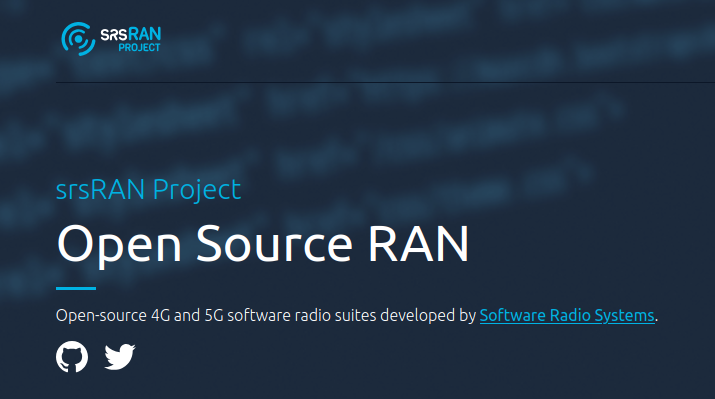
\includegraphics[keepaspectratio]{pictures/srsran.png}}

\subsection{Installation rapide via PPA
(Ubuntu)}\label{installation-rapide-via-ppa-ubuntu}

\begin{Shaded}
\begin{Highlighting}[]
\FunctionTok{sudo}\NormalTok{ apt update}
\FunctionTok{sudo}\NormalTok{ apt install }\AttributeTok{{-}y}\NormalTok{ software{-}properties{-}common}
\FunctionTok{sudo}\NormalTok{ add{-}apt{-}repository ppa:srsran/ppa}
\FunctionTok{sudo}\NormalTok{ apt update}
\FunctionTok{sudo}\NormalTok{ apt install }\AttributeTok{{-}y}\NormalTok{ srsran}
\end{Highlighting}
\end{Shaded}

\textbf{Vérifie l'install :}

\begin{Shaded}
\begin{Highlighting}[]
\ExtensionTok{srsenb} \AttributeTok{{-}{-}version}
\end{Highlighting}
\end{Shaded}

\begin{center}\rule{0.5\linewidth}{0.5pt}\end{center}

\subsection{Compilation depuis les
sources}\label{compilation-depuis-les-sources}

\begin{Shaded}
\begin{Highlighting}[]
\FunctionTok{sudo}\NormalTok{ apt update}
\FunctionTok{sudo}\NormalTok{ apt install }\AttributeTok{{-}y}\NormalTok{ git cmake build{-}essential libfftw3{-}dev libmbedtls{-}dev }\DataTypeTok{\textbackslash{}}
\NormalTok{  libboost{-}program{-}options{-}dev libconfig++{-}dev libsctp{-}dev }\DataTypeTok{\textbackslash{}}
\NormalTok{  libuhd{-}dev libpcsclite{-}dev pkg{-}config python3 python3{-}pip}

\FunctionTok{git}\NormalTok{ clone https://github.com/srsran/srsRAN\_Project.git}
\BuiltInTok{cd}\NormalTok{ srsRAN\_Project}
\FunctionTok{mkdir}\NormalTok{ build }\KeywordTok{\&\&} \BuiltInTok{cd}\NormalTok{ build}
\FunctionTok{cmake}\NormalTok{ ../}
\FunctionTok{make} \AttributeTok{{-}j}\VariableTok{$(}\FunctionTok{nproc}\VariableTok{)}
\FunctionTok{sudo}\NormalTok{ make install}
\end{Highlighting}
\end{Shaded}

\begin{center}\rule{0.5\linewidth}{0.5pt}\end{center}

\subsection{Générer/Configurer une SIM (IMSI, Ki,
OPC)}\label{guxe9nuxe9rerconfigurer-une-sim-imsi-ki-opc}

Pour connecter un téléphone réel ou un UE logiciel, il faut une SIM dont
les paramètres sont connus du core \textbf{srsEPC}.

\subsection{a. Générer un profil SIM
standard}\label{a.-guxe9nuxe9rer-un-profil-sim-standard}

\begin{itemize}
\tightlist
\item
  \textbf{IMSI} : identifiant unique (ex: \texttt{001010123456789})
\item
  \textbf{Ki} : clé de 16 octets (ex:
  \texttt{00112233445566778899aabbccddeeff})
\item
  \textbf{OPC} : clé d'opérateur de 16 octets (ex:
  \texttt{0102030405060708090a0b0c0d0e0f10})
\item
  \textbf{MSISDN} (optionnel) : numéro de tel virtuel
\end{itemize}

Tu peux utiliser un générateur en ligne
(\href{https://free5gc.org/webconsole/sim.html}{Free5GC SIM Generator}),
ou générer aléatoirement\,:

\begin{Shaded}
\begin{Highlighting}[]
\CommentTok{\# Générer un IMSI au hasard}
\VariableTok{IMSI}\OperatorTok{=}\StringTok{"001010}\VariableTok{$(}\FunctionTok{shuf} \AttributeTok{{-}i}\NormalTok{ 100000000{-}999999999 }\AttributeTok{{-}n}\NormalTok{ 1}\VariableTok{)}\StringTok{"}
\CommentTok{\# Générer une clé Ki et OPC}
\VariableTok{KI}\OperatorTok{=}\VariableTok{$(}\ExtensionTok{openssl}\NormalTok{ rand }\AttributeTok{{-}hex}\NormalTok{ 16}\VariableTok{)}
\VariableTok{OPC}\OperatorTok{=}\VariableTok{$(}\ExtensionTok{openssl}\NormalTok{ rand }\AttributeTok{{-}hex}\NormalTok{ 16}\VariableTok{)}
\BuiltInTok{echo} \StringTok{"IMSI: }\VariableTok{$IMSI}\StringTok{"}
\BuiltInTok{echo} \StringTok{"KI:   }\VariableTok{$KI}\StringTok{"}
\BuiltInTok{echo} \StringTok{"OPC:  }\VariableTok{$OPC}\StringTok{"}
\end{Highlighting}
\end{Shaded}

\subsection{b. Ajouter l'abonné dans
srsEPC}\label{b.-ajouter-labonnuxe9-dans-srsepc}

Ouvre le fichier de conf des abonnés, typiquement :

\begin{Shaded}
\begin{Highlighting}[]
\FunctionTok{nano}\NormalTok{ /etc/srsran/epc\_user\_db.csv}
\end{Highlighting}
\end{Shaded}

Ou dans ton dossier local \texttt{srsRAN\_Project/config/user\_db.csv}

\textbf{Exemple d'entrée :}

\begin{verbatim}
IMSI,  Ki,                       OPC,                      MSISDN,     AMF,   SQN
001010123456789,00112233445566778899aabbccddeeff,0102030405060708090a0b0c0d0e0f10,1234567890,8000,000000
\end{verbatim}

\textbf{Champ obligatoire}\,: IMSI, Ki, OPC (les autres = valeur par
défaut si besoin).

\begin{center}\rule{0.5\linewidth}{0.5pt}\end{center}

\subsection{Programmer une carte SIM réelle
(optionnel)}\label{programmer-une-carte-sim-ruxe9elle-optionnel}

Si tu utilises une carte programmable (Sysmocom, MagicSIM, etc.)\,:

\begin{itemize}
\tightlist
\item
  Utilise \href{https://github.com/osmocom/pysim}{pySIM} (Python)
\item
  Lance\,:
\end{itemize}

\begin{Shaded}
\begin{Highlighting}[]
\ExtensionTok{pysim{-}prog.py} \AttributeTok{{-}{-}ki} \VariableTok{$KI} \AttributeTok{{-}{-}opc} \VariableTok{$OPC} \AttributeTok{{-}{-}imsi} \VariableTok{$IMSI}
\end{Highlighting}
\end{Shaded}

(Adapté selon ton lecteur et modèle de carte)

\begin{center}\rule{0.5\linewidth}{0.5pt}\end{center}

\subsection{Lancer srsENB (eNodeB) et srsEPC
(core)}\label{lancer-srsenb-enodeb-et-srsepc-core}

Dans deux terminaux\,:

\begin{Shaded}
\begin{Highlighting}[]
\CommentTok{\# Terminal 1 (eNodeB)}
\ExtensionTok{srsenb}\NormalTok{ enb.conf}

\CommentTok{\# Terminal 2 (EPC)}
\ExtensionTok{srsepc}\NormalTok{ epc.conf}
\end{Highlighting}
\end{Shaded}

\begin{center}\rule{0.5\linewidth}{0.5pt}\end{center}

\subsection{Tester l'attachement UE}\label{tester-lattachement-ue}

\begin{itemize}
\tightlist
\item
  Allume ton téléphone (SIM insérée, mode réseau ``4G/auto'')
\item
  Vérifie la détection dans les logs
\item
  Si besoin, ajuste le PLMN dans \texttt{enb.conf} et \texttt{epc.conf}
  pour matcher l'IMSI de la SIM (ex: MCC/MNC = 001/01)
\end{itemize}

\begin{center}\rule{0.5\linewidth}{0.5pt}\end{center}

\subsubsection{Docs utiles}\label{docs-utiles}

\begin{itemize}
\tightlist
\item
  \url{https://docs.srsran.com/projects/4g/en/latest/index.html}
\item
  \url{https://osmocom.org/projects/pysim/wiki}
\end{itemize}

\section{L'évolution 5G : rupture technologique, nouveaux
usages}\label{luxe9volution-5g-rupture-technologique-nouveaux-usages}

\subsection{Objectifs et rupture de la
5G}\label{objectifs-et-rupture-de-la-5g}

\begin{itemize}
\tightlist
\item
  \textbf{Débit x10 à x100 par rapport à la 4G} (jusqu'à 10 Gbps en
  pointe, 1 Gbps courant)
\item
  \textbf{Ultra faible latence} (\textless\,1 ms possible)
\item
  \textbf{Connectivité massive} : jusqu'à 1 million d'objets/km² (IoT,
  capteurs, véhicules)
\item
  \textbf{Fiabilité et disponibilité quasi temps réel} (industrie,
  santé, véhicules autonomes)
\item
  \textbf{Flexibilité réseau} : découpage ``network slicing'', chaque
  usage a son ``mini-réseau'' dédié
\end{itemize}

\begin{center}\rule{0.5\linewidth}{0.5pt}\end{center}

\subsection{Ruptures techniques
majeures}\label{ruptures-techniques-majeures}

\begin{itemize}
\tightlist
\item
  \textbf{Nouvelles bandes de fréquences} : ajout du spectre
  millimétrique (\textgreater24 GHz), plus de capacité mais portée plus
  courte
\item
  \textbf{Massive MIMO} : dizaines/centaines d'antennes pour booster
  débit et couverture
\item
  \textbf{Beamforming} : orientation dynamique du signal vers chaque
  utilisateur
\item
  \textbf{Core 5G tout IP/cloud natif} : virtualisation (NFV), fonctions
  réseau en software (SDN)
\item
  \textbf{Architecture Standalone (SA)} : cœur 5G indépendant, vs
  Non-Standalone (NSA) où la 5G s'appuie sur la 4G
\end{itemize}

\begin{center}\rule{0.5\linewidth}{0.5pt}\end{center}

\subsection{Nouveaux usages rendus
possibles}\label{nouveaux-usages-rendus-possibles}

\begin{itemize}
\tightlist
\item
  \textbf{Internet mobile ultra haut débit} (streaming 4K/8K, réalité
  augmentée/virtuelle, cloud gaming)
\item
  \textbf{Industrie 4.0} : automatisation, robotique, maintenance
  prédictive, réseaux privés d'usine
\item
  \textbf{Véhicules connectés et autonomes} : communication V2X temps
  réel
\item
  \textbf{Santé} : télémédecine en temps réel, chirurgie à distance
\item
  \textbf{Smart Cities et IoT massif} : gestion d'énergie, surveillance,
  transports, capteurs urbains
\end{itemize}

\begin{center}\rule{0.5\linewidth}{0.5pt}\end{center}

\subsection{Limites, critiques et
défis}\label{limites-critiques-et-duxe9fis}

\begin{itemize}
\tightlist
\item
  \textbf{Couverture inégale} (surtout en mmWave, portée faible, besoin
  de micro-cellules)
\item
  \textbf{Consommation énergétique} (optimisée par le slicing mais
  déploiement massif d'antennes)
\item
  \textbf{Nouveaux risques de sécurité} (surface d'attaque plus large,
  virtualisation du cœur réseau)
\item
  \textbf{Investissements lourds} (infrastructures, renouvellement
  terminaux)
\end{itemize}

\begin{center}\rule{0.5\linewidth}{0.5pt}\end{center}

\subsection{Tableau récapitulatif}\label{tableau-ruxe9capitulatif}

\begin{longtable}[]{@{}
  >{\raggedright\arraybackslash}p{(\linewidth - 10\tabcolsep) * \real{0.1020}}
  >{\raggedright\arraybackslash}p{(\linewidth - 10\tabcolsep) * \real{0.1939}}
  >{\raggedright\arraybackslash}p{(\linewidth - 10\tabcolsep) * \real{0.0918}}
  >{\raggedright\arraybackslash}p{(\linewidth - 10\tabcolsep) * \real{0.1429}}
  >{\raggedright\arraybackslash}p{(\linewidth - 10\tabcolsep) * \real{0.1429}}
  >{\raggedright\arraybackslash}p{(\linewidth - 10\tabcolsep) * \real{0.3265}}@{}}
\toprule\noalign{}
\begin{minipage}[b]{\linewidth}\raggedright
Génération
\end{minipage} & \begin{minipage}[b]{\linewidth}\raggedright
Débit max
\end{minipage} & \begin{minipage}[b]{\linewidth}\raggedright
Latence
\end{minipage} & \begin{minipage}[b]{\linewidth}\raggedright
Connexions/km²
\end{minipage} & \begin{minipage}[b]{\linewidth}\raggedright
Architecture
\end{minipage} & \begin{minipage}[b]{\linewidth}\raggedright
Usages clés
\end{minipage} \\
\midrule\noalign{}
\endhead
\bottomrule\noalign{}
\endlastfoot
4G & \textasciitilde100 Mbps -- 1 Gbps & \textasciitilde50 ms &
\textasciitilde100\,000 & Tout-IP & Vidéo, web, app mobile \\
\textbf{5G} & 1--10 Gbps & \textless\,1--10 ms & 1\,000\,000+ & Cloud,
slicing & IoT massif, VR/AR, Industrie 4.0 \\
\end{longtable}

\begin{center}\rule{0.5\linewidth}{0.5pt}\end{center}

\subsection{À retenir}\label{uxe0-retenir}

\begin{quote}
\textbf{La 5G n'est pas juste ``plus rapide''}\,: elle transforme
l'infrastructure, permet l'émergence de nouveaux usages critiques
(industrie, santé, véhicules), et prépare le terrain pour un monde
ultra-connecté, piloté en temps réel.
\end{quote}

\section{5G SA labo\,: srsRAN Project + Open5GS (Ubuntu
2024)}\label{g-sa-labo-srsran-project-open5gs-ubuntu-2024}

\subsection{Prérequis}\label{pruxe9requis-1}

\begin{itemize}
\tightlist
\item
  \textbf{OS\,:} Ubuntu 22.04 ou 24.04 (x86\_64)
\item
  \textbf{Matériel\,:} SDR (USRP B200/B210/X300/PlutoSDR/LimeSDR\ldots)
  \emph{OU} mode simulation (aucun matériel SDR requis)
\item
  \textbf{Packages de base\,:} git, cmake, build-essential, etc.
\end{itemize}

\begin{center}\rule{0.5\linewidth}{0.5pt}\end{center}

\subsection{Installer Open5GS (Core
5G)}\label{installer-open5gs-core-5g}

\pandocbounded{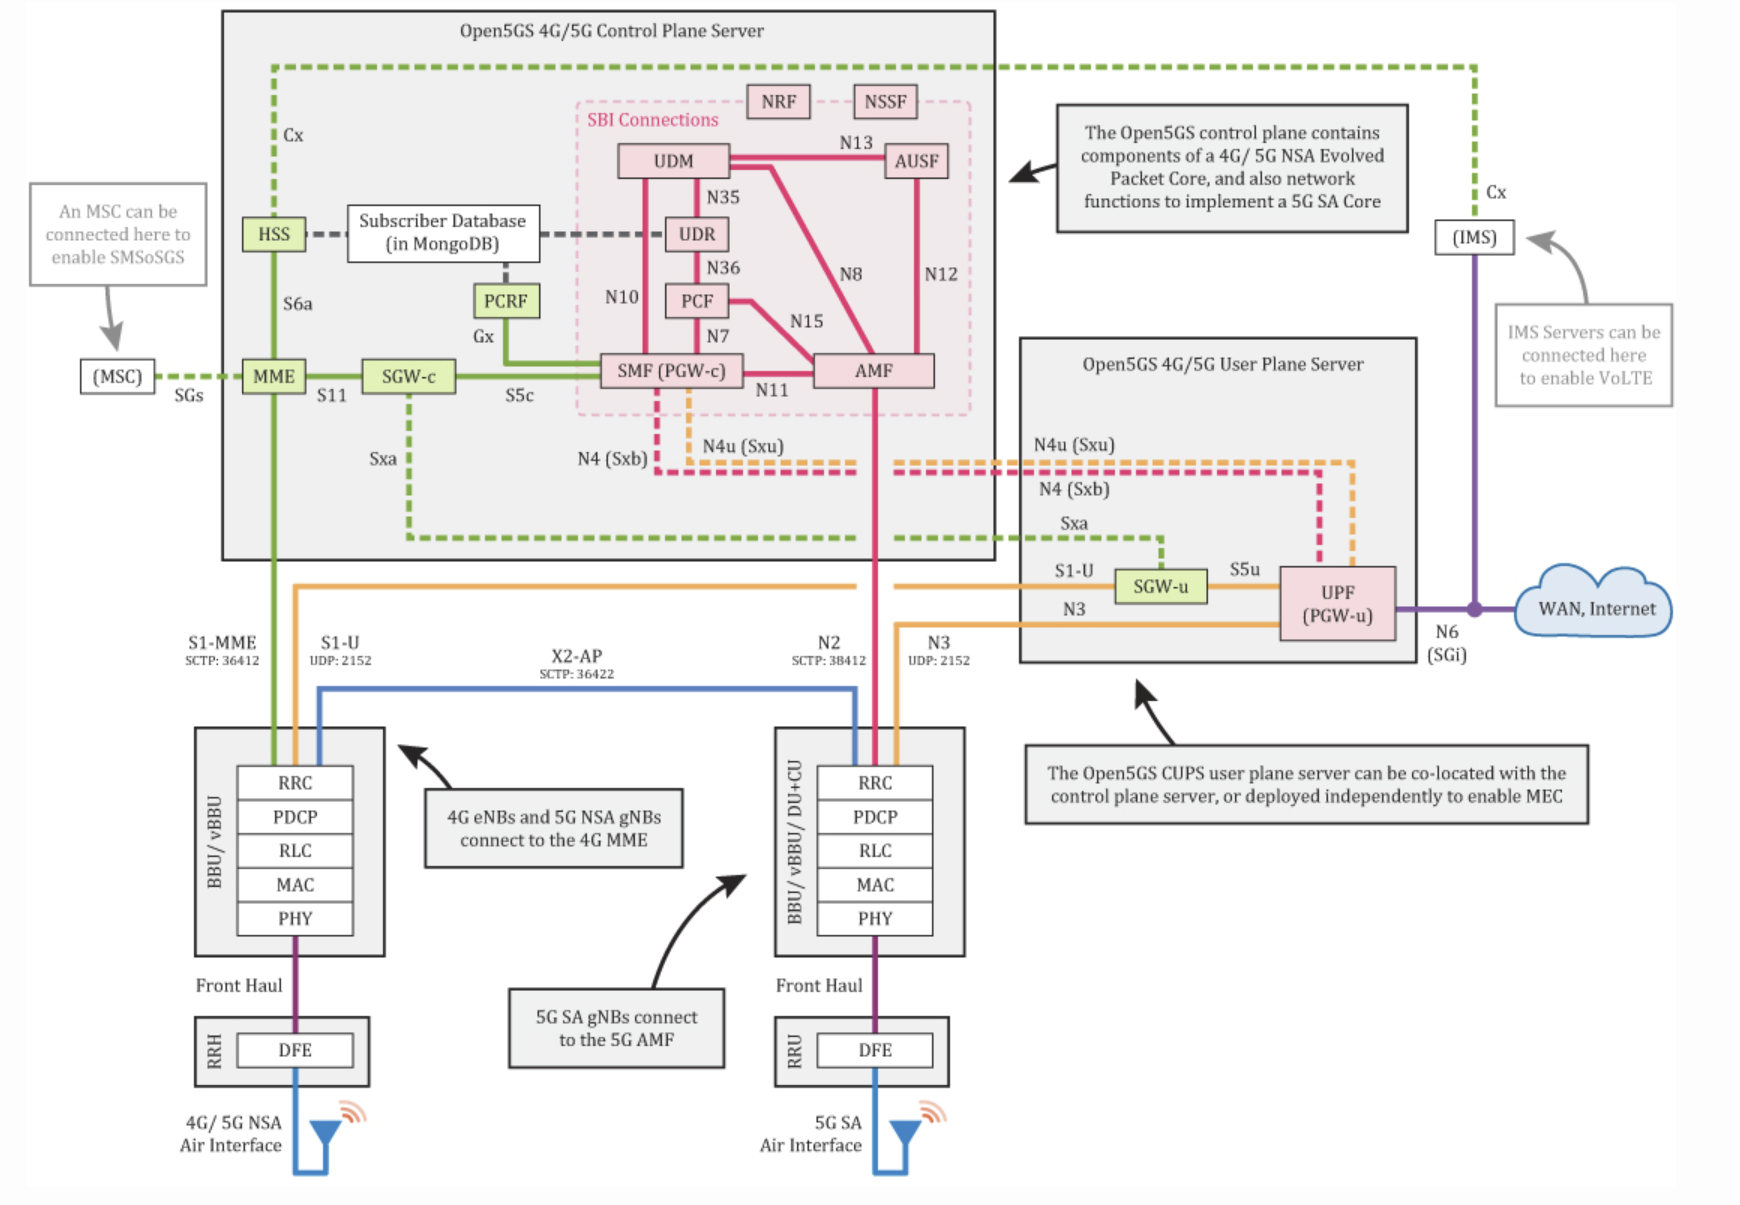
\includegraphics[keepaspectratio]{pictures/open5gs.png}}

\subsubsection{a) Dépendances}\label{a-duxe9pendances}

\begin{Shaded}
\begin{Highlighting}[]
\FunctionTok{sudo}\NormalTok{ apt update}
\FunctionTok{sudo}\NormalTok{ apt install }\AttributeTok{{-}y}\NormalTok{ git build{-}essential meson ninja{-}build python3 python3{-}pip python3{-}setuptools }\DataTypeTok{\textbackslash{}}
\NormalTok{  flex bison libsctp{-}dev libssl{-}dev libnghttp2{-}dev libmicrohttpd{-}dev }\DataTypeTok{\textbackslash{}}
\NormalTok{  libyaml{-}dev libmariadb{-}dev libmongoc{-}dev libbson{-}dev mongodb}
\end{Highlighting}
\end{Shaded}

\subsubsection{b) Cloner et compiler
Open5GS}\label{b-cloner-et-compiler-open5gs}

\begin{Shaded}
\begin{Highlighting}[]
\FunctionTok{git}\NormalTok{ clone https://github.com/open5gs/open5gs}
\BuiltInTok{cd}\NormalTok{ open5gs}
\ExtensionTok{meson}\NormalTok{ build }\AttributeTok{{-}{-}prefix}\OperatorTok{=}\KeywordTok{\textasciigrave{}}\BuiltInTok{pwd}\KeywordTok{\textasciigrave{}}\NormalTok{/install}
\ExtensionTok{ninja} \AttributeTok{{-}C}\NormalTok{ build}
\ExtensionTok{ninja} \AttributeTok{{-}C}\NormalTok{ build install}
\end{Highlighting}
\end{Shaded}

\emph{(Binaires dans \texttt{open5gs/install/bin/})}

\begin{center}\rule{0.5\linewidth}{0.5pt}\end{center}

\subsection{Installer srsRAN Project
(gNB/UE)}\label{installer-srsran-project-gnbue}

\subsubsection{a) Dépendances}\label{a-duxe9pendances-1}

\begin{Shaded}
\begin{Highlighting}[]
\FunctionTok{sudo}\NormalTok{ apt install }\AttributeTok{{-}y}\NormalTok{ cmake g++ libsctp{-}dev libfftw3{-}dev libmbedtls{-}dev }\DataTypeTok{\textbackslash{}}
\NormalTok{  libboost{-}program{-}options{-}dev libconfig++{-}dev pkg{-}config python3 python3{-}pip }\DataTypeTok{\textbackslash{}}
\NormalTok{  libzmq3{-}dev libpcsclite{-}dev}
\end{Highlighting}
\end{Shaded}

\subsubsection{b) Cloner et compiler
srsRAN}\label{b-cloner-et-compiler-srsran}

\begin{Shaded}
\begin{Highlighting}[]
\FunctionTok{git}\NormalTok{ clone https://github.com/srsran/srsRAN\_Project.git}
\BuiltInTok{cd}\NormalTok{ srsRAN\_Project}
\FunctionTok{mkdir}\NormalTok{ build }\KeywordTok{\&\&} \BuiltInTok{cd}\NormalTok{ build}
\FunctionTok{cmake}\NormalTok{ ../}
\FunctionTok{make} \AttributeTok{{-}j}\VariableTok{$(}\FunctionTok{nproc}\VariableTok{)}
\FunctionTok{sudo}\NormalTok{ make install}
\end{Highlighting}
\end{Shaded}

\emph{(Binaires dans \texttt{/usr/local/bin/})}

\begin{center}\rule{0.5\linewidth}{0.5pt}\end{center}

\subsection{Configurer Open5GS (Core)}\label{configurer-open5gs-core}

\begin{itemize}
\item
  Tous les fichiers\,: \texttt{open5gs/install/etc/open5gs/}
\item
  Fichiers clés\,:

  \begin{itemize}
  \tightlist
  \item
    \texttt{amf.yaml} (AMF/core)
  \item
    \texttt{smf.yaml} (SMF/session)
  \item
    \texttt{upf.yaml} (UPF/user-plane)
  \item
    \texttt{udm.yaml}, \texttt{ausf.yaml}, etc.
  \end{itemize}
\end{itemize}

\textbf{Edits minimaux\,:}

\begin{itemize}
\tightlist
\item
  PLMN\,: \texttt{mcc:\ 001}, \texttt{mnc:\ 01} (ou tes propres valeurs)
\item
  Dans \texttt{amf.yaml}\,: l'adresse \texttt{ngap} doit matcher celle
  de ton gNB (ex\,: \texttt{127.0.0.1})
\end{itemize}

\subsubsection{Ajouter un abonné test
(SIM)}\label{ajouter-un-abonnuxe9-test-sim}

\begin{itemize}
\item
  Ouvre \texttt{subscribers.yaml} ou passe par le
  \href{https://github.com/open5gs/open5gs/wiki/WebUI}{WebUI Open5GS}
\item
  Exemple d'entrée :

\begin{Shaded}
\begin{Highlighting}[]
\KeywordTok{{-}}\AttributeTok{ }\FunctionTok{imsi}\KeywordTok{:}\AttributeTok{ }\StringTok{\textquotesingle{}001010123456789\textquotesingle{}}
\AttributeTok{  }\FunctionTok{key}\KeywordTok{:}\AttributeTok{ }\StringTok{\textquotesingle{}465B5CE8B199B49FAA5F0A2EE238A6BC\textquotesingle{}}
\AttributeTok{  }\FunctionTok{opc}\KeywordTok{:}\AttributeTok{ }\StringTok{\textquotesingle{}E8ED289DEBA952E4283B54E88E6183CA\textquotesingle{}}
\AttributeTok{  }\FunctionTok{amf}\KeywordTok{:}\AttributeTok{ }\StringTok{\textquotesingle{}8000\textquotesingle{}}
\AttributeTok{  }\FunctionTok{sqn}\KeywordTok{:}\AttributeTok{ }\StringTok{\textquotesingle{}000000000000\textquotesingle{}}
\end{Highlighting}
\end{Shaded}
\item
  À reporter dans la SIM (physique ou config UE logicielle)
\end{itemize}

\begin{center}\rule{0.5\linewidth}{0.5pt}\end{center}

\subsection{Configurer srsRAN gNB}\label{configurer-srsran-gnb}

\begin{itemize}
\tightlist
\item
  Fichier\,: \texttt{srsran\_project/config/gnb.yaml} \emph{(ou
  \texttt{gnb.conf} selon la version)}
\end{itemize}

Exemple minimal\,:

\begin{Shaded}
\begin{Highlighting}[]
\FunctionTok{plmn}\KeywordTok{:}
\AttributeTok{  }\FunctionTok{mcc}\KeywordTok{:}\AttributeTok{ }\DecValTok{001}
\AttributeTok{  }\FunctionTok{mnc}\KeywordTok{:}\AttributeTok{ }\DecValTok{01}
\FunctionTok{amf}\KeywordTok{:}
\AttributeTok{  }\FunctionTok{addr}\KeywordTok{:}\AttributeTok{ }\FloatTok{127.0.0.1}\CommentTok{   \# IP du core Open5GS}
\AttributeTok{  }\FunctionTok{port}\KeywordTok{:}\AttributeTok{ }\DecValTok{38412}
\FunctionTok{slices}\KeywordTok{:}
\AttributeTok{  }\KeywordTok{{-}}\AttributeTok{ }\FunctionTok{sst}\KeywordTok{:}\AttributeTok{ }\DecValTok{1}
\AttributeTok{    }\FunctionTok{sd}\KeywordTok{:}\AttributeTok{ }\DecValTok{0x000001}
\end{Highlighting}
\end{Shaded}

\begin{itemize}
\tightlist
\item
  Spécifie \texttt{rf.device\_name} pour ton SDR (si RF)
\item
  Réseau/interface\,: ex\,: \texttt{ngap.interface\_name:\ lo} pour
  tests locaux
\end{itemize}

\begin{center}\rule{0.5\linewidth}{0.5pt}\end{center}

\subsection{Configurer srsRAN UE (si test en pur
logiciel)}\label{configurer-srsran-ue-si-test-en-pur-logiciel}

\begin{itemize}
\tightlist
\item
  Fichier\,: \texttt{srsran\_project/config/ue.yaml} \emph{(ou
  \texttt{ue.conf})}
\item
  Paramètres\,: PLMN, key, opc, amf, imei identiques à l'abonné Open5GS.
\item
  Mode RF ou simulation selon besoin.
\end{itemize}

\begin{center}\rule{0.5\linewidth}{0.5pt}\end{center}

\subsection{Lancer le Core Open5GS}\label{lancer-le-core-open5gs}

Ouvre \textbf{plusieurs terminaux} (ou \texttt{tmux})\,:

\begin{Shaded}
\begin{Highlighting}[]
\BuiltInTok{cd}\NormalTok{ open5gs/install/bin/}
\FunctionTok{sudo}\NormalTok{ ./open5gs{-}mmed}
\FunctionTok{sudo}\NormalTok{ ./open5gs{-}sgwcd}
\FunctionTok{sudo}\NormalTok{ ./open5gs{-}smfd}
\FunctionTok{sudo}\NormalTok{ ./open5gs{-}amfd}
\FunctionTok{sudo}\NormalTok{ ./open5gs{-}upfd}
\FunctionTok{sudo}\NormalTok{ ./open5gs{-}ausfd}
\FunctionTok{sudo}\NormalTok{ ./open5gs{-}udmd}
\FunctionTok{sudo}\NormalTok{ ./open5gs{-}pcfd}
\FunctionTok{sudo}\NormalTok{ ./open5gs{-}nrfd}
\FunctionTok{sudo}\NormalTok{ ./open5gs{-}bsfd}
\FunctionTok{sudo}\NormalTok{ ./open5gs{-}hssd}
\end{Highlighting}
\end{Shaded}

Ou tout-en-un :

\begin{Shaded}
\begin{Highlighting}[]
\FunctionTok{sudo}\NormalTok{ ./open5gs{-}daemon}
\end{Highlighting}
\end{Shaded}

\begin{center}\rule{0.5\linewidth}{0.5pt}\end{center}

\subsection{Lancer le gNB srsRAN}\label{lancer-le-gnb-srsran}

\begin{Shaded}
\begin{Highlighting}[]
\ExtensionTok{srsran\_gnb} \AttributeTok{{-}{-}cfg}\NormalTok{ srsran\_project/config/gnb.yaml}
\end{Highlighting}
\end{Shaded}

\begin{center}\rule{0.5\linewidth}{0.5pt}\end{center}

\subsection{(Optionnel) Lancer le srsUE (UE 5G SA
logiciel)}\label{optionnel-lancer-le-srsue-ue-5g-sa-logiciel}

\begin{Shaded}
\begin{Highlighting}[]
\ExtensionTok{srsran\_ue} \AttributeTok{{-}{-}cfg}\NormalTok{ srsran\_project/config/ue.yaml}
\end{Highlighting}
\end{Shaded}

Ou utiliser un vrai smartphone 5G + SDR côté réseau.

\begin{center}\rule{0.5\linewidth}{0.5pt}\end{center}

\subsection{Supervision}\label{supervision}

\begin{itemize}
\tightlist
\item
  Utilise le \textbf{WebUI Open5GS} (si installé) pour la gestion des
  SIM et le monitoring.
\item
  Surveille les logs (attach, registration, PDU session, etc.).
\item
  Une fois le UE attaché, fais un \texttt{ping} (depuis l'UE ou via
  l'interface UPF).
\end{itemize}

\begin{center}\rule{0.5\linewidth}{0.5pt}\end{center}

\subsection{Conseils de dépannage}\label{conseils-de-duxe9pannage}

\begin{itemize}
\tightlist
\item
  \textbf{PLMN, clés et IP doivent correspondre} partout.
\item
  Utilise \texttt{127.0.0.1} ou une IP locale réelle selon ton cas.
\item
  Avec du RF\,: vérifie fréquence/bande/SDR.
\item
  En simulation pure (``null device'') tu peux tout tester sans SDR.
\end{itemize}

\begin{center}\rule{0.5\linewidth}{0.5pt}\end{center}

\subsection{Liens utiles}\label{liens-utiles-2}

\begin{itemize}
\tightlist
\item
  \href{https://docs.srsran.com/projects/5g/en/latest/}{Docs srsRAN
  Project 5G}
\item
  \href{https://open5gs.org/open5gs/docs/}{Docs Open5GS}
\item
  \href{https://github.com/open5gs/open5gs/wiki/WebUI}{WebUI Open5GS}
\item
  \href{https://open5gs.org/open5gs/docs/guide-subscription/}{Guide
  abonnés Open5GS}
\end{itemize}

\section{LoRa et réseaux longue
portée}\label{lora-et-ruxe9seaux-longue-portuxe9e}

Les réseaux radio traditionnels, comme les réseaux cellulaires ou le
Wi-Fi, sont conçus pour transporter des volumes importants de données
avec des débits élevés.\\
Cependant, de nombreuses applications de l'Internet des objets (IoT)
nécessitent des caractéristiques différentes :

\begin{itemize}
\tightlist
\item
  très faible consommation énergétique
\item
  portée radio importante
\item
  faible volume de données
\item
  coût matériel réduit
\end{itemize}

La technologie \textbf{LoRa (Long Range)} a été conçue pour répondre à
ces besoins.

LoRa est une modulation radio développée par la société
\textbf{Semtech}, utilisée dans l'architecture réseau
\textbf{LoRaWAN}.\\
Cette technologie permet de transmettre des données sur plusieurs
kilomètres tout en conservant une consommation énergétique extrêmement
faible.

Les applications typiques incluent :

\begin{itemize}
\tightlist
\item
  capteurs environnementaux
\item
  agriculture connectée
\item
  suivi d'objets
\item
  capteurs industriels
\item
  réseaux de capteurs urbains
\end{itemize}

Dans ce chapitre, nous allons décrire :

\begin{enumerate}
\def\labelenumi{\arabic{enumi}.}
\tightlist
\item
  l'architecture d'un réseau LoRa
\item
  la configuration d'une gateway
\item
  l'enregistrement de capteurs et l'exploitation des données
\end{enumerate}

\begin{center}\rule{0.5\linewidth}{0.5pt}\end{center}

\subsection{Architecture d'un réseau
LoRa}\label{architecture-dun-ruxe9seau-lora}

Contrairement aux réseaux cellulaires traditionnels, les réseaux LoRaWAN
utilisent une architecture relativement simple.

Un réseau LoRa est composé de quatre éléments principaux :

\begin{itemize}
\tightlist
\item
  \textbf{End devices} (capteurs ou objets connectés)
\item
  \textbf{LoRa Gateway}
\item
  \textbf{Network Server}
\item
  \textbf{Application Server}
\end{itemize}

L'architecture générale peut être représentée par le diagramme suivant :

\href{assets/uml.png}{\pandocbounded{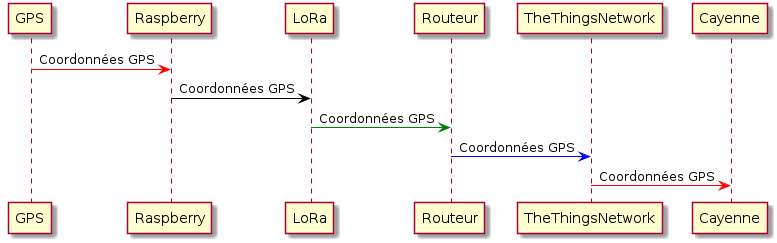
\includegraphics[keepaspectratio]{assets/uml.png}}}

Les capteurs LoRa transmettent leurs données par radio vers une
\textbf{gateway LoRa}.\\
Cette gateway agit comme un \textbf{pont entre le réseau radio et
Internet}.

Contrairement à une station de base cellulaire, la gateway LoRa ne
réalise pas de traitement complexe.\\
Elle agit principalement comme un \textbf{relai de paquets radio}.

Les données sont ensuite envoyées vers un \textbf{Network Server}, qui
se charge de :

\begin{itemize}
\tightlist
\item
  vérifier l'authentification des capteurs
\item
  supprimer les duplications de paquets
\item
  router les messages vers les applications
\end{itemize}

Dans de nombreux déploiements expérimentaux ou communautaires, le
serveur réseau utilisé est :

\textbf{The Things Network (TTN)}.

\begin{center}\rule{0.5\linewidth}{0.5pt}\end{center}

\subsubsection{Exemple de gateway LoRa}\label{exemple-de-gateway-lora}

Dans ce projet, une gateway \textbf{Dragino LoRa} a été utilisée.

\href{assets/WiFi_Dragino.png}{\pandocbounded{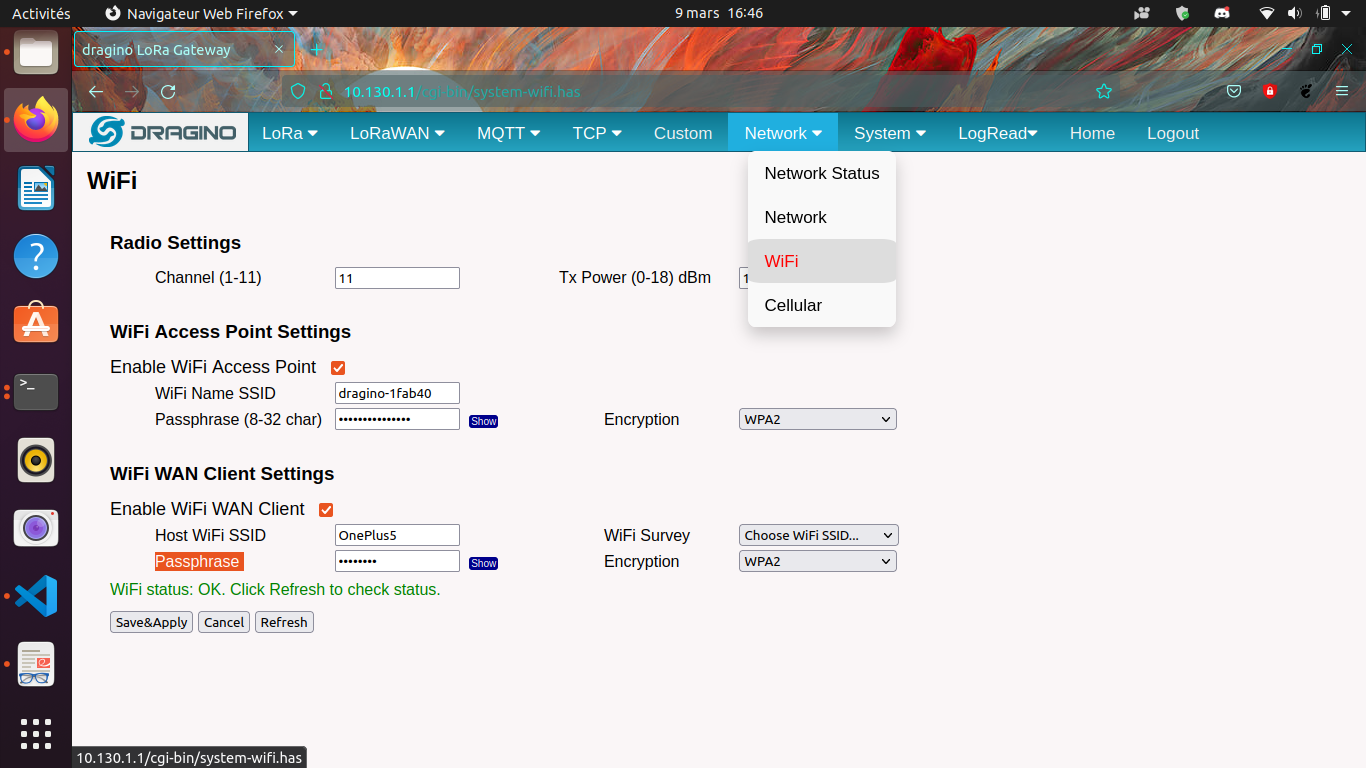
\includegraphics[keepaspectratio]{assets/WiFi_Dragino.png}}}

Cette gateway peut être connectée au réseau via :

\begin{itemize}
\tightlist
\item
  WiFi
\item
  Ethernet
\item
  modem cellulaire
\end{itemize}

Les données radio reçues sont encapsulées dans des paquets IP et
envoyées vers le serveur LoRaWAN.

\begin{center}\rule{0.5\linewidth}{0.5pt}\end{center}

\subsubsection{Configuration de la gateway
LoRa}\label{configuration-de-la-gateway-lora}

La première étape consiste à configurer la gateway pour qu'elle se
connecte au serveur \textbf{The Things Network}.

La configuration s'effectue généralement via une interface web
embarquée.

Les paramètres principaux sont :

\begin{itemize}
\tightlist
\item
  \textbf{fréquence radio}
\item
  \textbf{identifiant de la gateway}
\item
  \textbf{adresse du serveur LoRaWAN}
\end{itemize}

Voici un exemple d'interface de configuration :

\href{assets/config_gw_ttn.png}{\pandocbounded{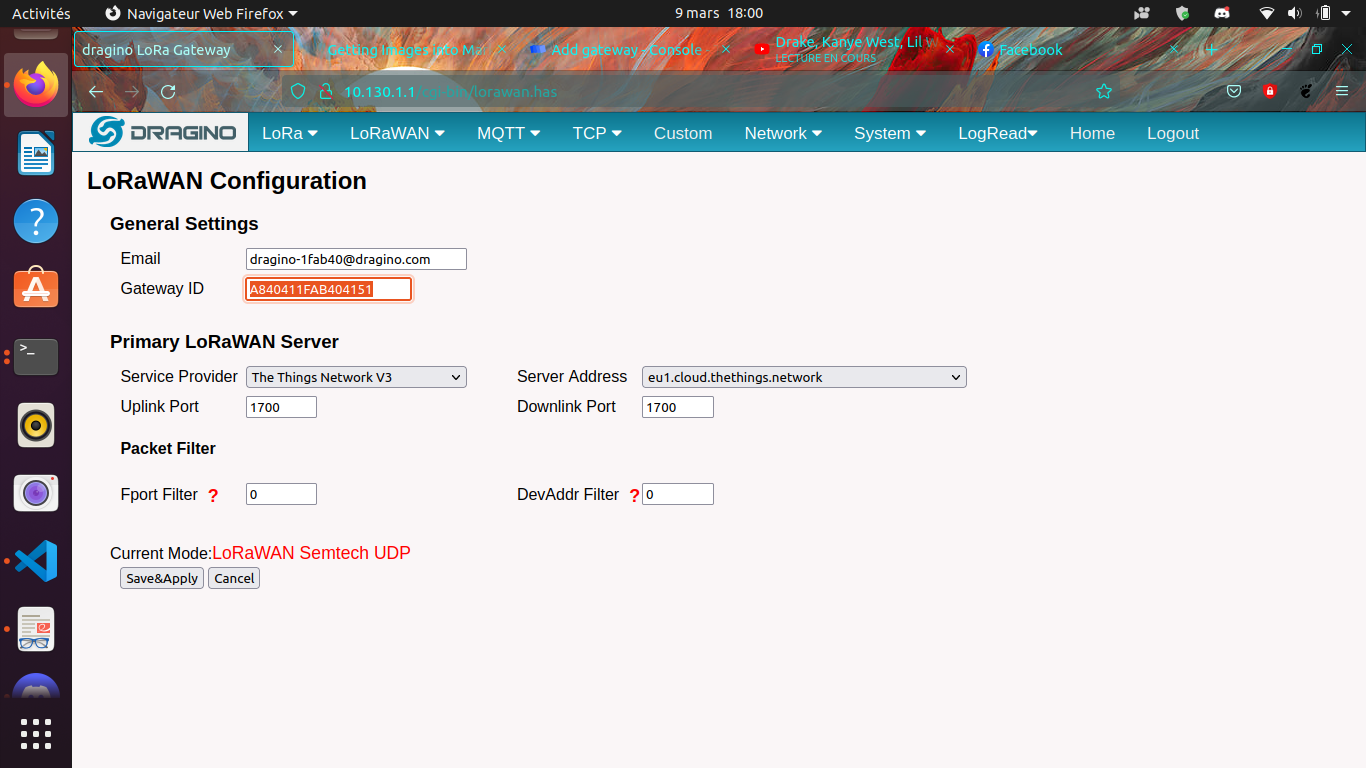
\includegraphics[keepaspectratio]{assets/config_gw_ttn.png}}}

Une fois la gateway configurée, elle doit être enregistrée sur la
plateforme TTN.

L'opération s'effectue via l'interface web de \textbf{The Things
Network}.

\href{assets/config_ttn_gw.png}{\pandocbounded{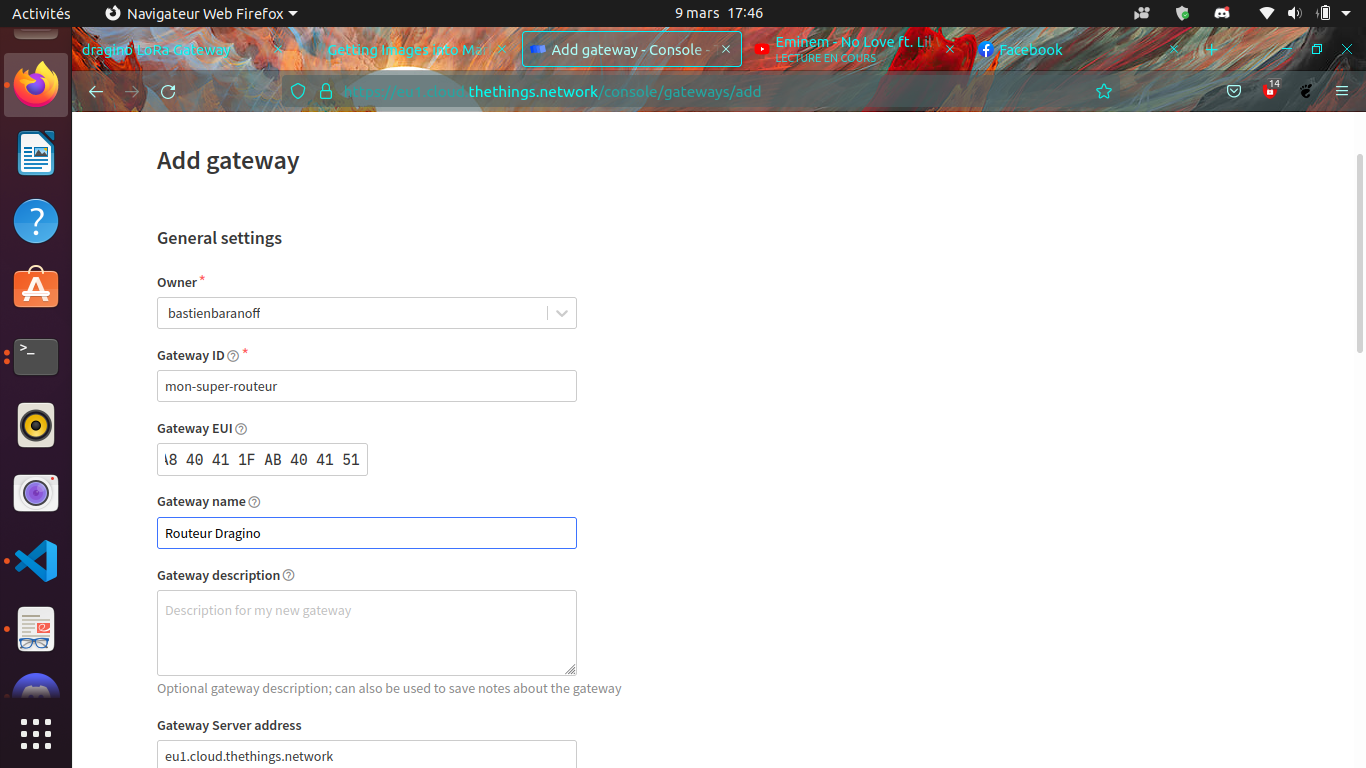
\includegraphics[keepaspectratio]{assets/config_ttn_gw.png}}}

Les informations nécessaires sont :

\begin{itemize}
\tightlist
\item
  Gateway ID
\item
  localisation géographique
\item
  fréquence utilisée
\end{itemize}

Ces informations permettent au réseau TTN d'intégrer la gateway dans son
infrastructure.

\begin{center}\rule{0.5\linewidth}{0.5pt}\end{center}

\subsubsection{Installation du système sur Raspberry
Pi}\label{installation-du-systuxe8me-sur-raspberry-pi}

Certaines gateways LoRa utilisent un \textbf{Raspberry Pi} comme système
embarqué.

Dans ce cas, il est nécessaire d'installer un système Linux sur la carte
SD.

Le système recommandé est généralement \textbf{Raspberry Pi OS}.

\href{assets/choose_os.png}{\pandocbounded{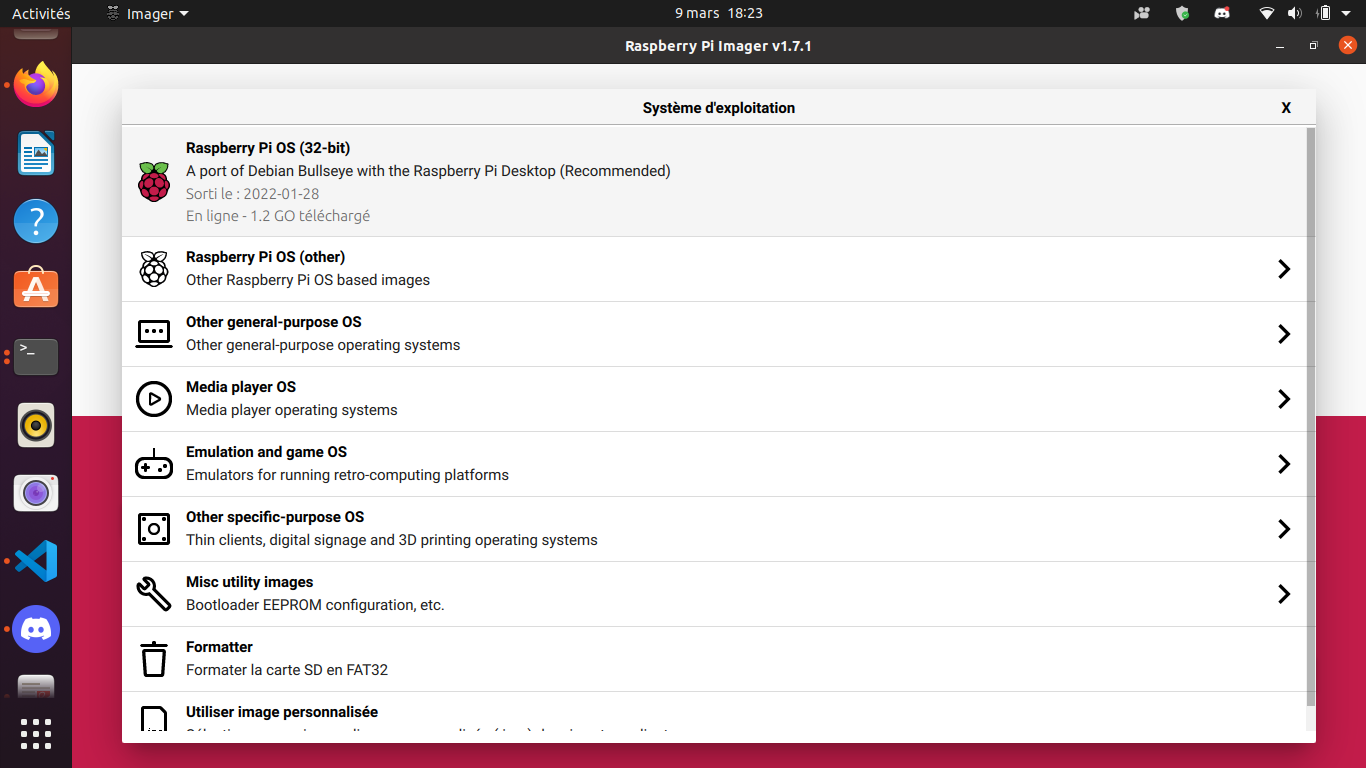
\includegraphics[keepaspectratio]{assets/choose_os.png}}}

La préparation de la carte SD peut être réalisée avec l'outil
\textbf{Raspberry Pi Imager}.

Une fois l'image sélectionnée, certaines options doivent être
configurées :

\begin{itemize}
\tightlist
\item
  accès SSH
\item
  configuration WiFi
\item
  utilisateur et mot de passe
\end{itemize}

\href{assets/options_sd_rpi.png}{\pandocbounded{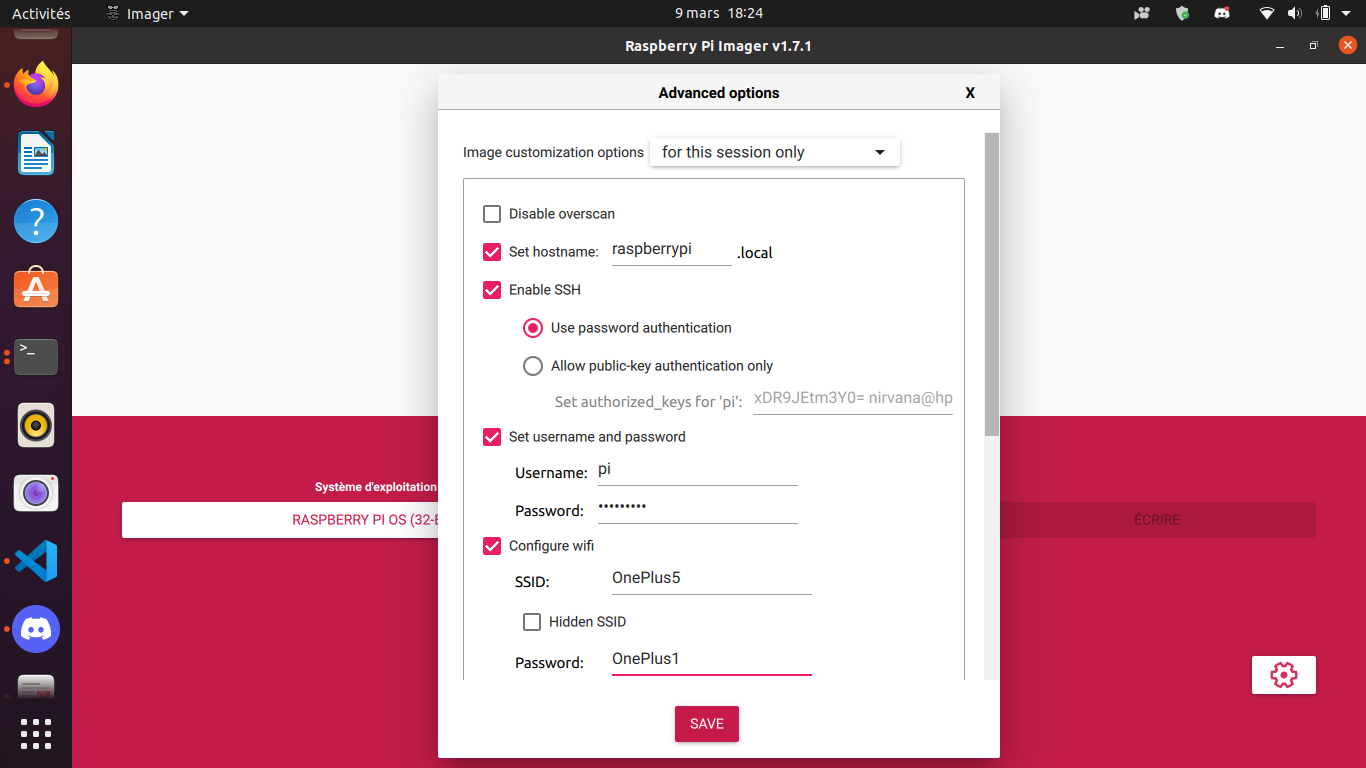
\includegraphics[keepaspectratio]{assets/options_sd_rpi.png}}}

Après l'installation, la gateway peut être configurée via SSH.

Exemple de connexion :

\begin{Shaded}
\begin{Highlighting}[]
\FunctionTok{ssh}\NormalTok{ pi@192.168.1.42}
\end{Highlighting}
\end{Shaded}

Mise à jour du système :

\begin{Shaded}
\begin{Highlighting}[]
\FunctionTok{sudo}\NormalTok{ apt update }\KeywordTok{\&\&} \DataTypeTok{\textbackslash{}}
\FunctionTok{sudo}\NormalTok{ apt upgrade }\AttributeTok{{-}y}
\end{Highlighting}
\end{Shaded}

Installation des outils nécessaires :

\begin{Shaded}
\begin{Highlighting}[]
\FunctionTok{sudo}\NormalTok{ apt install }\DataTypeTok{\textbackslash{}}
\NormalTok{    git }\DataTypeTok{\textbackslash{}}
\NormalTok{    build{-}essential }\DataTypeTok{\textbackslash{}}
\NormalTok{    python3 }\DataTypeTok{\textbackslash{}}
\NormalTok{    python3{-}pip}
\end{Highlighting}
\end{Shaded}

\begin{center}\rule{0.5\linewidth}{0.5pt}\end{center}

\subsubsection{Enregistrement des capteurs
LoRa}\label{enregistrement-des-capteurs-lora}

Une fois la gateway opérationnelle, il est possible d'ajouter des
\textbf{end devices} dans le réseau.

L'opération s'effectue depuis la console TTN.

\href{assets/add_enddevice.png}{\pandocbounded{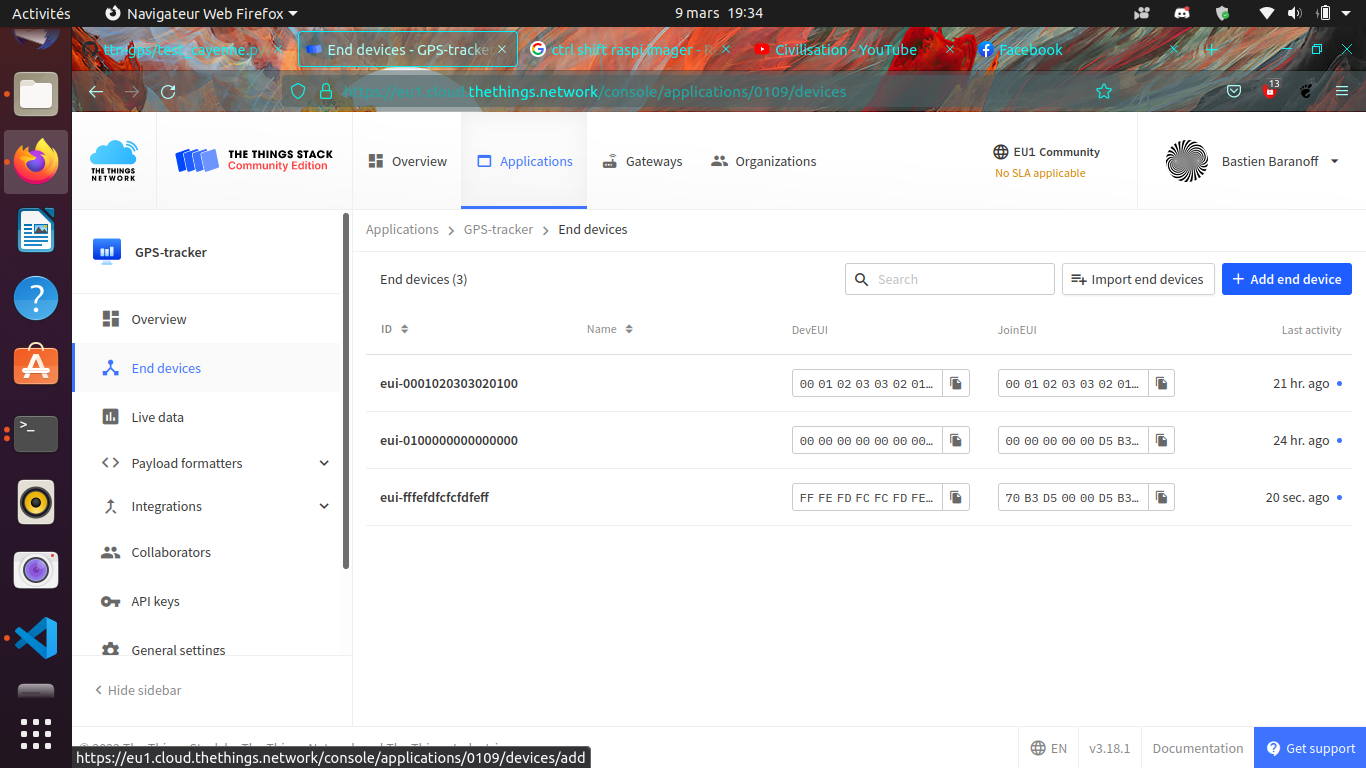
\includegraphics[keepaspectratio]{assets/add_enddevice.png}}}

Les paramètres nécessaires sont :

\begin{itemize}
\tightlist
\item
  \textbf{DevEUI}
\item
  \textbf{AppEUI}
\item
  \textbf{AppKey}
\end{itemize}

Ces identifiants permettent d'authentifier le capteur sur le réseau
LoRaWAN.

Une fois ces paramètres renseignés, l'appareil peut être enregistré.

\href{assets/register_enddevice.png}{\pandocbounded{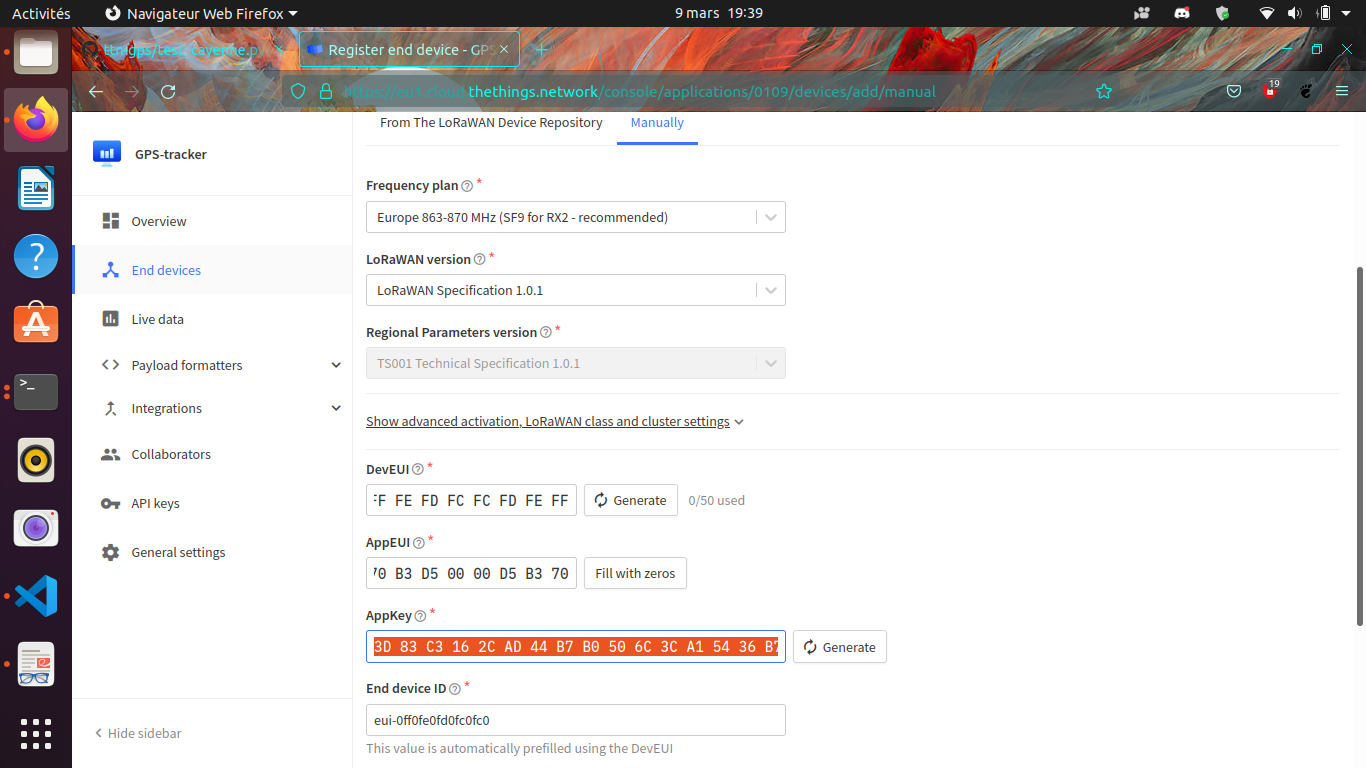
\includegraphics[keepaspectratio]{assets/register_enddevice.png}}}

\begin{center}\rule{0.5\linewidth}{0.5pt}\end{center}

\subsubsection{Encodage des données}\label{encodage-des-donnuxe9es}

Les données transmises par les capteurs LoRa sont généralement encodées
dans un format compact.

Un format largement utilisé est \textbf{Cayenne LPP (Low Power
Payload)}.

Ce format permet de représenter différents types de capteurs :

\begin{itemize}
\tightlist
\item
  température
\item
  humidité
\item
  pression
\item
  GPS
\item
  niveau de batterie
\end{itemize}

Exemple de format Cayenne :

\href{assets/format_cayenne.png}{\pandocbounded{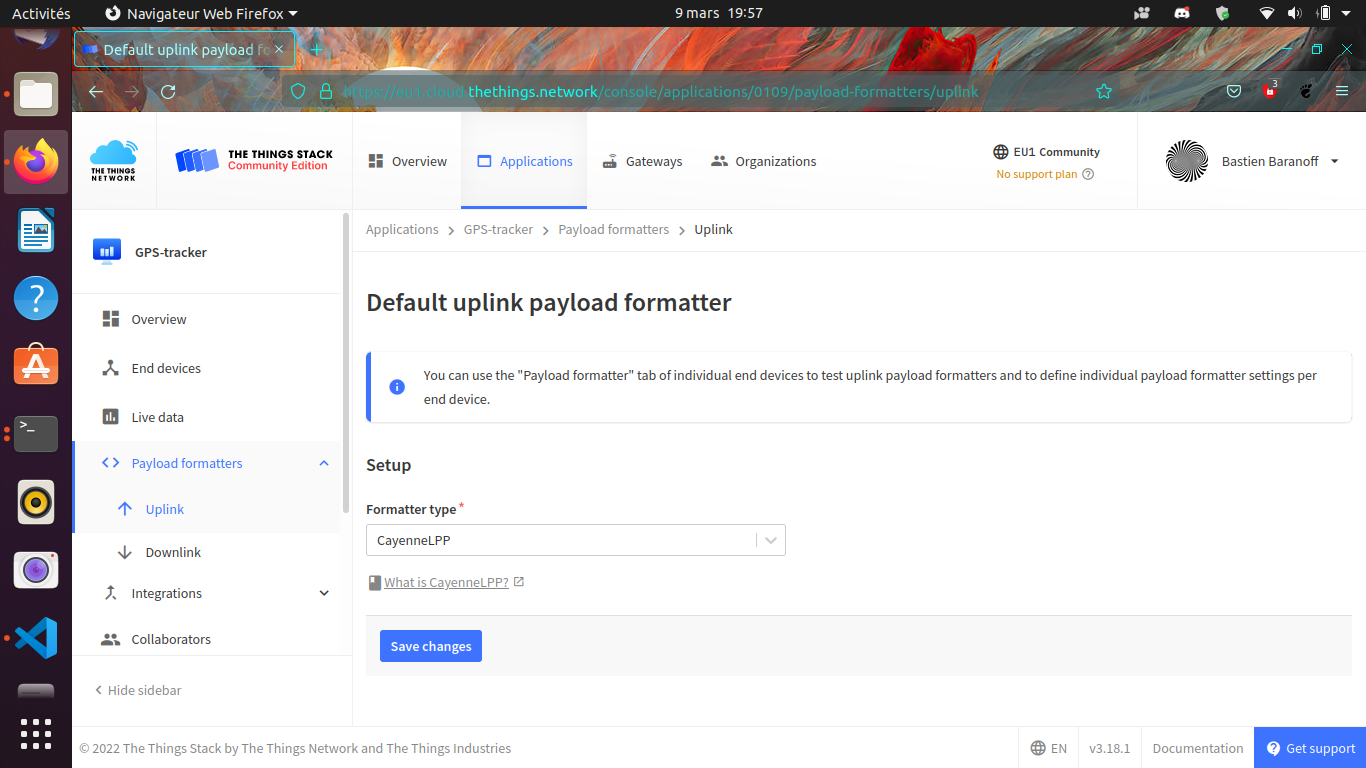
\includegraphics[keepaspectratio]{assets/format_cayenne.png}}}

Ce format facilite l'intégration avec les plateformes IoT.

\begin{center}\rule{0.5\linewidth}{0.5pt}\end{center}

\subsubsection{Configuration de l'application
TTN}\label{configuration-de-lapplication-ttn}

Pour recevoir les données du capteur, il est nécessaire de récupérer les
informations de connexion :

\href{assets/coordonnees_ttn.png}{\pandocbounded{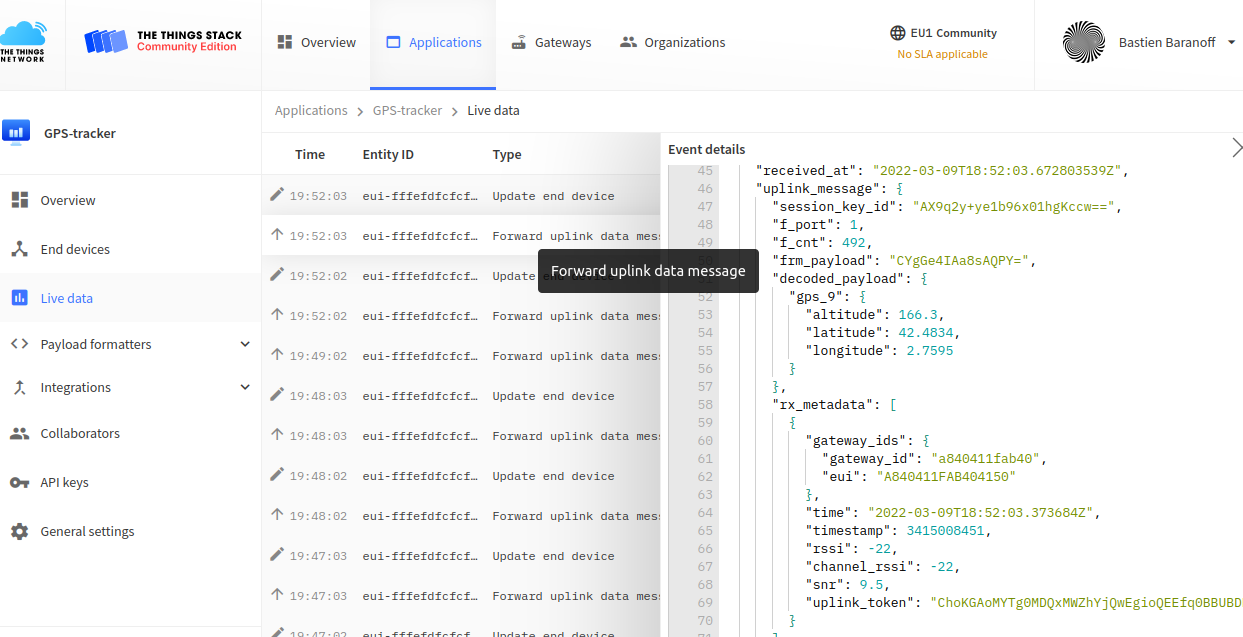
\includegraphics[keepaspectratio]{assets/coordonnees_ttn.png}}}

Ces informations incluent :

\begin{itemize}
\tightlist
\item
  identifiant d'application
\item
  clé d'accès
\item
  endpoint du serveur
\end{itemize}

\begin{center}\rule{0.5\linewidth}{0.5pt}\end{center}

\subsubsection{Visualisation des
données}\label{visualisation-des-donnuxe9es}

Les données LoRa peuvent être visualisées sur différentes plateformes
IoT.

Un exemple couramment utilisé est \textbf{Cayenne IoT}.

Ajout d'un nouvel appareil :

\href{assets/add_new_cayenne.png}{\pandocbounded{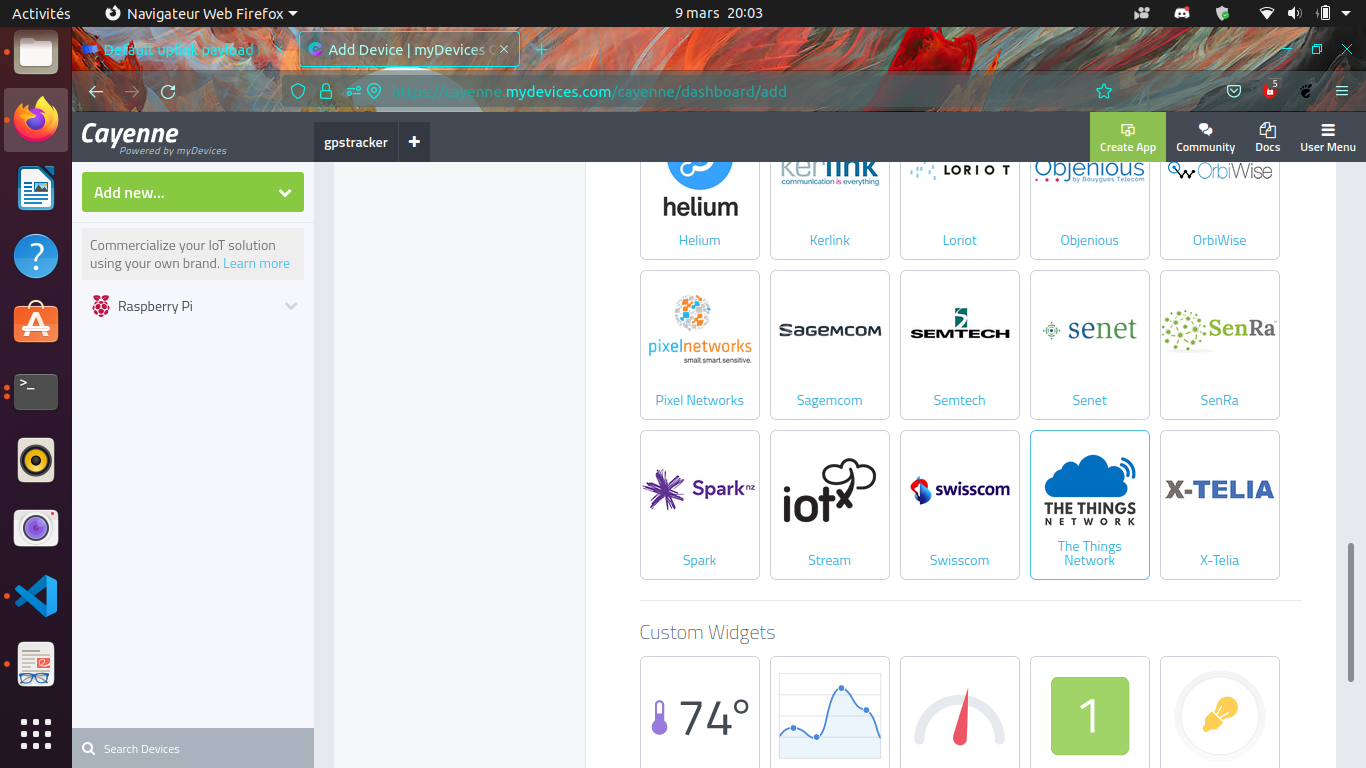
\includegraphics[keepaspectratio]{assets/add_new_cayenne.png}}}

Une fois le capteur connecté, les données peuvent être affichées sous
forme de tableaux ou de graphiques.

\href{assets/dragino_cayenne.png}{\pandocbounded{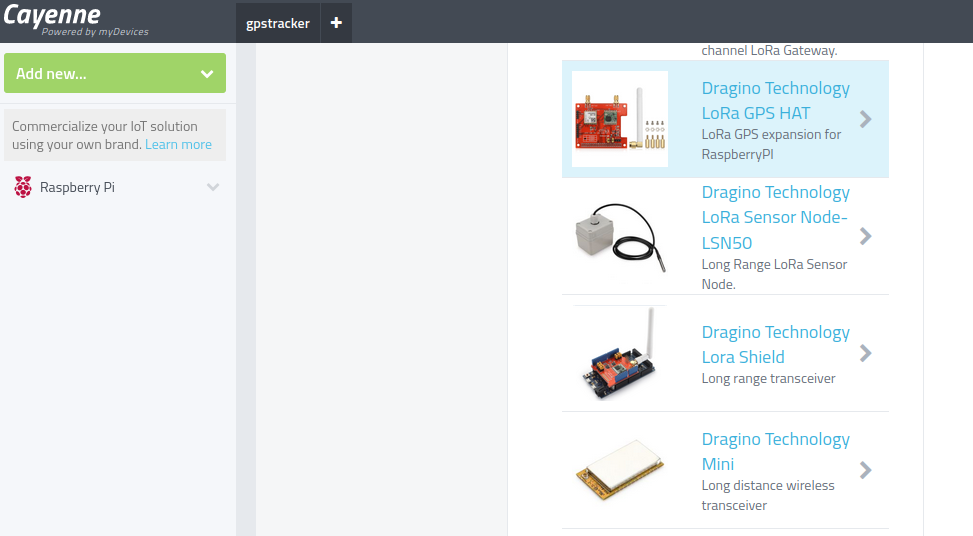
\includegraphics[keepaspectratio]{assets/dragino_cayenne.png}}}

Certains capteurs permettent également de transmettre des
\textbf{coordonnées GPS}.

Ces données peuvent être visualisées en temps réel sur une carte.

\href{assets/gps_live.png}{\pandocbounded{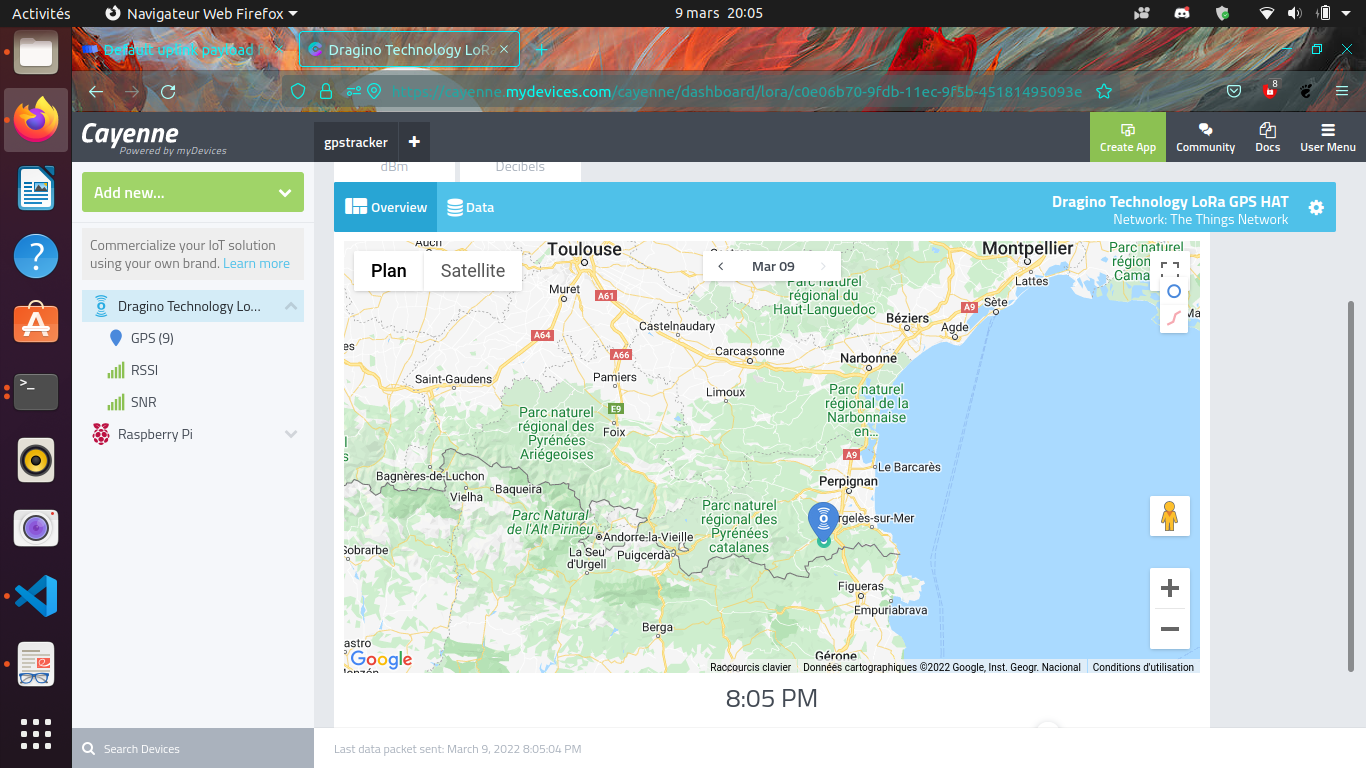
\includegraphics[keepaspectratio]{assets/gps_live.png}}}

\begin{center}\rule{0.5\linewidth}{0.5pt}\end{center}

\subsection{Conclusion}\label{conclusion-1}

Les réseaux LoRaWAN offrent une solution efficace pour connecter des
objets sur de longues distances avec une consommation énergétique très
faible.

Grâce à :

\begin{itemize}
\tightlist
\item
  une infrastructure radio simple
\item
  des gateways peu coûteuses
\item
  des plateformes open source comme TTN
\end{itemize}

il est possible de déployer rapidement un réseau IoT fonctionnel.

Cette technologie constitue aujourd'hui une composante importante de
l'écosystème \textbf{Internet des objets}, en complément des réseaux
cellulaires traditionnels.

\section{A5/1 --- Chiffrement GSM}\label{a51-chiffrement-gsm}

\textbf{A5/1} est l'algorithme de chiffrement à flot utilisé dans le GSM
pour assurer la confidentialité des communications radio entre le mobile
et la station de base (BTS).

\subsection{Principe de
fonctionnement}\label{principe-de-fonctionnement}

\begin{itemize}
\tightlist
\item
  \textbf{Chiffrement à flot} avec un état interne de 64 bits (3
  registres à décalage LFSR)
\item
  Initialisé avec la clé \textbf{Kc} (calculée à partir de la Ki de la
  SIM via l'algorithme A3/A8 et l'IMSI de l'abonné)
\item
  Le chiffrement s'applique en temps réel, bit par bit, sur la voix ou
  les données
\end{itemize}

\subsection{Vulnérabilités}\label{vulnuxe9rabilituxe9s}

\begin{itemize}
\tightlist
\item
  \textbf{Conception ancienne (années 1980/1990)}
\item
  Plusieurs attaques connues :

  \begin{itemize}
  \tightlist
  \item
    Tables arc-en-ciel (time-memory tradeoff, ex\,: Kraken/projet A5/1)
  \item
    Attaques sur les faiblesses des LFSR et synchronisation des
    registres
  \item
    Récupération de Kc si suffisamment de keystream est capturé
  \end{itemize}
\end{itemize}

\subsection{Outils open source}\label{outils-open-source}

\begin{itemize}
\tightlist
\item
  \href{https://opensource.srlabs.de/projects/a51-decrypt}{Kraken}
\item
  \href{https://github.com/ptrkrysik/gr-gsm}{gr-gsm + Airprobe}
\item
  \textbf{OsmocomBB} : possible d'injecter ou d'extraire des keystreams
  pour attaques bruteforce
\end{itemize}

\subsection{Détection \& tests}\label{duxe9tection-tests}

\begin{itemize}
\tightlist
\item
  Si la cellule envoie un «\,Ciphering Indicator\,», certains téléphones
  préviennent quand le chiffrement est désactivé
\item
  La plupart des réseaux modernes désactivent l'A5/1, passent en A5/3 ou
  désactivent complètement le chiffrement
\end{itemize}

\subsection{Pour aller plus loin}\label{pour-aller-plus-loin}

\begin{itemize}
\tightlist
\item
  \href{https://en.wikipedia.org/wiki/A5/1}{A5/1 sur Wikipédia}
\item
  \href{https://media.ccc.de/v/27c3-3894-en-breaking_gsm_with_rainbow_tables}{Attaques
  A5/1 (Karsten Nohl, CCC)}
\end{itemize}

\begin{center}\rule{0.5\linewidth}{0.5pt}\end{center}

\textbf{Note légale :}\\
Toute attaque ou rétro-ingénierie d'A5/1 est réservée à la recherche, au
pentesting autorisé, ou à la démonstration légale.\\
\textbf{L'interception non autorisée est illégale} dans la plupart des
pays.

\begin{center}\rule{0.5\linewidth}{0.5pt}\end{center}

\begin{itemize}
\tightlist
\item
  \textbf{Kraken}\,: outil de déchiffrement bruteforce A5/1 (GSM) via
  tables arc-en-ciel (rainbow tables).
\item
  \textbf{behemoth.py}\,: script Python (non officiel, communautaire)
  pour automatiser et paralléliser l'attaque Kraken, notamment sur de
  grandes infrastructures (ex\,: cluster, GPU, ou tâches batch).
\end{itemize}

\begin{center}\rule{0.5\linewidth}{0.5pt}\end{center}

\subsection{Kraken --- Rainbow Tables pour
A5/1}\label{kraken-rainbow-tables-pour-a51}

\textbf{Kraken} est un outil open-source qui permet de casser le
chiffrement \textbf{A5/1} utilisé dans le GSM (2G) en utilisant la
technique des \textbf{tables arc-en-ciel} (``rainbow tables'').

\begin{itemize}
\item
  \textbf{But\,:} Trouver la clé Kc à partir d'un extrait connu de flux
  chiffré (``known plaintext'').
\item
  \textbf{Principe\,:}

  \begin{enumerate}
  \def\labelenumi{\arabic{enumi}.}
  \tightlist
  \item
    On enregistre des bursts A5/1 (ex\,: via OsmocomBB ou Airprobe).
  \item
    Si l'on connaît une partie du message clair correspondant, on
    extrait le keystream chiffré.
  \item
    On lance Kraken\,: il compare ce keystream avec ses tables (des
    téraoctets de pré-calcul), et peut retrouver la clé en quelques
    secondes/minutes\ldots{} \textbf{si} le keystream se trouve dans les
    tables.
  \item
    Avec la clé Kc, on peut déchiffrer tous les échanges chiffrés de la
    session GSM (voix, SMS, etc).
  \end{enumerate}
\item
  \textbf{Limites\,:}

  \begin{itemize}
  \tightlist
  \item
    Il faut un keystream de bonne qualité (souvent 64 bits sans
    erreurs).
  \item
    Les tables ne couvrent pas \emph{tout} l'espace (proba de réussite
    \textasciitilde22--24\% par table, jusqu'à \textasciitilde50--60\%
    avec plusieurs tables).
  \item
    Sensible à la moindre erreur de réception radio.
  \end{itemize}
\end{itemize}

\textbf{Kraken} fonctionne généralement en ligne de commande avec un
fichier binaire de keystream (ex\,: \texttt{.kc}), et pointe vers un
dossier de tables rainbow (fichiers \texttt{.bin} de plusieurs Go à To).

\begin{center}\rule{0.5\linewidth}{0.5pt}\end{center}

\subsection{behemoth.py --- Orchestrateur Python pour
Kraken}\label{behemoth.py-orchestrateur-python-pour-kraken}

\textbf{behemoth.py} est un \textbf{wrapper Python} pour faciliter,
automatiser et paralléliser l'utilisation de Kraken sur de grandes
quantités de keystream, de tables, ou sur des architectures
multi-core/GPU/cluster.

\begin{itemize}
\item
  \textbf{Fonctions typiques\,:}

  \begin{itemize}
  \tightlist
  \item
    Diviser le keystream en blocs, lancer plusieurs instances Kraken en
    parallèle.
  \item
    Gérer la distribution de tâches sur plusieurs machines ou cœurs.
  \item
    Faire de la ``batch processing'' (attaque automatisée sur beaucoup
    de captures, ou avec de multiples tables).
  \item
    Logger, relancer, gérer les timeouts, agréger les résultats.
  \item
    Support d'infrastructures type cluster/Cloud (ex\,: orchestrer du
    Kraken sur 8--16 machines ou plus).
  \end{itemize}
\item
  \textbf{Avantage\,:}

  \begin{itemize}
  \tightlist
  \item
    Tu gagnes en vitesse (attaque massive, multi-thread, scalable).
  \item
    Tu peux ``industrialiser'' le process (pipeline, logs, monitoring).
  \end{itemize}
\end{itemize}

\textbf{Remarque\,:} behemoth.py n'est pas un projet ``officiel'' de
Kraken, mais une surcouche communautaire, souvent adaptée à
l'infrastructure ou au workflow de chaque équipe de recherche ou CTF.

\begin{center}\rule{0.5\linewidth}{0.5pt}\end{center}

\subsection{Résumé --- Usage terrain}\label{ruxe9sumuxe9-usage-terrain}

\begin{itemize}
\tightlist
\item
  \textbf{Kraken} = brute-force A5/1 sur 2G, avec rainbow tables
  (\textasciitilde8 To pour full coverage), single machine.
\item
  \textbf{behemoth.py} = pipeline Python qui orchestre de nombreux
  Kraken en //, sur batch de captures ou cluster, pour industrialiser la
  récupération de clés Kc.
\end{itemize}

\begin{center}\rule{0.5\linewidth}{0.5pt}\end{center}

\subsubsection{Liens utiles}\label{liens-utiles-3}

\begin{itemize}
\tightlist
\item
  Kraken (repo original, guides d'utilisation)\,:
  \url{https://opensource.srlabs.de/projects/a51-decrypt}
  \url{https://github.com/SCATEu/a51-lookup} (forks)
\item
  Exemple de behemoth.py (non maintenu, usage à adapter)\,:
  \url{https://github.com/JPaulMora/behemoth}
\end{itemize}

\begin{enumerate}
\def\labelenumi{\arabic{enumi}.}
\tightlist
\item
  \textbf{Préparer le système}
\item
  \textbf{Installer Kraken}
\item
  \textbf{Télécharger/installer les rainbow tables}
\item
  \textbf{Installer behemoth.py}
\item
  \textbf{Exemple d'utilisation (simple + batch/cluster)}
\end{enumerate}

\begin{center}\rule{0.5\linewidth}{0.5pt}\end{center}

\subsection{Tuto Kraken + behemoth.py (Ubuntu
22.04/24.04)}\label{tuto-kraken-behemoth.py-ubuntu-22.0424.04}

\subsection{Préparer le système}\label{pruxe9parer-le-systuxe8me}

\begin{Shaded}
\begin{Highlighting}[]
\FunctionTok{sudo}\NormalTok{ apt update}
\FunctionTok{sudo}\NormalTok{ apt install }\AttributeTok{{-}y}\NormalTok{ git build{-}essential cmake python3 python3{-}pip }\DataTypeTok{\textbackslash{}}
\NormalTok{    libgmp{-}dev}
\end{Highlighting}
\end{Shaded}

\begin{center}\rule{0.5\linewidth}{0.5pt}\end{center}

\subsection{Installer Kraken}\label{installer-kraken}

\textbf{a) Récupérer le repo}

\begin{Shaded}
\begin{Highlighting}[]
\FunctionTok{git}\NormalTok{ clone https://github.com/JPaulMora/kraken.git}
\BuiltInTok{cd}\NormalTok{ kraken}
\end{Highlighting}
\end{Shaded}

\textbf{b) Compiler}

\begin{Shaded}
\begin{Highlighting}[]
\FunctionTok{make}
\end{Highlighting}
\end{Shaded}

\begin{quote}
Tu obtiens l'exécutable \texttt{kraken} dans le dossier.
\end{quote}

\begin{center}\rule{0.5\linewidth}{0.5pt}\end{center}

\subsection{Installer ou télécharger les Rainbow
Tables}\label{installer-ou-tuxe9luxe9charger-les-rainbow-tables}

\begin{itemize}
\tightlist
\item
  \textbf{Attention\,:} Les tables font \textbf{plusieurs To} (ex\,:
  \href{https://opensource.srlabs.de/projects/a51-decrypt/wiki/Rainbow_Tables}{tables
  sur le forum SRLabs}).
\item
  \textbf{Décompresse} tout dans un dossier, exemple\,:
  \texttt{/mnt/kraken\_tables/}
\end{itemize}

\begin{center}\rule{0.5\linewidth}{0.5pt}\end{center}

\subsection{Installer behemoth.py}\label{installer-behemoth.py}

\textbf{a) Télécharger le script}

\begin{Shaded}
\begin{Highlighting}[]
\BuiltInTok{cd}\NormalTok{ \textasciitilde{}}
\FunctionTok{git}\NormalTok{ clone https://github.com/JPaulMora/behemoth.git}
\BuiltInTok{cd}\NormalTok{ behemoth}
\ExtensionTok{pip3}\NormalTok{ install }\AttributeTok{{-}r}\NormalTok{ requirements.txt  }\CommentTok{\# (si besoin)}
\end{Highlighting}
\end{Shaded}

\textbf{b) Vérifie la config}

\begin{itemize}
\item
  Le script fonctionne avec Python\,3.
\item
  Adapte les chemins vers\,:

  \begin{itemize}
  \tightlist
  \item
    L'exécutable \texttt{kraken}
  \item
    Le dossier des tables
  \item
    Tes fichiers \texttt{kc} (keystream à casser)
  \end{itemize}
\end{itemize}

\begin{center}\rule{0.5\linewidth}{0.5pt}\end{center}

\subsection{Utiliser Kraken (manuel et avec
behemoth.py)}\label{utiliser-kraken-manuel-et-avec-behemoth.py}

\subsection{A. Utilisation simple de
Kraken}\label{a.-utilisation-simple-de-kraken}

\begin{enumerate}
\def\labelenumi{\arabic{enumi}.}
\item
  \textbf{Tu dois avoir extrait un keystream (``.kc'')} à partir d'une
  attaque A5/1 (via OsmocomBB/airprobe, etc).

  \begin{itemize}
  \tightlist
  \item
    Par ex: \texttt{my\_capture.kc} contient 64 bits extraits sans
    erreur.
  \end{itemize}
\item
  \textbf{Lancer Kraken}

\begin{Shaded}
\begin{Highlighting}[]
\ExtensionTok{./kraken}\NormalTok{ my\_capture.kc /mnt/kraken\_tables/}
\end{Highlighting}
\end{Shaded}

  \begin{itemize}
  \tightlist
  \item
    Il affiche la clé trouvée (ou rien si miss).
  \end{itemize}
\end{enumerate}

\begin{center}\rule{0.5\linewidth}{0.5pt}\end{center}

\subsection{B. Utiliser behemoth.py pour des batchs (mode
pipeline/parallèle)}\label{b.-utiliser-behemoth.py-pour-des-batchs-mode-pipelineparalluxe8le}

\textbf{Exemple minimal}\,:

\begin{Shaded}
\begin{Highlighting}[]
\ExtensionTok{python3}\NormalTok{ behemoth.py }\AttributeTok{{-}k}\NormalTok{ /chemin/kraken }\AttributeTok{{-}t}\NormalTok{ /mnt/kraken\_tables/ }\AttributeTok{{-}i}\NormalTok{ dossier\_kc/ }\AttributeTok{{-}j}\NormalTok{ 8}
\end{Highlighting}
\end{Shaded}

\begin{itemize}
\tightlist
\item
  \texttt{-k}\,: chemin vers exécutable kraken
\item
  \texttt{-t}\,: dossier rainbow tables
\item
  \texttt{-i}\,: dossier contenant plusieurs \texttt{.kc} (batch)
\item
  \texttt{-j}\,: nombre de jobs/threads (ex\,: 8 = 8 CPU en //)
\item
  Résultat\,: toutes les clés Kc trouvées sont loguées/fichiers.
\end{itemize}

\textbf{Pour cluster/machines multiples}

\begin{itemize}
\tightlist
\item
  Il existe des modes \texttt{-\/-slave}/\texttt{-\/-master} pour
  dispatcher sur plusieurs nodes (voir README du repo).
\end{itemize}

\begin{center}\rule{0.5\linewidth}{0.5pt}\end{center}

\subsection{Schéma résumé}\label{schuxe9ma-ruxe9sumuxe9}

\begin{verbatim}
(signal GSM) → extraction keystream (.kc) → Kraken (ou behemoth.py)
                                       ↳ tables rainbow
                                       ↳ clé Kc
\end{verbatim}

\begin{center}\rule{0.5\linewidth}{0.5pt}\end{center}

\subsection{Notes / Bonnes pratiques}\label{notes-bonnes-pratiques}

\begin{itemize}
\tightlist
\item
  La qualité du keystream est CRUCIALE (aucune erreur de bit !)
\item
  Plus tu as de tables, plus tu as de chances (sinon succès partiel).
\item
  behemoth.py = batch/cluster, Kraken = solo.
\item
  Sur SSD/NVMe = +rapide.
\end{itemize}

\begin{center}\rule{0.5\linewidth}{0.5pt}\end{center}

\subsection{Liens utiles}\label{liens-utiles-4}

\begin{itemize}
\tightlist
\item
  \href{https://github.com/JPaulMora/kraken}{Kraken}
\item
  \href{https://github.com/JPaulMora/behemoth}{behemoth.py}
\item
  \href{https://opensource.srlabs.de/projects/a51-decrypt/wiki/Rainbow_Tables}{Tables
  arc-en-ciel SRLabs}
\item
  \href{https://osmocom.org/projects/baseband/wiki/A5_GSM_decryption}{Guide
  attaque A5/1 OsmocomBB}
\end{itemize}

\begin{center}\rule{0.5\linewidth}{0.5pt}\end{center}

\subsection{Installation Deka (cracker Kraken
OpenCL)}\label{installation-deka-cracker-kraken-opencl}

\subsubsection{Prérequis}\label{pruxe9requis-2}

\begin{itemize}
\tightlist
\item
  \textbf{OS :} Debian Jessie à Bookworm, ou Ubuntu
\item
  \textbf{GPU :} AMD recommandé (Nvidia possible mais demande plus de
  patchs)
\item
  \textbf{Python 3} (certains scripts nécessitent aussi 2.7)
\item
  \textbf{PyOpenCL}
\item
  \textbf{Disque :} ≥2\,To libres pour les tables (SSD/NVMe conseillé)
\item
  \textbf{Paquets :}
\end{itemize}

\begin{Shaded}
\begin{Highlighting}[]
\FunctionTok{sudo}\NormalTok{ apt update}
\FunctionTok{sudo}\NormalTok{ apt install git build{-}essential python3{-}pip python3{-}dev ocl{-}icd{-}libopencl1 opencl{-}headers clinfo}
\ExtensionTok{pip3}\NormalTok{ install pyopencl}
\end{Highlighting}
\end{Shaded}

\begin{center}\rule{0.5\linewidth}{0.5pt}\end{center}

\subsubsection{Cloner le code}\label{cloner-le-code}

Fork recommandé (patché pour systèmes récents) :

\begin{itemize}
\tightlist
\item
  \url{https://github.com/0x7678/typhon-vx/tree/master/kraken}
\end{itemize}

\begin{Shaded}
\begin{Highlighting}[]
\FunctionTok{git}\NormalTok{ clone https://github.com/0x7678/typhon{-}vx.git}
\BuiltInTok{cd}\NormalTok{ typhon{-}vx/kraken}
\end{Highlighting}
\end{Shaded}

\emph{(Pour comparer avec les originaux, pas obligatoire) :}

\begin{Shaded}
\begin{Highlighting}[]
\FunctionTok{git}\NormalTok{ clone http://jenda.hrach.eu/p/deka}
\FunctionTok{git}\NormalTok{ clone git://git.srlabs.de/kraken}
\end{Highlighting}
\end{Shaded}

\begin{center}\rule{0.5\linewidth}{0.5pt}\end{center}

\subsubsection{Télécharger les tables
Rainbow}\label{tuxe9luxe9charger-les-tables-rainbow}

\begin{itemize}
\item
  \textbf{Taille :} \textasciitilde1,7 To (40 fichiers \texttt{.dlt})
\item
  \textbf{Torrent / Téléchargement direct :}

  \begin{itemize}
  \tightlist
  \item
    Projet TMTO SRLabs, chercher ``A5/1 tables''
    \url{https://opensource.srlabs.de/projects/a51-decrypt}
  \item
    MD5 checksums : \url{http://jenda.hrach.eu/f2/tables.txt}
  \end{itemize}
\item
  \textbf{Autre :} via un contact, ou échange de disques physiques (ex.
  brmlab à Prague)
\end{itemize}

\emph{Stocke les tables sur un disque dédié, idéalement en ext4/xfs, ou
écris-les directement sur un device bloc pour les meilleures perfs.}

\begin{center}\rule{0.5\linewidth}{0.5pt}\end{center}

\subsubsection{Installer les tables}\label{installer-les-tables}

\textbf{Option 1 -- Mode fichier (le plus simple, moins performant) :}

\begin{Shaded}
\begin{Highlighting}[]
\ExtensionTok{./TableConvert}\NormalTok{ di /mnt/tables/gsm/100.dlt 100.ins:0 100.idx}
\end{Highlighting}
\end{Shaded}

\begin{itemize}
\tightlist
\item
  \texttt{/mnt/tables/gsm/100.dlt} : fichier table source
\item
  \texttt{100.ins:0} : fichier destination (avec offset)
\item
  \texttt{100.idx} : fichier index destination
\end{itemize}

\textbf{Option 2 -- Direct sur device bloc (meilleures performances) :}

\begin{itemize}
\tightlist
\item
  Utilise \texttt{install.py} pour écrire les tables directement sur un
  device brut (triple-vérifie le chemin du device\,!)
\end{itemize}

\begin{center}\rule{0.5\linewidth}{0.5pt}\end{center}

\subsubsection{Configurer Deka}\label{configurer-deka}

Édite \texttt{delta\_config.h} :

\begin{itemize}
\tightlist
\item
  Indique les bons chemins pour les tables, fichiers d'index et offsets
  (issus de ton \texttt{tables.conf} généré)
\item
  \textbf{ASTUCE :} utilise \texttt{/dev/disk/by-uuid/} ou des chemins
  absolus --- \textbf{jamais} \texttt{/dev/sdX} car l'ordre des devices
  peut changer au reboot\,!
\end{itemize}

\begin{Shaded}
\begin{Highlighting}[]
\PreprocessorTok{\#define TABLE\_DEV }\StringTok{"/dev/disk/by{-}uuid/XXXX{-}YYYY"}
\PreprocessorTok{\#define TABLE\_IDX }\StringTok{"/mnt/tables/gsm/100.idx"}
\PreprocessorTok{\#define TABLE\_OFF }\DecValTok{0}
\end{Highlighting}
\end{Shaded}

\begin{center}\rule{0.5\linewidth}{0.5pt}\end{center}

\subsubsection{Générer le kernel
OpenCL}\label{guxe9nuxe9rer-le-kernel-opencl}

\begin{itemize}
\tightlist
\item
  \textbf{AMD :} utiliser \texttt{genkernel32.sh} (recommandé)
\item
  \textbf{Nvidia :} il faudra peut-être patcher ``unsigned long long'' →
  ``ulong''
\item
  \textbf{32 ou 64 bits :} génère un \texttt{slice.c} spécifique
  (ajuster aussi vankusconf.h/vankusconf.py si passage en 64 bits)
\end{itemize}

\begin{Shaded}
\begin{Highlighting}[]
\ExtensionTok{./genkernel32.sh} \OperatorTok{\textgreater{}}\NormalTok{ slice.c}
\CommentTok{\# ou}
\ExtensionTok{./genkernel64.sh} \OperatorTok{\textgreater{}}\NormalTok{ slice.c}
\end{Highlighting}
\end{Shaded}

\emph{Si tu obtiens une erreur ``unsigned long long'', remplace dans le
code par\,:}

\begin{Shaded}
\begin{Highlighting}[]
\NormalTok{ulong one }\OperatorTok{=} \DecValTok{1}\OperatorTok{;}
\NormalTok{mask }\OperatorTok{|=}\NormalTok{ one }\OperatorTok{\textless{}\textless{}}\NormalTok{ i}\OperatorTok{;}
\NormalTok{ulong all }\OperatorTok{=} \BaseNTok{0xFFFFFFFFFFFFFFFF}\OperatorTok{;}
\ControlFlowTok{if}\OperatorTok{(}\NormalTok{diff }\OperatorTok{!=}\NormalTok{ all}\OperatorTok{)} \OperatorTok{\{} \OperatorTok{...} \OperatorTok{\}}
\end{Highlighting}
\end{Shaded}

\begin{center}\rule{0.5\linewidth}{0.5pt}\end{center}

\subsubsection{Tuning kernel
(vankusconf.py/.h)}\label{tuning-kernel-vankusconf.py.h}

\begin{itemize}
\tightlist
\item
  \textbf{Kernels concurrents :} (nombre de cores GPU - 1) × petit
  entier. Exemple : 4095 pour 2048 cores GPU.
\item
  \textbf{QSIZE :} Environ 2× le nombre de fragments traités en
  parallèle.
\end{itemize}

\begin{center}\rule{0.5\linewidth}{0.5pt}\end{center}

\subsubsection{Lancer Deka / Kraken}\label{lancer-deka-kraken}

\textbf{Démarrage manuel (conseillé pour debug/début) :}

\begin{Shaded}
\begin{Highlighting}[]
\ExtensionTok{python3}\NormalTok{ paplon.py}
\ExtensionTok{python3}\NormalTok{ oclvankus.py   }\CommentTok{\# (une fois par device OpenCL ; demande le numéro)}
\ExtensionTok{python3}\NormalTok{ delta\_client.py}
\end{Highlighting}
\end{Shaded}

\textbf{Automatique (prod) :}

\begin{Shaded}
\begin{Highlighting}[]
\ExtensionTok{./init.sh}
\end{Highlighting}
\end{Shaded}

\textbf{PYOPENCL\_CTX :} Pour éviter la question du device\,:

\begin{Shaded}
\begin{Highlighting}[]
\BuiltInTok{export} \VariableTok{PYOPENCL\_CTX}\OperatorTok{=}\StringTok{"0:0"}
\end{Highlighting}
\end{Shaded}

\begin{center}\rule{0.5\linewidth}{0.5pt}\end{center}

\subsubsection{Connexion \& test de
crack}\label{connexion-test-de-crack}

Connexion au serveur Deka (paplon)\,:

\begin{Shaded}
\begin{Highlighting}[]
\ExtensionTok{telnet}\NormalTok{ localhost 1578}
\end{Highlighting}
\end{Shaded}

Test avec un burst A5/1 connu\,:

\begin{Shaded}
\begin{Highlighting}[]
\ExtensionTok{crack}\NormalTok{ 00111000...   }\CommentTok{\# (colle un burst connu)}
\CommentTok{\# Output attendu :}
\CommentTok{\# Found 44D85D82BAF275B4 @ 2 \#0 (table:412)}
\end{Highlighting}
\end{Shaded}

\begin{center}\rule{0.5\linewidth}{0.5pt}\end{center}

\subsubsection{Monitoring \& tuning
perfs}\label{monitoring-tuning-perfs}

Dans telnet, tape \texttt{stats} pour vérifier la taille des files
d'attente.

\begin{itemize}
\tightlist
\item
  Si goulot = stockage : passe en SSD/NVMe, device direct, ou async IO.
\item
  Si goulot = calcul : tune kernel (loop unrolling, itérations, kernels
  concurrents, etc.)
\end{itemize}

\begin{center}\rule{0.5\linewidth}{0.5pt}\end{center}

\subsubsection{Récapitulatif express}\label{ruxe9capitulatif-express}

\begin{Shaded}
\begin{Highlighting}[]
\CommentTok{\# Dépendances}
\FunctionTok{sudo}\NormalTok{ apt install git build{-}essential python3{-}pip ocl{-}icd{-}libopencl1 opencl{-}headers clinfo}
\ExtensionTok{pip3}\NormalTok{ install pyopencl}

\CommentTok{\# Cloner le code}
\FunctionTok{git}\NormalTok{ clone https://github.com/0x7678/typhon{-}vx.git}
\BuiltInTok{cd}\NormalTok{ typhon{-}vx/kraken}

\CommentTok{\# Télécharger les tables (\textasciitilde{}1,7To)}

\CommentTok{\# Installer les tables (TableConvert ou install.py)}

\CommentTok{\# Éditer delta\_config.h (chemins absolus/UUID)}

\CommentTok{\# Générer kernel : ./genkernel32.sh \textgreater{} slice.c}

\CommentTok{\# Lancer : paplon.py, oclvankus.py, delta\_client.py}

\CommentTok{\# Connexion : telnet localhost 1578, commande "crack"}

\CommentTok{\# Tune (stats, kernel, stockage)}
\end{Highlighting}
\end{Shaded}

\begin{center}\rule{0.5\linewidth}{0.5pt}\end{center}

\textbf{Notes \& Astuces}

\begin{itemize}
\tightlist
\item
  Évite de lancer en root sauf nécessité (accès device brut)
\item
  Scripts et kernels adaptables à volonté (fragments, tuning, debug)
\item
  Pour le support ou l'optimisation, voir Issues Github, forums SRLabs,
  brmlab, Discords GSM
\end{itemize}

\section{LTE Redirection Attack --- Principe et démonstration
expérimentale}\label{lte-redirection-attack-principe-et-duxe9monstration-expuxe9rimentale}

Les réseaux cellulaires modernes (LTE/4G et 5G) ont été conçus pour
améliorer la sécurité des communications mobiles.\\
Cependant, afin de maintenir la compatibilité avec les générations
précédentes, les téléphones restent capables de basculer vers des
technologies plus anciennes comme \textbf{UMTS (3G)} ou \textbf{GSM/EDGE
(2G)}.

Cette compatibilité introduit une surface d'attaque connue sous le nom
de :

\begin{verbatim}

LTE Redirection Attack
\end{verbatim}

Cette attaque consiste à \textbf{forcer un terminal LTE à quitter la
couche 4G pour rejoindre une cellule 2G contrôlée par l'attaquant}.

Une fois le terminal connecté au réseau 2G, plusieurs attaques
deviennent possibles :

\begin{itemize}
\tightlist
\item
  interception des communications
\item
  downgrade cryptographique
\item
  collecte d'identifiants réseau
\item
  manipulation de la signalisation
\end{itemize}

L'environnement décrit dans ce projet permet de \textbf{reproduire
expérimentalement ce mécanisme à l'aide d'une infrastructure SDR open
source}.

\begin{center}\rule{0.5\linewidth}{0.5pt}\end{center}

\subsection{Principe général de la redirection
LTE}\label{principe-guxe9nuxe9ral-de-la-redirection-lte}

Lorsqu'un téléphone est connecté à un réseau LTE, la communication avec
la station de base (eNodeB) est gérée par le protocole :

\begin{verbatim}

RRC — Radio Resource Control
\end{verbatim}

Le protocole RRC permet notamment de :

\begin{itemize}
\tightlist
\item
  établir la connexion radio
\item
  configurer les ressources
\item
  libérer la connexion
\end{itemize}

Lorsqu'une cellule LTE souhaite transférer un terminal vers une autre
technologie radio, elle peut envoyer un message :

\begin{verbatim}

RRC Connection Release with Redirection
\end{verbatim}

Ce message contient des informations indiquant au terminal \textbf{vers
quelles fréquences il doit rechercher un autre réseau}.

Dans le cas de cette démonstration, la redirection cible :

\begin{verbatim}

GSM / EDGE
\end{verbatim}

Le flux de signalisation peut être résumé ainsi :

\begin{verbatim}

UE → LTE eNodeB (attachement)
eNodeB → UE (RRC release + redirection info)
UE → scan GSM frequencies
UE → attach to EDGE cell
\end{verbatim}

Une fois ce processus terminé, le téléphone se retrouve connecté à la
cellule GSM contrôlée par l'infrastructure Osmocom.

\begin{center}\rule{0.5\linewidth}{0.5pt}\end{center}

\subsection{Infrastructure
expérimentale}\label{infrastructure-expuxe9rimentale}

La démonstration repose sur une architecture composée de deux piles
réseau distinctes :

\begin{verbatim}

LTE Anchor Network
+
EDGE Redirection Network
\end{verbatim}

\subsubsection{Pile LTE (point
d'ancrage)}\label{pile-lte-point-dancrage}

La couche LTE est fournie par \textbf{srsRAN\_4G}, qui implémente :

\begin{verbatim}

srsENB
srsEPC
\end{verbatim}

Ces composants permettent de créer une cellule LTE expérimentale capable
de :

\begin{itemize}
\tightlist
\item
  accepter l'attachement d'un terminal
\item
  envoyer des messages RRC modifiés
\item
  déclencher la redirection
\end{itemize}

\begin{center}\rule{0.5\linewidth}{0.5pt}\end{center}

\subsubsection{Pile 2G (réseau cible)}\label{pile-2g-ruxe9seau-cible}

La couche GSM/EDGE est fournie par la suite \textbf{Osmocom} :

\begin{verbatim}

osmo-bts
osmo-bsc
osmo-msc
osmo-hlr
osmo-sgsn
osmo-ggsn
\end{verbatim}

Cette pile reproduit l'architecture complète d'un réseau 2G.

Le terminal qui a été redirigé depuis LTE peut alors :

\begin{verbatim}

UE → attach EDGE
UE → authentication
UE → data / voice
\end{verbatim}

\begin{center}\rule{0.5\linewidth}{0.5pt}\end{center}

\subsection{Rôle des identités réseau (MNO /
MVNO)}\label{ruxf4le-des-identituxe9s-ruxe9seau-mno-mvno}

L'efficacité de l'attaque repose sur l'utilisation de deux identités
réseau différentes :

\begin{verbatim}

MNO identity
MVNO identity
\end{verbatim}

Le principe est le suivant :

\subsubsection{LTE}\label{lte}

La cellule LTE annonce l'identité d'un \textbf{opérateur réel (MNO)}.

Le téléphone accepte donc naturellement de s'y connecter.

\subsubsection{EDGE}\label{edge}

La cellule GSM annonce une identité différente, généralement celle d'un
\textbf{MVNO}.

\begin{verbatim}

LTE → MCC/MNC = MNO
EDGE → MCC/MNC = MVNO
\end{verbatim}

Cette séparation empêche le téléphone de revenir rapidement vers la
couche LTE.

Une fois connecté à la cellule EDGE, le terminal considère qu'il est
déjà attaché à un réseau valide.

\begin{center}\rule{0.5\linewidth}{0.5pt}\end{center}

\subsection{Mécanisme de fallback}\label{muxe9canisme-de-fallback}

Après la redirection, le terminal exécute une recherche radio :

\begin{verbatim}

scan GSM frequencies
\end{verbatim}

Les fréquences ciblées sont définies dans la configuration Osmocom :

\begin{verbatim}

osmo-bsc.cfg
\end{verbatim}

Le téléphone se connecte ensuite à la cellule GSM disponible.

Le comportement dépend fortement de l'opérateur réel et des politiques
SIM.

Deux cas apparaissent généralement.

\begin{center}\rule{0.5\linewidth}{0.5pt}\end{center}

\subsubsection{Cas MVNO}\label{cas-mvno}

Les réseaux \textbf{MVNO (Mobile Virtual Network Operator)} ont souvent
des politiques de mobilité moins agressives.

Dans ce cas :

\begin{verbatim}

UE remains on EDGE
\end{verbatim}

Le téléphone reste connecté à la cellule GSM expérimentale.

Cela permet des expériences prolongées.

\begin{center}\rule{0.5\linewidth}{0.5pt}\end{center}

\subsubsection{Cas MNO}\label{cas-mno}

Les grands opérateurs utilisent souvent des mécanismes appelés :

\begin{verbatim}

Fast Return to LTE
LTE Steering
\end{verbatim}

Le téléphone tente alors de revenir rapidement vers la couche LTE.

Dans ce cas, la redirection ne dure parfois que quelques secondes.

\begin{center}\rule{0.5\linewidth}{0.5pt}\end{center}

\subsection{Implémentation dans
srsRAN}\label{impluxe9mentation-dans-srsran}

La démonstration utilise une version modifiée de \textbf{srsRAN\_4G}.

Le patch modifie le comportement du eNodeB pour envoyer un message RRC
contenant des informations de redirection.

Schéma simplifié :

\begin{verbatim}

RRCConnectionRelease
redirectInfo
GERAN frequencies
\end{verbatim}

Ces informations forcent le terminal à scanner les fréquences GSM
définies dans l'infrastructure Osmocom.

\begin{center}\rule{0.5\linewidth}{0.5pt}\end{center}

\subsection{Automatisation de
l'environnement}\label{automatisation-de-lenvironnement}

Le projet utilise \textbf{Docker} afin de simplifier le déploiement.

La compilation est réalisée avec le script :

\begin{Shaded}
\begin{Highlighting}[]
\FunctionTok{chmod}\NormalTok{ +x build.sh}
\ExtensionTok{./build.sh}
\end{Highlighting}
\end{Shaded}

Ou via une image Docker préconstruite :

\begin{Shaded}
\begin{Highlighting}[]
\FunctionTok{sudo}\NormalTok{ docker pull }\DataTypeTok{\textbackslash{}}
\NormalTok{    ghcr.io/bbaranoff/nsa\_lte\_redirect\_to\_edge:main}

\FunctionTok{sudo}\NormalTok{ docker tag }\DataTypeTok{\textbackslash{}}
\NormalTok{    ghcr.io/bbaranoff/nsa\_lte\_redirect\_to\_edge:main }\DataTypeTok{\textbackslash{}}
\NormalTok{    redirection\_build}
\end{Highlighting}
\end{Shaded}

Le déploiement est ensuite réalisé avec :

\begin{Shaded}
\begin{Highlighting}[]
\FunctionTok{sudo}\NormalTok{ ./start.sh}
\end{Highlighting}
\end{Shaded}

Ce script configure automatiquement :

\begin{verbatim}
host networking
MCC / MNC identities
Tracking Area Code
\end{verbatim}

Les services sont orchestrés via \textbf{Tmux} dans le conteneur.

Pour observer l'interaction entre les composants réseau :

\begin{Shaded}
\begin{Highlighting}[]
\ExtensionTok{docker}\NormalTok{ exec }\AttributeTok{{-}it}\NormalTok{ egprs }\DataTypeTok{\textbackslash{}}
\NormalTok{    tmux attach{-}session }\DataTypeTok{\textbackslash{}}
    \AttributeTok{{-}t}\NormalTok{ osmocom}
\end{Highlighting}
\end{Shaded}

\begin{center}\rule{0.5\linewidth}{0.5pt}\end{center}

\subsection{Conclusion}\label{conclusion-2}

L'attaque de redirection LTE illustre une faiblesse structurelle des
réseaux cellulaires modernes :

\begin{verbatim}
backward compatibility
\end{verbatim}

Pour assurer l'interopérabilité avec les générations précédentes, les
terminaux restent capables de basculer vers des technologies plus
anciennes comme GSM.

Ces technologies présentent souvent des mécanismes de sécurité plus
faibles.

Les infrastructures \textbf{SDR open source} comme :

\begin{verbatim}
srsRAN
Osmocom
GNU Radio
\end{verbatim}

permettent aujourd'hui d'étudier expérimentalement ces mécanismes et de
mieux comprendre les interactions entre les différentes couches radio
des réseaux mobiles.

\section{Le chiffrement DST80 des transpondeurs Texas
Instruments}\label{le-chiffrement-dst80-des-transpondeurs-texas-instruments}

De nombreux systèmes modernes d'accès sans clé utilisent des
\textbf{transpondeurs RFID cryptographiques} pour authentifier un
dispositif physique.\\
Dans le domaine automobile, ces transpondeurs sont souvent intégrés dans
les \textbf{clés électroniques} ou les \textbf{key fobs}.

L'un des systèmes largement déployés dans les années 2010 est le
transpondeur \textbf{DST80 (Digital Signature Transponder)} développé
par \textbf{Texas Instruments}.

Ce système est utilisé dans différents dispositifs RFID, notamment :

\begin{itemize}
\tightlist
\item
  clés automobiles
\item
  systèmes d'immobilisation
\item
  systèmes d'accès sans clé
\item
  contrôle d'accès industriel
\end{itemize}

DST80 repose sur un protocole \textbf{challenge--response} utilisant une
clé secrète partagée entre :

\begin{verbatim}

véhicule ↔ transpondeur RFID
\end{verbatim}

\begin{center}\rule{0.5\linewidth}{0.5pt}\end{center}

\subsection{Principe du protocole
d'authentification}\label{principe-du-protocole-dauthentification}

Le fonctionnement de DST80 repose sur un mécanisme classique de
\textbf{défi-réponse cryptographique}.

Lorsqu'un véhicule détecte la présence d'une clé, il envoie un
\textbf{challenge aléatoire}.

\begin{verbatim}

vehicle → challenge
key     → response
\end{verbatim}

Le transpondeur calcule ensuite une \textbf{réponse cryptographique}
basée sur :

\begin{itemize}
\tightlist
\item
  la clé secrète
\item
  le challenge reçu
\end{itemize}

\begin{verbatim}

response = F(key, challenge)
\end{verbatim}

Le véhicule effectue le même calcul et compare la réponse obtenue.

Si les deux valeurs correspondent :

\begin{verbatim}

authentification = valide
\end{verbatim}

Sinon :

\begin{verbatim}

authentification = refusée
\end{verbatim}

Dans le cas de DST80, la clé secrète est supposée avoir une taille de :

\begin{verbatim}

80 bits
\end{verbatim}

\begin{center}\rule{0.5\linewidth}{0.5pt}\end{center}

\subsection{Faiblesses du système
DST80}\label{faiblesses-du-systuxe8me-dst80}

En 2020, plusieurs chercheurs ont analysé le système DST80 et ont
découvert que sa sécurité réelle était \textbf{inférieure à la sécurité
théorique annoncée}.

Ces travaux ont été publiés dans la revue académique \textbf{IACR
Transactions on Cryptographic Hardware and Embedded Systems}.

Les chercheurs ont montré que plusieurs facteurs réduisent fortement la
complexité réelle de l'attaque.

Parmi ces facteurs :

\subsubsection{Structure interne de la
clé}\label{structure-interne-de-la-cluxe9}

Dans certaines implémentations, la clé de 80 bits est divisée en deux
parties :

\begin{verbatim}

KL (Key Left)
KR (Key Right)
\end{verbatim}

Mais dans de nombreux systèmes, ces deux parties ne sont pas
indépendantes.

Certaines implémentations utilisent une relation du type :

\begin{verbatim}

KR = NOT(KL)
\end{verbatim}

Cela réduit immédiatement l'espace de recherche.

\begin{center}\rule{0.5\linewidth}{0.5pt}\end{center}

\subsubsection{Constantes constructeur}\label{constantes-constructeur}

Les chercheurs ont également observé que certains constructeurs fixent
plusieurs octets de la clé.

Dans certains cas :

\begin{verbatim}

32 bits de la clé sont constants
\end{verbatim}

L'espace de recherche devient alors :

\begin{verbatim}

2^48
\end{verbatim}

ou même :

\begin{verbatim}

2^40
\end{verbatim}

\begin{center}\rule{0.5\linewidth}{0.5pt}\end{center}

\subsubsection{Réduction de la complexité de
l'attaque}\label{ruxe9duction-de-la-complexituxe9-de-lattaque}

En combinant plusieurs observations sur la structure du système, les
chercheurs ont montré qu'il était possible de réduire la recherche
effective à :

\begin{verbatim}

≈ 2^32
\end{verbatim}

Un tel espace de recherche peut être exploré avec du matériel moderne,
notamment des \textbf{GPU}.

\begin{center}\rule{0.5\linewidth}{0.5pt}\end{center}

\subsection{Méthodologie de
l'attaque}\label{muxe9thodologie-de-lattaque}

L'attaque repose sur un principe relativement simple :

\begin{enumerate}
\def\labelenumi{\arabic{enumi}.}
\tightlist
\item
  intercepter plusieurs échanges challenge--response
\item
  utiliser ces données pour tester des clés candidates
\item
  rechercher la clé correcte par brute force
\end{enumerate}

La complexité dépend du nombre de constantes connues.

Dans certains scénarios expérimentaux :

\begin{verbatim}

1 octet inconnu → quelques heures
2 octets inconnus → plusieurs jours
\end{verbatim}

Mais une fois les constantes constructeur identifiées, la récupération
de la clé peut devenir extrêmement rapide.

\begin{center}\rule{0.5\linewidth}{0.5pt}\end{center}

\subsection{Démonstration du COSIC sur un véhicule
Tesla}\label{duxe9monstration-du-cosic-sur-un-vuxe9hicule-tesla}

Une démonstration particulièrement médiatisée a été réalisée par les
chercheurs du laboratoire \textbf{COSIC (Computer Security and
Industrial Cryptography)} de l'Université KU Leuven.

Les chercheurs ont montré qu'il était possible d'exploiter les
faiblesses de DST80 dans certains systèmes d'accès sans clé utilisés par
des véhicules \textbf{Tesla}.

Le scénario expérimental est le suivant :

\begin{enumerate}
\def\labelenumi{\arabic{enumi}.}
\tightlist
\item
  capturer deux échanges challenge--response entre la voiture et la clé
\item
  utiliser ces données pour lancer une attaque brute force
\item
  récupérer la clé secrète du transpondeur
\end{enumerate}

Une fois la clé récupérée, il devient possible de :

\begin{verbatim}

émuler la clé
\end{verbatim}

ou

\begin{verbatim}

cloner le transpondeur
\end{verbatim}

Les chercheurs ont montré que l'attaque pouvait être réalisée en
pratique avec :

\begin{itemize}
\tightlist
\item
  un équipement RFID
\item
  un ordinateur équipé d'un GPU
\item
  quelques minutes de calcul
\end{itemize}

Cette démonstration a conduit Tesla à publier une \textbf{mise à jour
logicielle} pour limiter l'exposition à cette attaque.

\begin{center}\rule{0.5\linewidth}{0.5pt}\end{center}

\subsection{Enseignements pour la sécurité des systèmes
embarqués}\label{enseignements-pour-la-suxe9curituxe9-des-systuxe8mes-embarquuxe9s}

L'analyse de DST80 illustre plusieurs principes importants de la
sécurité cryptographique.

Premièrement, une taille de clé annoncée ne garantit pas la sécurité
réelle du système.

La structure interne de l'algorithme et les choix d'implémentation
peuvent réduire drastiquement l'espace de recherche.

Deuxièmement, les systèmes cryptographiques propriétaires et fermés sont
particulièrement difficiles à auditer.

Dans le cas de DST80, les spécifications complètes n'étaient pas
publiquement disponibles, ce qui a retardé l'analyse académique.

Enfin, cette recherche montre que l'évolution du matériel informatique
peut transformer des attaques théoriques en attaques pratiques.

Un espace de recherche considéré comme impraticable dans les années 1990
peut devenir trivial avec :

\begin{itemize}
\tightlist
\item
  GPU modernes
\item
  calcul parallèle
\item
  clusters de calcul
\end{itemize}

\begin{center}\rule{0.5\linewidth}{0.5pt}\end{center}

\subsection{Conclusion}\label{conclusion-3}

Le cas de DST80 montre comment des systèmes cryptographiques largement
déployés peuvent présenter des faiblesses structurelles.

Les travaux publiés par la communauté académique et les laboratoires de
recherche démontrent l'importance :

\begin{itemize}
\tightlist
\item
  de l'analyse publique des algorithmes
\item
  de la transparence des protocoles
\item
  de la mise à jour régulière des systèmes de sécurité
\end{itemize}

Dans le domaine des systèmes embarqués et des dispositifs RFID, ces
recherches jouent un rôle essentiel pour améliorer la robustesse des
infrastructures technologiques modernes.

\subsection{Suite de rétro-ingénierie et de brute-force
DST80}\label{suite-de-ruxe9tro-inguxe9nierie-et-de-brute-force-dst80}

Basé sur \textbf{DST80 (non rétro-ingéniéré)} disponible ici
\href{https://github.com/bbaranoff/dst80_reversing}{DST80 Revrsing}

Ce projet fournit une implémentation \textbf{haute performance} pour
récupérer les clés \textbf{TI DST80} (Digital Signature Transponder) en
utilisant \textbf{OpenCL}.

Il est conçu pour démontrer comment des \textbf{faiblesses
architecturales} et des \textbf{constantes spécifiques aux
constructeurs} peuvent réduire la marge de sécurité théorique de
\textbf{80 bits} à une \textbf{attaque brute-force réalisable en
pratique}.

\begin{center}\rule{0.5\linewidth}{0.5pt}\end{center}

\subsection{La théorie : pourquoi c'est
cassable}\label{la-thuxe9orie-pourquoi-cest-cassable}

L'algorithme \textbf{DST80} utilise une clé de \textbf{80 bits},
traditionnellement divisée en deux moitiés de \textbf{40 bits} :

\begin{itemize}
\tightlist
\item
  \textbf{Key Left (KL)}
\item
  \textbf{Key Right (KR)}
\end{itemize}

Cependant, dans de nombreuses implémentations automobiles et RFID,
l'entropie réelle est bien plus faible.

\subsubsection{Contrainte de symétrie}\label{contrainte-de-symuxe9trie}

Les clés sont souvent générées de manière à ce que \textbf{les 3 octets
à gauche soient le masque ou l'inverse des 3 octets à droite}.

Cela divise immédiatement l'espace de recherche \textbf{par deux}.

\subsubsection{Constantes constructeur}\label{constantes-constructeur-1}

Sur les \textbf{80 bits}, environ \textbf{32 bits} sont souvent des
\textbf{constantes fixées par le constructeur}.

\subsubsection{Réduction de l'espace de
recherche}\label{ruxe9duction-de-lespace-de-recherche}

En combinant ces facteurs, la complexité passe de :

\begin{verbatim}
2^80
\end{verbatim}

à environ :

\begin{verbatim}
2^40  ou  2^32
\end{verbatim}

(selon les constantes connues).

\begin{center}\rule{0.5\linewidth}{0.5pt}\end{center}

\subsection{Performance et stratégie (méthode
IACR)}\label{performance-et-stratuxe9gie-muxe9thode-iacr}

Comme décrit dans les travaux de recherche :

L'attaque suit une approche \textbf{par étapes} :

\begin{figure}
\centering
\pandocbounded{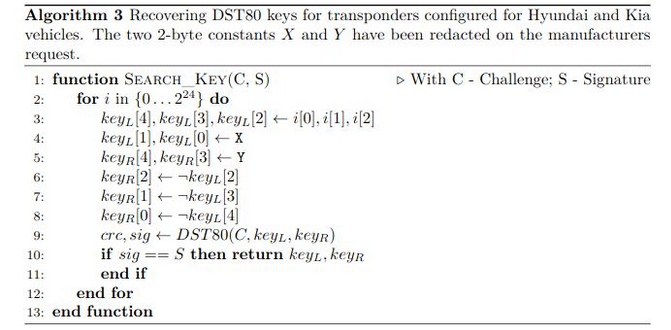
\includegraphics[keepaspectratio]{pictures/iacr.png}}
\caption{IACR Algorithm}
\end{figure}

\subsubsection{Constantes inconnues}\label{constantes-inconnues}

Sur un GPU grand public (par exemple \textbf{NVIDIA RTX 3050 Ti}),
récupérer une clé complète avec \textbf{un octet inconnu} prend environ
:

\textbf{300 minutes (\textasciitilde5 heures)}.

\subsubsection{Constantes connues}\label{constantes-connues}

Une fois les constantes constructeur identifiées, l'espace de recherche
se réduit drastiquement :

\textbf{environ 1 minute} pour retrouver une clé.

\subsubsection{Changement de
constructeur}\label{changement-de-constructeur}

Si le constructeur change, il suffit de :

\begin{enumerate}
\def\labelenumi{\arabic{enumi}.}
\tightlist
\item
  retrouver les nouvelles constantes
\item
  puis revenir au temps de récupération d'environ \textbf{1 minute par
  clé}.
\end{enumerate}

\begin{center}\rule{0.5\linewidth}{0.5pt}\end{center}

\subsection{Configuration
matérielle}\label{configuration-matuxe9rielle-1}

\begin{itemize}
\item
  \textbf{GPU} : tout GPU compatible \textbf{OpenCL}

  \begin{itemize}
  \tightlist
  \item
    NVIDIA
  \item
    AMD
  \item
    Intel
  \end{itemize}
\item
  \textbf{Testé sur} :

  \begin{itemize}
  \tightlist
  \item
    NVIDIA GeForce \textbf{RTX 3050 Ti Laptop GPU}
  \end{itemize}
\item
  \textbf{Performance observée} :
\end{itemize}

\begin{verbatim}
~35 millions de clés testées par seconde
\end{verbatim}

\begin{center}\rule{0.5\linewidth}{0.5pt}\end{center}

\subsection{Structure du projet}\label{structure-du-projet}

\begin{longtable}[]{@{}
  >{\raggedright\arraybackslash}p{(\linewidth - 2\tabcolsep) * \real{0.1930}}
  >{\raggedright\arraybackslash}p{(\linewidth - 2\tabcolsep) * \real{0.8070}}@{}}
\toprule\noalign{}
\begin{minipage}[b]{\linewidth}\raggedright
Fichier
\end{minipage} & \begin{minipage}[b]{\linewidth}\raggedright
Description
\end{minipage} \\
\midrule\noalign{}
\endhead
\bottomrule\noalign{}
\endlastfoot
\texttt{dst80\_fast.py} & Recherche optimisée utilisant un octet
constructeur fixe (\texttt{0x2f}). \\
\texttt{dst80\_constructor.py} & Permet de passer deux octets
constructeur (\texttt{m2}, \texttt{m1}) en argument. \\
\texttt{dst80\_reverse.py} & Recherche complète (jusqu'à 5 octets) pour
identifier les constantes constructeur inconnues. \\
\texttt{*.cl} & Kernels OpenCL contenant la simulation du chiffrement
DST80. \\
\end{longtable}

\begin{center}\rule{0.5\linewidth}{0.5pt}\end{center}

\subsection{Utilisation}\label{utilisation}

\subsubsection{Installation}\label{installation}

\begin{Shaded}
\begin{Highlighting}[]
\ExtensionTok{pip}\NormalTok{ install }\AttributeTok{{-}r}\NormalTok{ requirements.txt}
\end{Highlighting}
\end{Shaded}

\begin{center}\rule{0.5\linewidth}{0.5pt}\end{center}

\subsubsection{Recherche rapide (constante 1 octet
connue)}\label{recherche-rapide-constante-1-octet-connue}

Si vous connaissez le suffixe (par exemple \texttt{0x2f}) :

\begin{Shaded}
\begin{Highlighting}[]
\ExtensionTok{python}\NormalTok{ dst80\_fast.py }\OperatorTok{\textless{}}\NormalTok{c1}\OperatorTok{\textgreater{}} \OperatorTok{\textless{}}\NormalTok{t1}\OperatorTok{\textgreater{}} \OperatorTok{\textless{}}\NormalTok{c2}\OperatorTok{\textgreater{}} \OperatorTok{\textless{}}\NormalTok{t2}\OperatorTok{\textgreater{}}
\end{Highlighting}
\end{Shaded}

\begin{center}\rule{0.5\linewidth}{0.5pt}\end{center}

\subsubsection{Recherche constructeur (constantes 2
octets)}\label{recherche-constructeur-constantes-2-octets}

Pour tester des constantes constructeur spécifiques (exemple
\texttt{d1\ 2f}) :

\begin{Shaded}
\begin{Highlighting}[]
\ExtensionTok{python}\NormalTok{ dst80\_constructor.py }\OperatorTok{\textless{}}\NormalTok{c1}\OperatorTok{\textgreater{}} \OperatorTok{\textless{}}\NormalTok{t1}\OperatorTok{\textgreater{}} \OperatorTok{\textless{}}\NormalTok{c2}\OperatorTok{\textgreater{}} \OperatorTok{\textless{}}\NormalTok{t2}\OperatorTok{\textgreater{}}\NormalTok{ d1 2f}
\end{Highlighting}
\end{Shaded}

\begin{center}\rule{0.5\linewidth}{0.5pt}\end{center}

\subsubsection{Reverse complet (mode
découverte)}\label{reverse-complet-mode-duxe9couverte}

Pour explorer l'espace complet (5 octets variables) afin de trouver les
constantes :

\begin{Shaded}
\begin{Highlighting}[]
\ExtensionTok{python}\NormalTok{ dst80\_reverse.py }\OperatorTok{\textless{}}\NormalTok{c1}\OperatorTok{\textgreater{}} \OperatorTok{\textless{}}\NormalTok{t1}\OperatorTok{\textgreater{}} \OperatorTok{\textless{}}\NormalTok{c2}\OperatorTok{\textgreater{}} \OperatorTok{\textless{}}\NormalTok{t2}\OperatorTok{\textgreater{}}\NormalTok{ 4228250625}
\end{Highlighting}
\end{Shaded}

\begin{center}\rule{0.5\linewidth}{0.5pt}\end{center}

\subsection{Démonstration}\label{duxe9monstration}

Ci-dessous un exemple de récupération réussie d'une clé avec la méthode
\textbf{double challenge}.

\begin{figure}
\centering
\pandocbounded{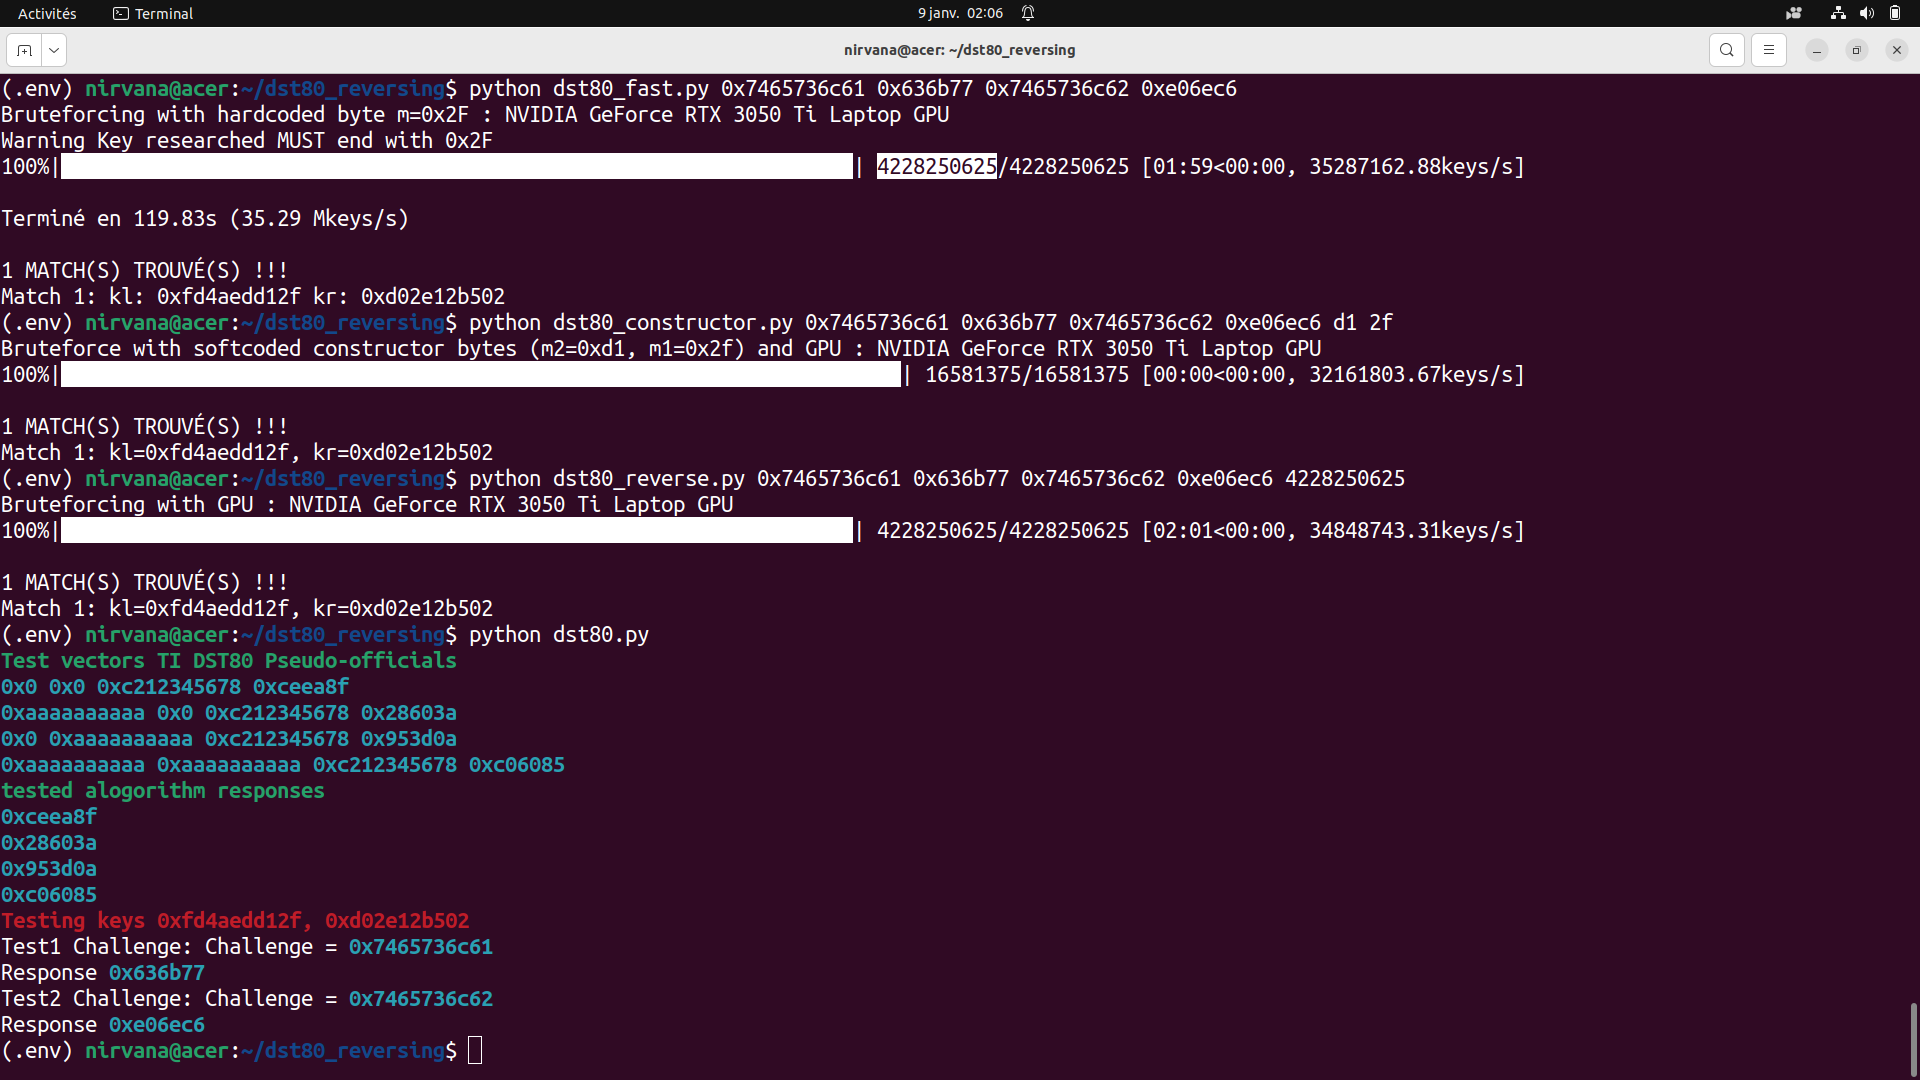
\includegraphics[keepaspectratio]{pictures/demo.png}}
\caption{Search Demo}
\end{figure}

\begin{center}\rule{0.5\linewidth}{0.5pt}\end{center}

\subsection{Tutoriel : générateur de signature
DST80}\label{tutoriel-guxe9nuxe9rateur-de-signature-dst80}

Ce script calcule la \textbf{réponse de 24 bits (signature)} pour un
challenge DST80 donné.

Il gère automatiquement la \textbf{symétrie interne du chiffrement} en
dérivant \textbf{Key Right (KR)} à partir de \textbf{Key Left (KL)}.

\begin{center}\rule{0.5\linewidth}{0.5pt}\end{center}

\subsection{Construction de la clé}\label{construction-de-la-cluxe9}

Le script suppose l'implémentation automobile classique où la clé de
\textbf{80 bits est symétrique} :

\begin{itemize}
\item
  \textbf{KeyL (40 bits)} fourni par l'utilisateur.
\item
  \textbf{KeyR (40 bits)} généré automatiquement en \textbf{inversant
  chaque octet de KeyL}.
\end{itemize}

\begin{center}\rule{0.5\linewidth}{0.5pt}\end{center}

\subsection{Utilisation basique}\label{utilisation-basique}

Lancer simplement le script pour utiliser les valeurs par défaut :

\begin{Shaded}
\begin{Highlighting}[]
\ExtensionTok{python}\NormalTok{ generate.py}
\end{Highlighting}
\end{Shaded}

Cela permet de \textbf{vérifier que l'environnement fonctionne
correctement}.

\begin{center}\rule{0.5\linewidth}{0.5pt}\end{center}

\subsection{Challenges et clés
personnalisés}\label{challenges-et-cluxe9s-personnalisuxe9s}

Vous pouvez fournir vos propres valeurs hexadécimales.

\subsubsection{Signer un challenge
spécifique}\label{signer-un-challenge-spuxe9cifique}

\begin{Shaded}
\begin{Highlighting}[]
\ExtensionTok{python}\NormalTok{ generate.py }\AttributeTok{{-}{-}challenge}\NormalTok{ 0xABCDE12345}
\end{Highlighting}
\end{Shaded}

\begin{center}\rule{0.5\linewidth}{0.5pt}\end{center}

\subsubsection{Utiliser une clé
récupérée}\label{utiliser-une-cluxe9-ruxe9cupuxe9ruxe9e}

\begin{Shaded}
\begin{Highlighting}[]
\ExtensionTok{python}\NormalTok{ generate.py }\AttributeTok{{-}{-}kl}\NormalTok{ 0xFD4AEDD12F}
\end{Highlighting}
\end{Shaded}

\begin{center}\rule{0.5\linewidth}{0.5pt}\end{center}

\subsubsection{Commande complète}\label{commande-compluxe8te}

\begin{Shaded}
\begin{Highlighting}[]
\ExtensionTok{python}\NormalTok{ generate.py }\AttributeTok{{-}{-}kl}\NormalTok{ 0x1122334455 }\AttributeTok{{-}{-}challenge}\NormalTok{ 0x6162636465}
\end{Highlighting}
\end{Shaded}

\begin{center}\rule{0.5\linewidth}{0.5pt}\end{center}

\subsection{Détail de la sortie}\label{duxe9tail-de-la-sortie}

Le script affiche un résumé clair :

\begin{itemize}
\tightlist
\item
  \textbf{KeyL} : clé source (40 bits)
\item
  \textbf{KeyR} : clé miroir générée
\item
  \textbf{Challenge} : nonce d'entrée (40 bits)
\item
  \textbf{RESPONSE} : signature finale \textbf{0xXXXXXX} utilisée pour
  l'authentification
\end{itemize}

\section{Le réseau TETRA}\label{le-ruxe9seau-tetra}

Le \textbf{TETRA (Terrestrial Trunked Radio)} est une norme de
communication radio numérique conçue pour les \textbf{services
critiques}. Elle a été développée dans les années 1990 par
l'\textbf{European Telecommunications Standards Institute} pour
remplacer les anciens réseaux radio analogiques utilisés par les
services publics.

Contrairement aux réseaux cellulaires grand public, TETRA est destiné à
des organisations qui ont besoin de communications \textbf{fiables,
sécurisées et instantanées}, même dans des situations de crise.

On le retrouve notamment dans :

\begin{itemize}
\tightlist
\item
  les \textbf{polices}
\item
  les \textbf{services de secours}
\item
  les \textbf{pompiers}
\item
  les \textbf{services de transport}
\item
  les \textbf{infrastructures critiques}
\end{itemize}

Dans plusieurs pays européens, les réseaux TETRA sont utilisés par les
services d'urgence nationaux.

\begin{center}\rule{0.5\linewidth}{0.5pt}\end{center}

\subsection{Principe général}\label{principe-guxe9nuxe9ral}

Un réseau TETRA est un \textbf{réseau radio professionnel trunké}. Le
terme \emph{trunked radio} signifie que les utilisateurs partagent
dynamiquement un ensemble de canaux radio.

Au lieu d'avoir une fréquence fixe pour chaque groupe, le système
attribue automatiquement les canaux disponibles.

Architecture simplifiée :

\begin{verbatim}
terminaux radio
      ↓
stations de base (TBS)
      ↓
commutation réseau
      ↓
groupes utilisateurs
\end{verbatim}

Les terminaux sont généralement des \textbf{talkies-walkies numériques}
capables de fonctionner :

\begin{itemize}
\tightlist
\item
  en \textbf{mode réseau}
\item
  en \textbf{mode direct (DMO)} sans infrastructure
\end{itemize}

\begin{center}\rule{0.5\linewidth}{0.5pt}\end{center}

\subsection{Architecture du réseau}\label{architecture-du-ruxe9seau}

Un réseau TETRA comporte plusieurs éléments principaux.

\subsubsection{Terminaux radio}\label{terminaux-radio}

Les terminaux sont des radios portables ou embarquées dans des
véhicules. Ils permettent plusieurs types de communication :

\begin{itemize}
\tightlist
\item
  appels individuels
\item
  appels de groupe
\item
  messages de données
\item
  signalisation d'urgence
\end{itemize}

La communication de groupe est l'une des fonctions centrales du système.

\begin{center}\rule{0.5\linewidth}{0.5pt}\end{center}

\subsubsection{Stations de base}\label{stations-de-base}

Les stations de base assurent la couverture radio d'une zone.

Chaque station gère plusieurs canaux radio et communique avec le réseau
central.

Ces stations sont appelées :

\textbf{TBS --- TETRA Base Station}

\begin{center}\rule{0.5\linewidth}{0.5pt}\end{center}

\subsubsection{Commutation réseau}\label{commutation-ruxe9seau}

Le cœur du réseau TETRA est un système de commutation qui gère :

\begin{itemize}
\tightlist
\item
  l'attribution des canaux
\item
  les groupes d'utilisateurs
\item
  la mobilité
\item
  l'authentification
\end{itemize}

Ce composant est appelé :

\textbf{SwMI --- Switching and Management Infrastructure}

Il joue un rôle comparable au \textbf{MSC} dans les réseaux GSM.

\begin{center}\rule{0.5\linewidth}{0.5pt}\end{center}

\subsection{Caractéristiques radio}\label{caractuxe9ristiques-radio}

TETRA utilise une bande radio dédiée, généralement autour de :

\begin{verbatim}
380 – 400 MHz
\end{verbatim}

(services de sécurité publique en Europe)

La technologie utilise :

\begin{verbatim}
TDMA
Time Division Multiple Access
\end{verbatim}

Chaque canal radio de \textbf{25 kHz} est divisé en \textbf{4 slots
temporels}.

\begin{verbatim}
| slot1 | slot2 | slot3 | slot4 |
\end{verbatim}

Cela permet à plusieurs utilisateurs de partager la même fréquence.

Le débit typique est d'environ :

\begin{verbatim}
7.2 kb/s par slot
\end{verbatim}

\begin{center}\rule{0.5\linewidth}{0.5pt}\end{center}

\subsection{Fonctionnalités
principales}\label{fonctionnalituxe9s-principales}

Le système TETRA est conçu pour répondre aux besoins des communications
critiques.

\subsubsection{Appel de groupe}\label{appel-de-groupe}

Un utilisateur peut parler simultanément à tout un groupe
d'utilisateurs.

Exemple :

\begin{verbatim}
pompiers secteur A
\end{verbatim}

Un seul bouton permet de transmettre à l'ensemble du groupe.

\begin{center}\rule{0.5\linewidth}{0.5pt}\end{center}

\subsubsection{Communication
instantanée}\label{communication-instantanuxe9e}

Contrairement à un appel téléphonique, la communication est quasi
instantanée.

Le temps d'établissement est typiquement :

\begin{verbatim}
< 300 ms
\end{verbatim}

\begin{center}\rule{0.5\linewidth}{0.5pt}\end{center}

\subsubsection{Mode direct (DMO)}\label{mode-direct-dmo}

Les terminaux peuvent communiquer directement entre eux sans station de
base.

\begin{verbatim}
radio ↔ radio
\end{verbatim}

Ce mode est utile lorsque l'infrastructure est indisponible.

\begin{center}\rule{0.5\linewidth}{0.5pt}\end{center}

\subsubsection{Priorité et appels
d'urgence}\label{priorituxe9-et-appels-durgence}

Certains utilisateurs peuvent avoir un niveau de priorité supérieur.

Par exemple :

\begin{itemize}
\tightlist
\item
  chef d'intervention
\item
  centre de commandement
\end{itemize}

Un appel prioritaire peut interrompre les communications en cours.

\begin{center}\rule{0.5\linewidth}{0.5pt}\end{center}

\subsection{Sécurité}\label{suxe9curituxe9}

Les réseaux TETRA intègrent plusieurs mécanismes de sécurité :

\begin{itemize}
\tightlist
\item
  \textbf{authentification des terminaux}
\item
  \textbf{chiffrement des communications}
\item
  \textbf{gestion des clés}
\end{itemize}

Le chiffrement est généralement basé sur des algorithmes propriétaires
appelés :

\begin{verbatim}
TEA — TETRA Encryption Algorithm
\end{verbatim}

Il existe plusieurs variantes :

\begin{itemize}
\tightlist
\item
  TEA1
\item
  TEA2
\item
  TEA3
\item
  TEA4
\end{itemize}

Certaines implémentations ont fait l'objet de recherches de sécurité
récentes montrant des faiblesses dans certaines variantes.

\begin{center}\rule{0.5\linewidth}{0.5pt}\end{center}

\subsection{Utilisations}\label{utilisations}

Les réseaux TETRA sont largement utilisés dans le monde pour les
communications professionnelles.

Exemples d'applications :

\begin{itemize}
\tightlist
\item
  réseaux de police
\item
  services d'urgence
\item
  contrôle ferroviaire
\item
  gestion d'aéroports
\item
  transports publics
\end{itemize}

Ils offrent un avantage important : ils restent \textbf{opérationnels
même en cas de surcharge des réseaux mobiles classiques}.

\begin{center}\rule{0.5\linewidth}{0.5pt}\end{center}

\subsection{Limites}\label{limites}

Bien que très robuste, la technologie TETRA présente certaines limites :

\begin{itemize}
\tightlist
\item
  faible débit de données
\item
  technologie principalement conçue pour la voix
\item
  coût d'infrastructure élevé
\end{itemize}

Pour ces raisons, certains réseaux critiques migrent progressivement
vers des solutions basées sur \textbf{LTE ou 5G mission-critical}.

Cependant, TETRA reste aujourd'hui l'une des infrastructures radio les
plus fiables pour les communications de sécurité publique.

\subsubsection{Chiffrement TETRA et vulnérabilités révélées par Midnight
Blue
(2023)}\label{chiffrement-tetra-et-vulnuxe9rabilituxe9s-ruxe9vuxe9luxe9es-par-midnight-blue-2023}

Les réseaux \textbf{TETRA (Terrestrial Trunked Radio)} utilisent un
mécanisme de chiffrement spécifique appelé \textbf{TEA --- TETRA
Encryption Algorithm}. Ces algorithmes sont conçus pour protéger les
communications des réseaux professionnels utilisés par les services
critiques.

Les différentes variantes de l'algorithme sont :

\begin{itemize}
\tightlist
\item
  \textbf{TEA1}
\item
  \textbf{TEA2}
\item
  \textbf{TEA3}
\item
  \textbf{TEA4}
\end{itemize}

Chaque variante correspond à un niveau d'utilisation différent :

\begin{longtable}[]{@{}ll@{}}
\toprule\noalign{}
Algorithme & Utilisation \\
\midrule\noalign{}
\endhead
\bottomrule\noalign{}
\endlastfoot
TEA1 & réseaux commerciaux et infrastructures civiles \\
TEA2 & réseaux de sécurité publique (police, armée) \\
TEA3 & export hors Europe \\
TEA4 & usage industriel \\
\end{longtable}

Pendant longtemps, les spécifications détaillées de ces algorithmes sont
restées \textbf{confidentielles} et uniquement accessibles aux
fabricants agréés.

\begin{center}\rule{0.5\linewidth}{0.5pt}\end{center}

\subsection{La révélation de 2023}\label{la-ruxe9vuxe9lation-de-2023}

En \textbf{2023}, une équipe de chercheurs en sécurité de la société
\textbf{Midnight Blue} publie une analyse détaillée du système de
sécurité TETRA.

Cette recherche révèle une série de vulnérabilités regroupées sous le
nom :

\begin{verbatim}
TETRA:BURST
\end{verbatim}

Ces vulnérabilités ont été enregistrées sous plusieurs identifiants
\textbf{CVE-2023}.

Les chercheurs ont montré que certaines implémentations du chiffrement
TETRA présentaient des faiblesses significatives, notamment dans
\textbf{TEA1}.

\begin{center}\rule{0.5\linewidth}{0.5pt}\end{center}

\subsection{Faiblesse principale de
TEA1}\label{faiblesse-principale-de-tea1}

L'une des découvertes majeures concerne la taille réelle de la clé.

Bien que TEA1 soit présenté comme utilisant une clé de \textbf{80 bits},
l'analyse a montré que la conception du système réduit en pratique
l'espace de recherche à environ :

\begin{verbatim}
2^32
\end{verbatim}

Autrement dit, le chiffrement peut être attaqué avec un \textbf{brute
force réalisable sur du matériel moderne}.

Avec un GPU moderne, une recherche exhaustive peut être réalisée en
quelques minutes ou heures.

Cette faiblesse provient notamment :

\begin{itemize}
\tightlist
\item
  d'une réduction effective de l'entropie
\item
  d'un design interne affaiblissant la sécurité
\item
  de choix cryptographiques hérités des années 1990
\end{itemize}

\begin{center}\rule{0.5\linewidth}{0.5pt}\end{center}

\subsection{Vulnérabilités
identifiées}\label{vulnuxe9rabilituxe9s-identifiuxe9es}

Les chercheurs ont identifié plusieurs problèmes dans l'écosystème TETRA
:

\subsubsection{Réduction de la taille de
clé}\label{ruxe9duction-de-la-taille-de-cluxe9}

Le chiffrement TEA1 présente une \textbf{clé effective fortement
réduite}, permettant une attaque brute force.

\begin{center}\rule{0.5\linewidth}{0.5pt}\end{center}

\subsubsection{Faiblesse dans
l'authentification}\label{faiblesse-dans-lauthentification}

Certaines implémentations permettent des attaques permettant de :

\begin{itemize}
\tightlist
\item
  intercepter des communications
\item
  injecter des paquets radio
\item
  perturber le réseau
\end{itemize}

\begin{center}\rule{0.5\linewidth}{0.5pt}\end{center}

\subsubsection{Problèmes de gestion de
clés}\label{probluxe8mes-de-gestion-de-cluxe9s}

Certaines infrastructures TETRA utilisent des mécanismes de distribution
de clés vulnérables.

\begin{center}\rule{0.5\linewidth}{0.5pt}\end{center}

\subsection{Impact potentiel}\label{impact-potentiel}

Les réseaux TETRA sont utilisés dans de nombreux systèmes critiques :

\begin{itemize}
\tightlist
\item
  police
\item
  pompiers
\item
  transports publics
\item
  infrastructures énergétiques
\item
  services d'urgence
\end{itemize}

La découverte de ces vulnérabilités a donc un impact potentiel
important.

Cependant, plusieurs facteurs limitent les risques immédiats :

\begin{itemize}
\tightlist
\item
  certaines variantes comme \textbf{TEA2} ne sont pas concernées par la
  même faiblesse
\item
  les réseaux utilisent souvent des mécanismes supplémentaires de
  sécurité
\item
  l'exploitation nécessite des équipements radio spécialisés
\end{itemize}

\begin{center}\rule{0.5\linewidth}{0.5pt}\end{center}

\subsection{Importance pour la recherche en sécurité
radio}\label{importance-pour-la-recherche-en-suxe9curituxe9-radio}

L'étude publiée par Midnight Blue marque un tournant dans l'analyse des
réseaux radio professionnels.

Pendant longtemps, les protocoles TETRA étaient considérés comme
\textbf{opaques et difficilement analysables}.

Grâce aux progrès des \textbf{Software Defined Radios (SDR)} et aux
recherches en sécurité radio, il devient désormais possible de :

\begin{itemize}
\tightlist
\item
  analyser les signaux TETRA
\item
  étudier les protocoles de chiffrement
\item
  tester la robustesse des systèmes radio critiques
\end{itemize}

Ces travaux illustrent un principe fondamental de la sécurité
informatique :

\begin{quote}
la sécurité par le secret du design est rarement durable.
\end{quote}

Les systèmes cryptographiques doivent être \textbf{ouverts à l'analyse
publique} afin de garantir leur robustesse.

\subsection{TEA1 Key Brute-forcer (OpenCL
Accelerated)}\label{tea1-key-brute-forcer-opencl-accelerated}

\href{https://github.com/bbaranoff/tea1-cracker}{tea1 cracker} Ce projet
est un outil de recherche de clé pour l'algorithme de chiffrement
\textbf{TEA1}. Il utilise la puissance de calcul parallèle des
processeurs graphiques (\textbf{GPU}) via \textbf{OpenCL} pour tester
l'intégralité de l'espace des clés (32 bits) en un temps record.

\subsubsection{Principe de
fonctionnement}\label{principe-de-fonctionnement-1}

Le script repose sur une attaque par \textbf{force brute à texte clair
connu (Known Plaintext Attack)}. Si vous disposez d'un fragment du flux
chiffré et que vous connaissez (ou devinez) le contenu original, vous
pouvez isoler le \textbf{Keystream}.

\subsubsection{Inversion du Keystream}\label{inversion-du-keystream}

TEA1 est un chiffrement de flux. Le processus est le suivant :

Le script prend en entrée 64 bits (16 caractères hexadécimaux) de ce
keystream pour valider si une clé candidate est la bonne.

\subsubsection{Algorithme de recherche}\label{algorithme-de-recherche}

\begin{itemize}
\tightlist
\item
  \textbf{Initialisation de l'IV} : Le script reconstruit l'Instruction
  Vector (IV) à partir des paramètres de trame (Timeslot, Frame Number,
  etc.) via la fonction \texttt{build\_iv}.
\item
  \textbf{Parallélisation GPU} : L'espace de recherche de clés est
  divisé en paquets (batches). Le kernel OpenCL teste simultanément des
  milliers de clés.
\item
  \textbf{Validation 64-bit} : Contrairement aux versions simplifiées
  qui testent 32 bits, ce script vérifie 64 bits du keystream pour
  éliminer les ``fausses alertes'' (collisions) et garantir que la clé
  trouvée est l'unique clé correcte.
\end{itemize}

\begin{center}\rule{0.5\linewidth}{0.5pt}\end{center}

\subsection{Utilisation}\label{utilisation-1}

\subsubsection{Prérequis}\label{pruxe9requis-3}

\begin{itemize}
\tightlist
\item
  Un GPU compatible OpenCL.
\item
  Python 3.x avec les bibliothèques : \texttt{pyopencl}, \texttt{numpy}.
\end{itemize}

\subsubsection{Syntaxe}\label{syntaxe}

Le script requiert les paramètres réseau de la trame interceptée pour
synchroniser l'état interne de l'algorithme.

\begin{Shaded}
\begin{Highlighting}[]
\ExtensionTok{python}\NormalTok{ crack\_tea1.py }\OperatorTok{\textless{}}\NormalTok{TN}\OperatorTok{\textgreater{}} \OperatorTok{\textless{}}\NormalTok{HN}\OperatorTok{\textgreater{}} \OperatorTok{\textless{}}\NormalTok{MN}\OperatorTok{\textgreater{}} \OperatorTok{\textless{}}\NormalTok{FN}\OperatorTok{\textgreater{}} \OperatorTok{\textless{}}\NormalTok{SN}\OperatorTok{\textgreater{}} \OperatorTok{\textless{}}\NormalTok{Direction}\OperatorTok{\textgreater{}} \OperatorTok{\textless{}}\NormalTok{Keystream\_Hex}\OperatorTok{\textgreater{}}
\end{Highlighting}
\end{Shaded}

\textbf{Arguments :}

\begin{itemize}
\tightlist
\item
  \texttt{TN}, \texttt{HN}, \texttt{MN}, \texttt{FN} : Numéros de trames
  et slots (Time/Hyper/Macro/Frame numbers).
\item
  \texttt{Direction} : 0 ou 1 (Uplink/Downlink).
\item
  \texttt{Keystream\_Hex} : Les 16 premiers caractères hexadécimaux du
  keystream extrait.
\end{itemize}

\textbf{Exemple :}

\begin{Shaded}
\begin{Highlighting}[]
\ExtensionTok{python}\NormalTok{ tea1\_opencl\_crack.py 1 110 30 06 1 0 0BE7FE9AE1EA459F866919C9E2EA1E11A77A4493D658A4191EDD987F37DE12B1DA3F7BBD62607E8CE787C2FE544B2FAAEAED38255BEB}
\end{Highlighting}
\end{Shaded}

\begin{center}\rule{0.5\linewidth}{0.5pt}\end{center}

\subsection{Performance et Impact}\label{performance-et-impact}

\subsubsection{Impact Technique}\label{impact-technique}

\begin{itemize}
\tightlist
\item
  \textbf{Vitesse} : Sur un GPU de milieu de gamme, l'intégralité de
  l'espace de clé 32 bits peut être parcourue en quelques minutes (voire
  secondes), contre plusieurs heures sur un CPU classique.
\item
  \textbf{Sécurité} : Cet outil démontre la faiblesse critique de TEA1.
  Avec une clé de seulement 32 bits d'entropie effective, le chiffrement
  ne résiste pas à une analyse computationnelle moderne.
\end{itemize}

\subsubsection{Limites}\label{limites-1}

\begin{itemize}
\tightlist
\item
  \textbf{Accès au Keystream} : L'utilisateur doit être capable
  d'identifier au moins 8 octets de données connues (comme des en-têtes
  LLC ou IP) pour extraire le keystream.
\item
  \textbf{Matériel} : La performance dépend directement du nombre
  d'unités de calcul (Compute Units) du GPU utilisé.
\end{itemize}

\end{document}
